%\epigraphfontsize{\small\itshape}
%\setlength\epigraphwidth{8cm}
%\setlength\epigraphrule{0pt}
%\epigraphfontsize{\small\itshape}

%\epigraph{There are two possible outcomes: If the result confirms the hypothesis, then you've made a measurement. If the result is contrary to the hypothesis, then you've made a discovery.}{---\textup{ Enrico Fermi}}
%\epigraph{Everyone knows how useful it is to be useful. No one seems to know how useful it is to be useless.}{---\textup{  Chuang Tzu, The Useless Tree}}
\section{An Overview of the Reconstruction Algorithms in SNO+}
A particle interaction that happens in the SNO+ detector can produce Cherenkov or scintillation photons. These photons propagate through the detector, and they can trigger PMTs when they reach the PSUP. As described in the last chapter, if there are enough PMTs triggered within a defined time window, an event is determined by the trigger system, and for the event, the time and charge information measured by the hit PMTs are recorded.

By utilizing the recorded time and charge information, reconstruction algorithms attempt to calculate the physics quantities of an event, including its vertex (position and time), direction, and energy. A few sets of reconstruction algorithms (called ``fitters'') have been implemented in the SNO+ RAT software or are still being developed. These fitters are based on different methods and can be coordinated and optimized for the different detector situations or physics phases.

According to the physics quantities, the SNO+ fitters can be generally classified as:
\begin{itemize}
	\item Vertex fitter. A vertex fitter reconstructs the event position and time by utilizing the positions and timing information of the hit PMTs. Currently, vertex fitters have been used to process the data and simulations for the water and partial-fill phases. They are also ready for the scintillator and tellurium-loading phases.
	
    On the other hand, some particular events, such as radioactive background events emitting $\gamma$s, can create multiple correlated vertices. A multi-site or multi-vertex fitter will be helpful in tagging and removing these events during the $0\nu\beta\beta$ search. This kind of fitter is being developed.

	\item Direction fitter. A direction fitter reconstructs the event direction by using the directional information from the Cherenkov photons, which cause ring-like patterns formed by the hit PMT positions. The direction fitter has been used in the water phase analysis. For the scintillator and tellurium-loading phases, since the Cherenkov patterns will be submerged in the scintillation photons, it requires other efforts for the direction reconstruction, which is being developed currently. 
	
	\item Energy fitter. An energy fitter translates the number of photons created from an event to kinetic energy. Similar to the vertex fitters, the energy fitters currently have been used in the water and partial-fill phases, and they are ready for the scintillator and tellurium-loading phases.

	\item Muon track fitter. This fitter is used to reconstruct the tracks of cosmic muons. It treats a muon track as a straight line, and by dividing the SNO+ detector into several XY-slices along z, it reconstructs the intersection points for each slice by utilizing the positions and timing information of the hit PMTs\cite{muonTrackRecon}. It is currently being developed for the scintillator and tellurium-loading phases. It will help to tag and reduce the cosmogenic backgrounds, especially the $^{11}$C backgrounds induced by the muon spallation on the liquid scintillators\cite{sorensen2016temperature}.
\end{itemize}

For a fitter, its performance is first tested on the Monte Carlo simulations of specific physics processes. Then it is tested on both the simulations and data of the calibration runs. Once the algorithm gives good results and is approved by the SNO+ collaboration, it is implemented into the SNO+ RAT software to process the SNO+ simulations and data files.

For a specific SNO+ physics phase, the fitters for reconstructing different physics quantities of an event are integrated. Currently, there are three integrated fitters: the \texttt{Water Fitter} for the water phase, the \texttt{Partial Fitter} for the partial-fill phase, and the \texttt{Scint Fitter} for the scintillator phase and the tellurium loading phase. The fitter parameters, such as the optical parameters, fitter iterations, are coordinated and optimized based on simulations and calibration data from that specific physics phase. In addition, PMT selectors and classifiers are also included in the integrated fitters. The PMT selectors are used to remove the outliers of the hit PMTs for a specific fitter, such as the hit PMT probably triggered by the noises. These selectors can help to make the fitter more accurate or to boost up the fitter speed. The classifiers mainly use the reconstructed results to calculate specific quantities which describe the probability of determining an event as an expected signal or background.

In this chapter, a Multi-path (MP) reconstruction framework and its principles are discussed. It was developed by the University of Alberta group as an additional fitter to provide event vertex and direction reconstructions. In this framework, the fitters can be adapted for all the SNO+ physics phases by switching light path calculations, input parameters such as the optical parameters and the detector state. That is the reason why it is called "multiple paths".  It was applied in the water phase to provide alternative information of the event position and direction; it also works as the vertex reconstruction algorithm for the \texttt{Partial Fitter}. After re-coordination for the scintillator and tellurium loading phases, I also show the potentials of the vertex fitter being applied in these two future phases.

In addition, the potentials of extracting the directional information from the scintillator phase are also discussed in this chapter.

\section{Multi-path Position and Direction Reconstructions for the Water Phase}\label{sect:mpw}
In the SNO+ water phase, both the cavity and the AV were filled with ultra-pure water. In this case, the detector geometry is simple since everything inside the PSUP sphere can be simplified as water if omitting the AV shell. Therefore, to explain the reconstruction concepts, I will start with the \texttt{MP water fitter} (the \texttt{MPW fitter}).

The \texttt{MPW fitter} fits for the vertex and direction of a triggered event in the SNO+ water phase. It first fits for the event vertex and then takes the results of the reconstructed position to fit for the event direction.

\subsection{Vertex Reconstruction}\label{sect:waterVertex}

To fit for the vertex with four parameters: $x,y,z$ and $t$, first the fitter creates a random position inside a sphere with a radius of $10~m$ (larger than the actual PSUP radius $r_{PSUP}=8.39~m$). Meanwhile, a random event time is also generated from a uniform distribution in the range of $[100,300~ns]$. The Class Library for High Energy Physics (\texttt{CLHEP}) is used for creating pseudo-random numbers. The random position and the random time are combined to form a random event vertex as the trial event vertex $\vec{X}_0$. See the Sect.~\ref{appendix:random_gen} for details.

For a triggered event, photons are created around the event position and propagate to the hit PMTs. In a simplified detector geometry model that neglects the effects of scattering, reflection, and refraction, these photons are considered as propagating along straight lines connecting the trial event vertex to the hit PMTs. Then the fitter evaluates a timing parameter, called the time residual ($t_{res}$), which is defined as:
\begin{equation}
\label{eq:tres_define}
t_{res}=t_\mathrm{PMT} - t_{transit} - t_{event},
\end{equation}
where $t_\mathrm{PMT}$ is the PMT trigger time recorded by the detector, $t_{event}$ is the time when an event occurs (event time), and $t_{transit}$ is the total transit time (or time of flight, $TOF$) taken by a photon traveling from the event position ($\vec{X}_{event}$) to the hit PMT ($\vec{X}_{PMT}$) and crossing different materials in the detector.

To calculate the $t_{transit}$, the fitter uses Cherenkov photons in a prompt time window (called ``prompt light''), set as $-10<t_{res}<10~ns$ for the \texttt{MPW fitter} and the photons are assumed to propagate in straight lines (straight light paths). By assuming straight light paths, complicated situations of the photon propagation are neglected, including the refraction and reflection when the lights cross boundaries between different detector materials, absorption and scattering from the materials, and the lensing effects caused by the spherical structure of the acrylic vessel. In this case, the $TOF$ can be simply calculated as $t_{transit}=|\vec{X}_{event}-\vec{X}_{PMT}|/v_{water}$, where $v_{water}$ is an average photon group velocity and it is an effective value obtained by tuning on the Monte Carlo simulations. Section \ref{sect:tuneGroupVelocity} will show the details about the tuning. Based on the reconstruction experiences from the SNO experiment, it found that without these details, the fitter can still produce decent results that are consistent with the case using detailed calculations\cite{boulay2004direct,jones2011background}. Fig.~\ref{mpwdiagram_position} shows the straight light paths from the event position to the hit PMT positions.
\begin{figure}[htbp]
	\centering
   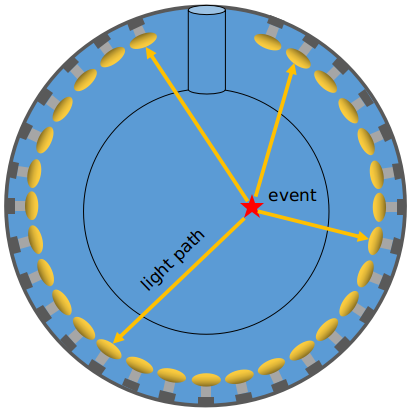
\includegraphics[width=6cm]{mpwDiagram.png}
	\caption[Straight light path calculation in the water geometry.]{A diagram of straight light path for event position reconstruction in the SNO+ water phase geometry.}
	\label{mpwdiagram_position}
\end{figure}

An one-dimensional (1D) probability density function ($PDF$) is used for fitting the timing model, as shown in Fig.~\ref{fig:MPW_timingPDF}. This $PDF$ serves as a model of the timing responses of the triggered PMTs to an event to be fit. It was taken from the bench-top measurement of the individual PMT time profile from SNO\cite{jillings1996photomultiplier} and was further tuned according to the measured \emph{in-situ} SNO+ detector responses to the calibration sources\cite{anderson2021optical}.

\begin{figure}[!htb]
	\centering
	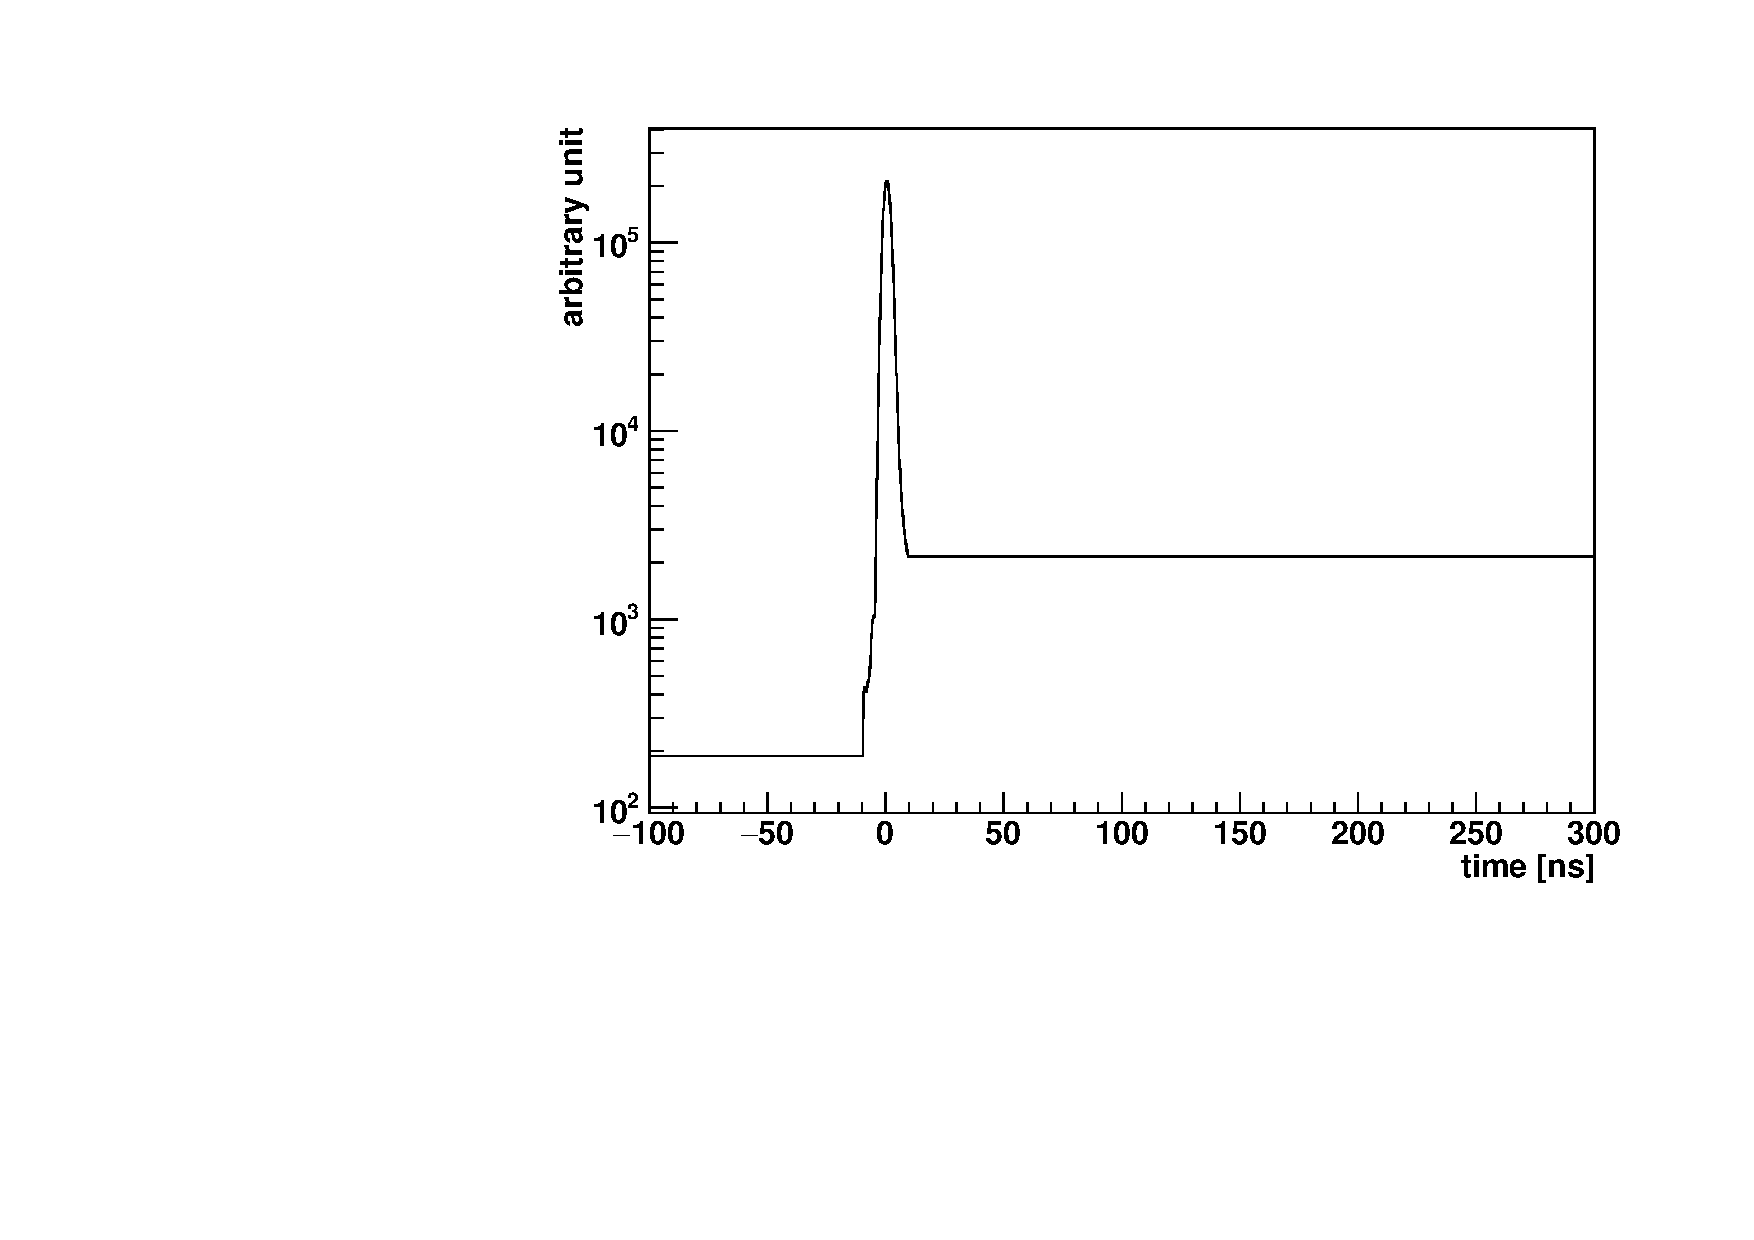
\includegraphics[width=10cm]{MPW_timingPDF.pdf}
	\caption{The PMT response time profile as the timing $PDF$ for the vertex reconstruction.}
	\label{fig:MPW_timingPDF}
\end{figure}

For a trial vertex $(\vec{X}_0,t_0)$, the fitter calculates a $t_{res}$ value with respect to each hit PMT. Looping over all the hit PMTs, a likelihood function is built as:
\begin{equation}\label{eq:vertexLogL}
\ln\mathcal{L}(\vec{X}_0,t_0)=\sum_{i=1}^{{\mathrm{NHits}}}\ln P(t^i_{res}),
\end{equation}
where $t^i_{res}$ is the time residual calculated from the $i^{th}$ hit PMT; NHits is the total number of the hit PMTs triggered by an event and $P(t^i_{res})$ is the probability returned by reading the $PDF$ when given a $t^i_{res}$ for the $i^{th}$ hit PMT.

Therefore, the likelihood function starts with a random ($\vec{X}_0,t_0$) as a seed and calculates the likelihoods and their derivatives for various paths assuming straight-line paths of the prompt Cherenkov light from the trial vertex $(\vec{X}_0,t_0)$ to each of the hit PMTs. The trial vertex is varied until the likelihood function reaches the global maximum when the best-fit vertex is found.

This fitting scheme is tackled by the Levenberg-Marquardt (MRQ) method, which is commonly used for fitting the nonlinear model with multiple parameters. This method is described in detail in the Sect.~\ref{appendix:MRQ} and its applications for the \texttt{MP fitter} framework are also described. Also see Refs.~\cite{gregory2005bayesian, press2007numerical} for details.

As will be shown in the following sections, one of the main tasks for the fitter is to calculate the $t_{transit}$ by evaluating light paths.  As mentioned at the beginning, the water phase geometry is the simplest situation. While in the other situations, the AV is filled with the wavelength shifter or scintillator. They are different materials with cavity water, making the light path calculations complicated.

\subsection{Direction Reconstruction}\label{sect:waterDirection}
A direction vector $\vec{u}$ can be determined by two parameters: the zenith angle $\theta$ and the azimuth angle $\phi$. Then in the Cartesian coordinate system, it can be written as: 
\begin{equation}
\vec{u}=(\cos\phi\sin\theta,\sin\phi\sin\theta,\cos\theta).
\end{equation}

\begin{figure}[htbp]
	\centering
	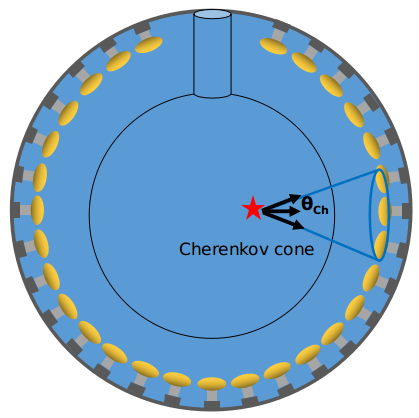
\includegraphics[width=6cm]{mpwDiagram2.png}
	\caption{Diagrams of position in the SNO+ water phase geometry.}
	\label{mpwdiagram_direction}
\end{figure}
To fit for the direction with 2 parameters: $\theta$ and $\phi$, similar to the vertex reconstruction, a random trial direction $\vec{u}_0(\phi_0,\theta_0)$ is generated by using \texttt{CLHEP}, see Sect.~\ref{appendix:random_gen}. The direction fitter then evaluates an angular parameter, $\cos\theta_{\mathrm{Ch}}$, which is the angle between $\vec{u}_{0}$ and $\vec{X}_{{\mathrm{diff}}}\equiv \vec{X}_{event}-\vec{X}_{PMT}$. Therefore, the direction fitter requires an event position as the input, and it goes after the vertex fitter\footnote{It has been discussed that, instead of going into two steps, the vertex and direction can be fit simultaneously by utilizing the MRQ algorithm for fitting six parameters ($x,y,z,t,\theta,\phi$). However, it shows that the results were worse by using this method.}.

An 1D $PDF$ is used for fitting the angular model, as shown in Fig.~\ref{fig:MPW_angularPDF}. This $PDF$ serves as a model of the angular distributions of the triggered PMTs to an event. It was obtained from 10000 MC simulations of 5-MeV $e^-$ events generated at the detector center ($\vec{X}_{MC}=(0,0,0)$), and traveling along the positive side of the x axis, i.e., the direction of the momentum is $\vec{u}_{MC}=(1,0,0)$\footnote{Here 5 MeV is a typical energy for the SNO+ water phase analysis. It shows that using the $PDF$s generated by the other $e^-$ energies does a minor effect on the reconstruction results.}.

\begin{figure}[!htb]
	\centering
	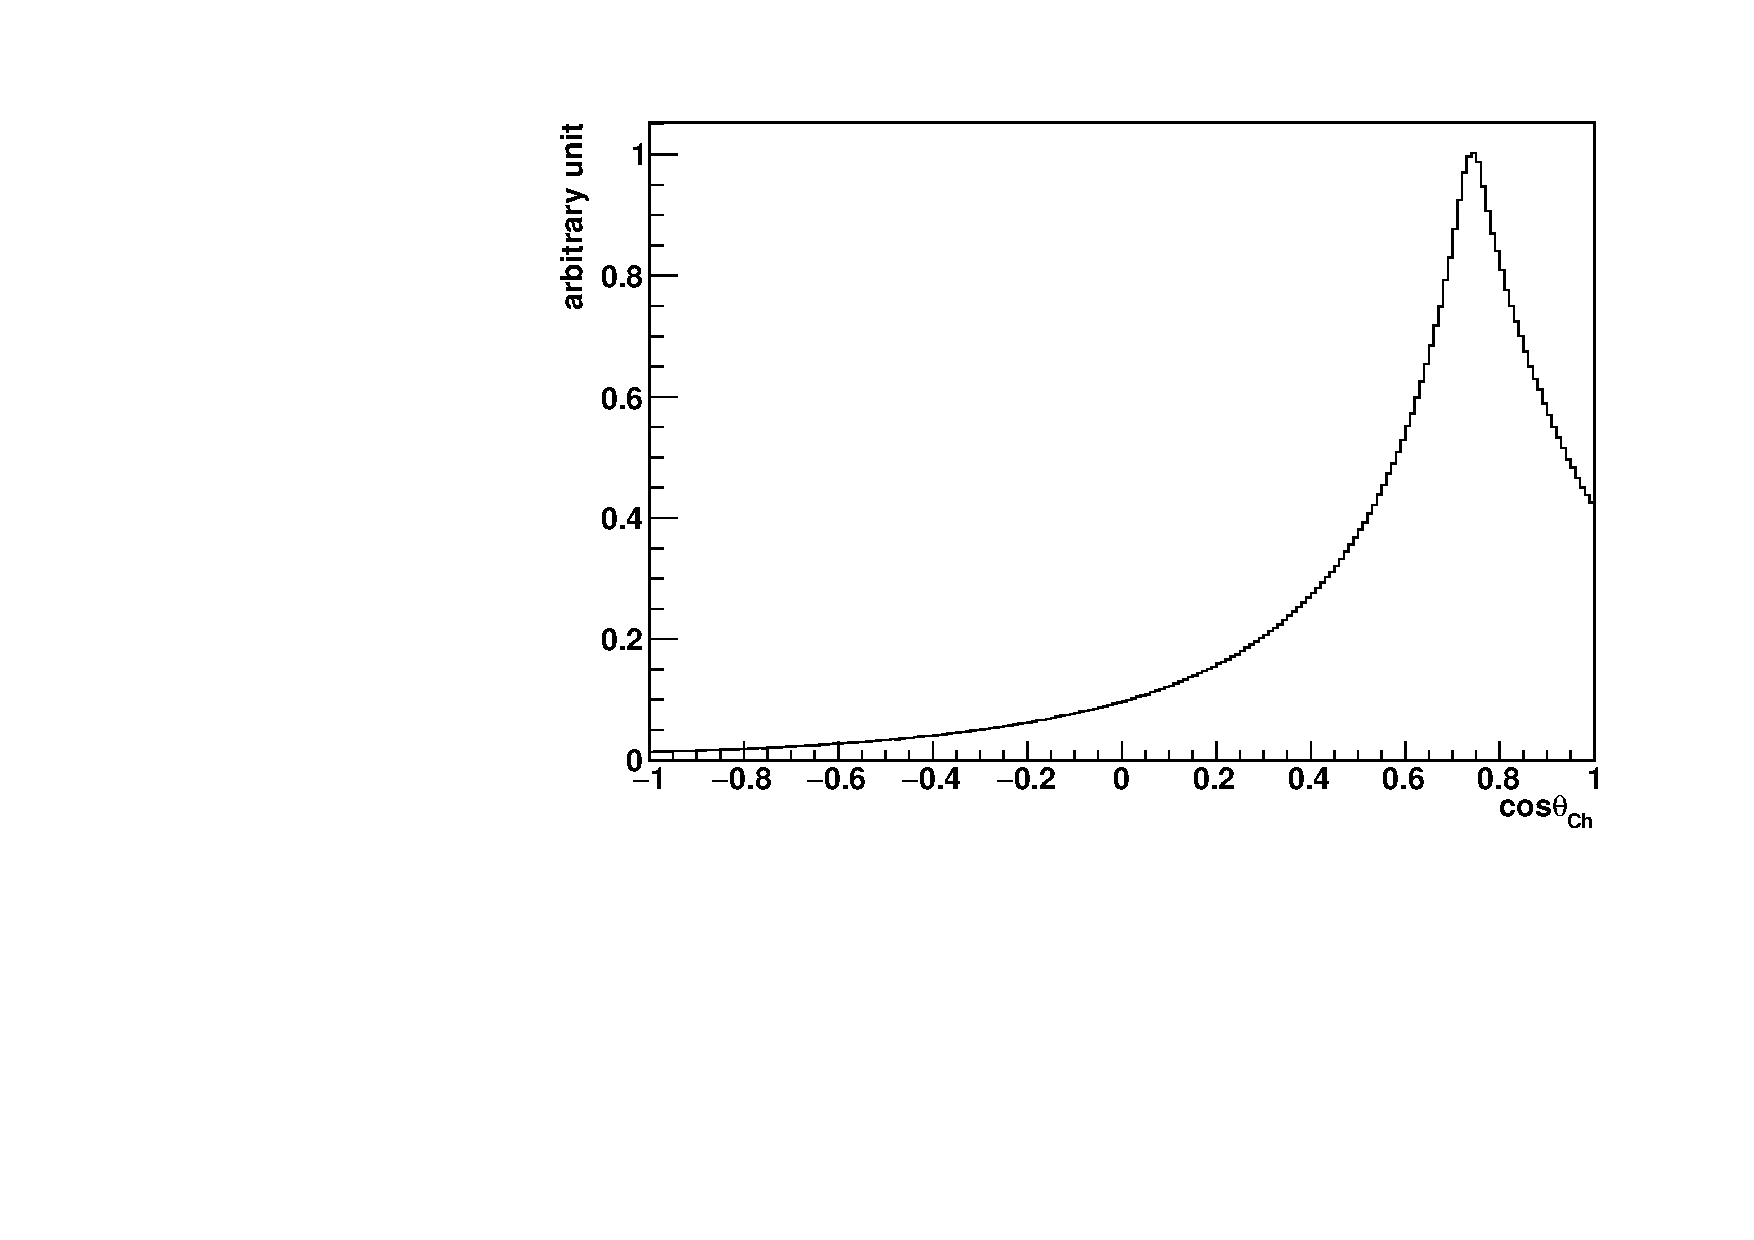
\includegraphics[width=10cm]{MPW_angularPDF.pdf}
	\caption{PMT angular distribution as the angular response $PDF$ for direction reconstruction.}
	\label{fig:MPW_angularPDF}
\end{figure}

For the $i^{th}$ hit PMT, $\cos\theta^i_{\mathrm{Ch}}=\vec{u}_0\cdot\frac{\vec{X}^i_{{\mathrm{diff}}}}{|\vec{X}^i_{{\mathrm{diff}}}|}$, then the likelihood function is built as:
\begin{equation}
\ln L(\vec{u}_0)=\sum_{i=1}^{{\mathrm{Nhits}}}L_i(\cos\theta_{\mathrm{Ch}}^i),
\end{equation}

Finally, the fitter fits for the angular $PDF$ by using the MRQ method to obtain the best-fit direction. There a few optimizations for improving the fitter performances. First, the group velocity used in the time of flight calculation is tuned, as shown in Sect.~\ref{sect:tuneGroupVelocity}. In Sect.~\ref{sect:fitterPull}, a drive correction for compensating the pulls in the reconstructed position is discussed. In Sect.~\ref{sect:PMTselector}, PMT selectors for sending proper PMT information to the fitter are discussed. 

\subsection{Effective Group Velocity}\label{sect:tuneGroupVelocity}
When photons travel through the detector, their group velocities ($v_{gr}$) change with different refractive indices of different detector materials. The group velocities also depend on the wavelengths of the photons: $v_{gr}=c/n(\lambda)$. Fig~.\ref{nVsWavelength} shows the measured refractive indices ($n$) as a function of wavelength, obtained from the measurements of laserball scans in the SNO+ water phase\cite{laserball_groupVelocity}. Furthermore, the $v_{gr}$ can change when the photons are scattered, absorbed, refracted and reflected in the detector.

\begin{figure}[!htb]
	\centering
	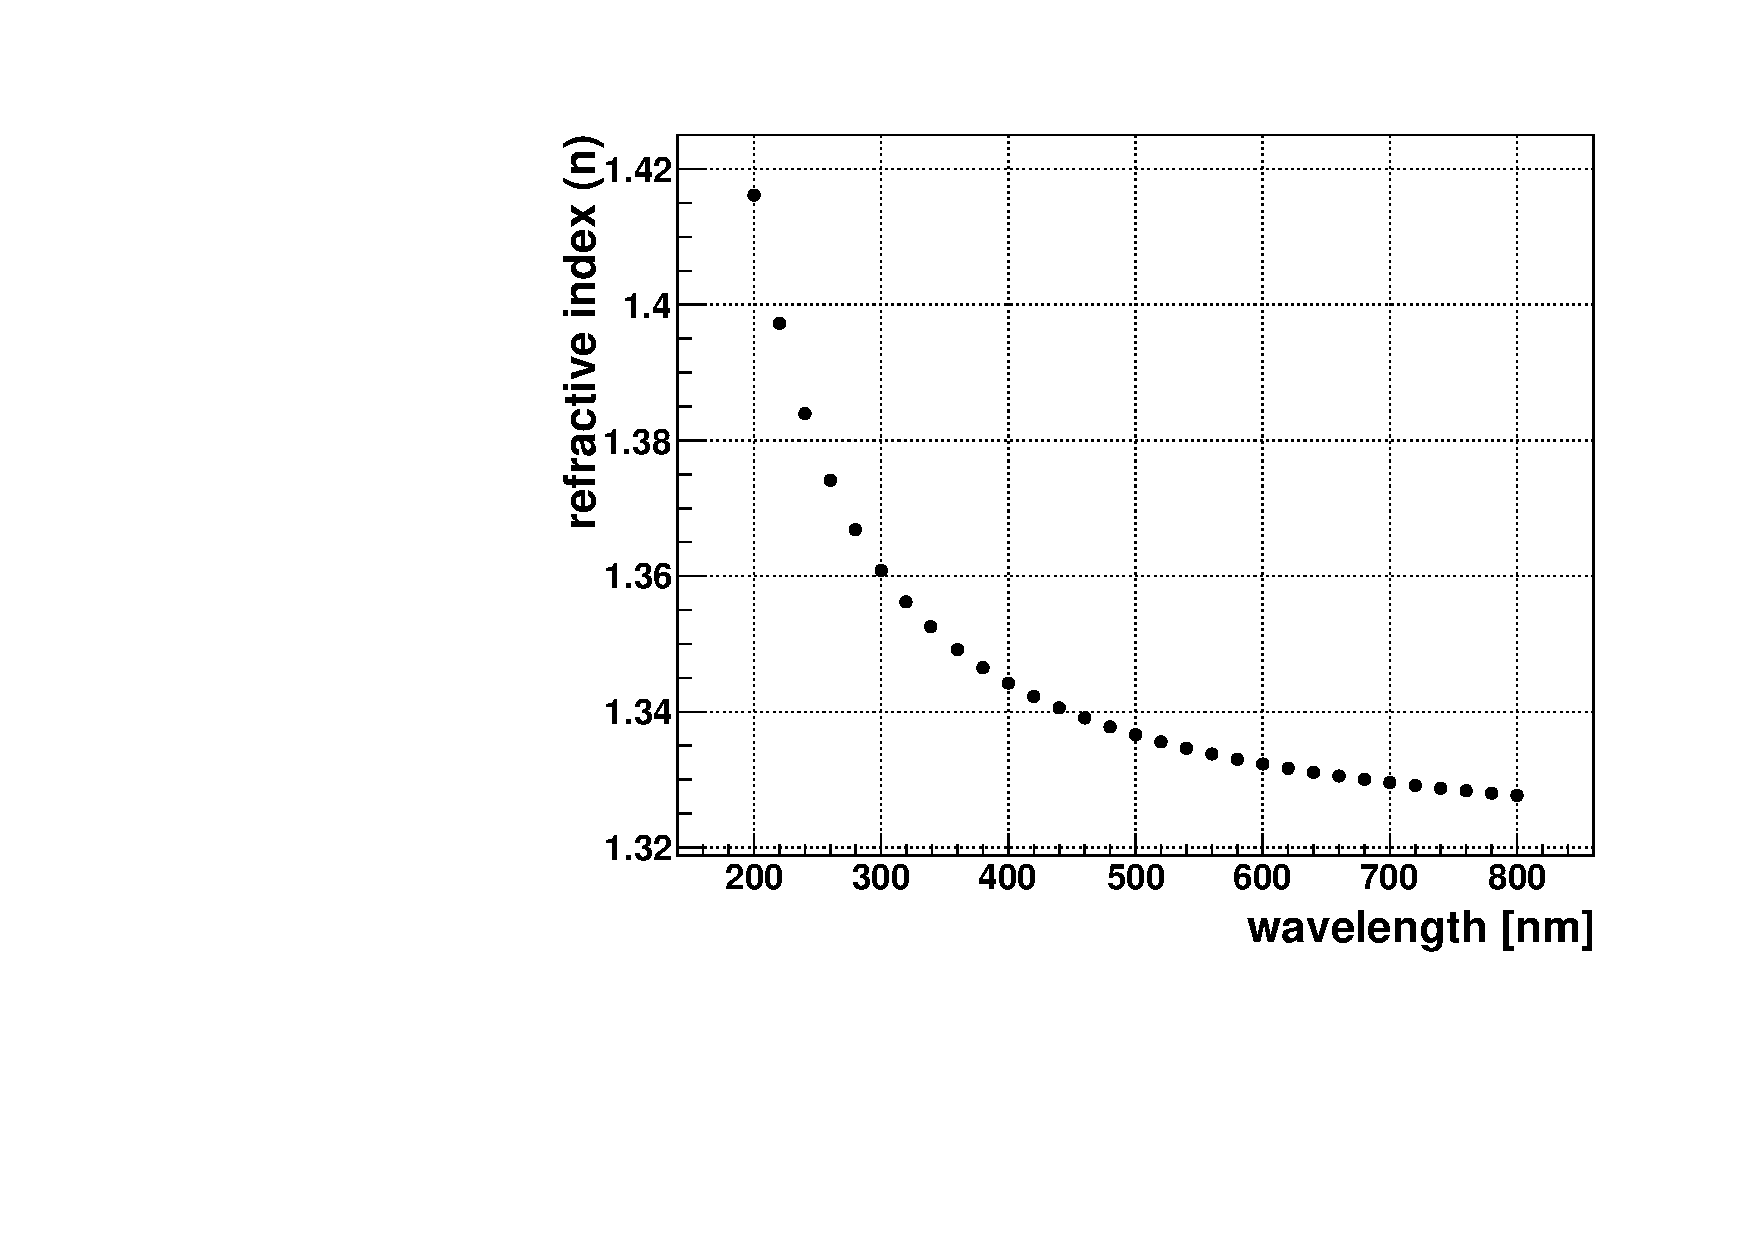
\includegraphics[width=6cm]{refractiveIndexVsWavelength.pdf}
	\caption[Refractive index vs wavelength.]{Refractive index vs wavelength. These values are based on the measurements from laserball calibration scans in the SNO+ water phase\cite{laserball_groupVelocity}.}
	\label{nVsWavelength}
\end{figure}

To simplify these complicated situations of $v_{gr}$ for the reconstruction, a tuned value of the $v_{gr}$ is used in the straight line light path calculation. As mentioned in Sect.~\ref{sect:mpw}, the water vertex fitter calculates the $t_{transit}$ by evaluating the distances from the trial vertex to the hit PMTs: $t_{transit}=|\vec{x}_{event}-\vec{x}_{PMT}|/v_{gr,eff}$, where the $v_{water}$ is replaced by the effective group velocity $v_{gr,eff}$. The value of the $v_{gr,eff}$ set in the fitter can introduce biases in the reconstructed position, which is mainly due to a ``complementary'' effect of the fitter. Setting a large value of $v_{gr,eff}$ (a fast effective group velocity) will decrease the $t_{transit}$, while according to Eqn.~\ref{eq:tres_define}, the $t_{res}$ will increase. During the reconstruction, when the fitter compares the large $t_{res}$ with the timing $PDF$, it will attempt to place the trial vertex away from the hit PMTs to increase the $t_{transit}$ and then decrease the $t_{res}$, as illustrated in Fig.~\ref{fig:effectiveVg}. On the other hand, if the $v_{gr,eff}$ is set too small (or too slow), the $t_{transit}$ will increase while the $t_{res}$ will decrease, and the fitter will place the trial vertex closer towards the hit PMTs to increase the $t_{res}$. These effects can be quantified as radial bias ($r_{bias}$), which is the difference between the reconstructed and true (MC) positions ($\vec{X}_{fit}-\vec{X}_{MC}$), projected along the radial component of the true position (the unit vector $\hat{X}_{MC}$)\cite{coulter2013modelling}:

\begin{equation}
r_{bias} \equiv (\vec{X}_{fit}-\vec{X}_{MC})\cdot \hat{X}_{MC},
\end{equation}

\begin{figure}[!htb]
	\centering
	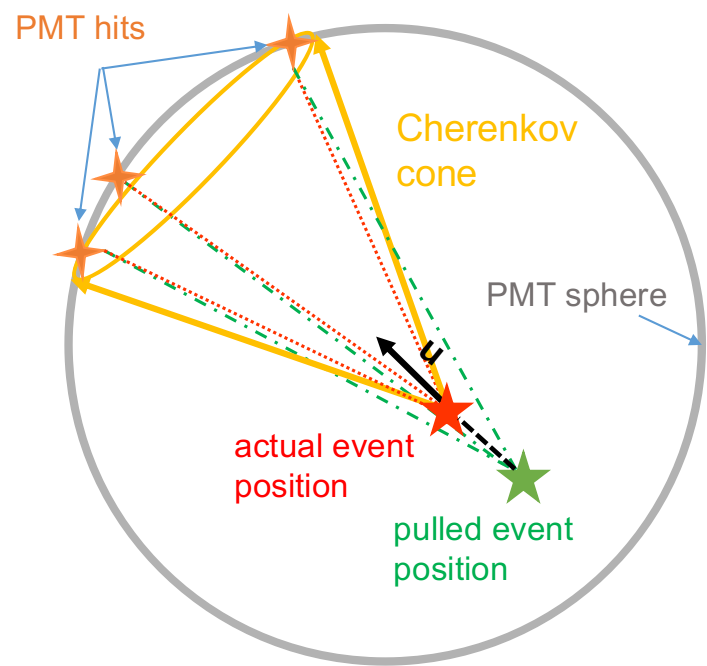
\includegraphics[width=6cm]{effectOfGroupVelocity.png}
	\caption{A cartoon shows effects of tuning the effective group velocity. In this case, the effective group velocity is faster than expected, the fitted position is dragged back along the direction to increase the time of flight.	\label{fig:effectiveVg}}
\end{figure}
It shows that an overestimated $v_{gr,eff}$ (too fast) brings a positive radial bias to the true event position while an underestimated one (too slow) brings a negative radial bias.

In practice, the $v_{gr,eff}$ is calculated by an effective refractive index $n_{eff}$ (or called $RI$ value): $v_{gr,eff}=c/n_{eff}$. To obtain a reasonable $v_{gr,eff}$ for the water-phase vertex fitter, my first attempt is to obtain the value from linear interpolation based on the MC simulations. First, 500 simulations of 5-MeV $e^-$ were generated uniformly inside the AV and with isotropic momentum directions. Then the \texttt{MPW fitter} reconstructed the same MC simulations by using 7 different values of $v_{gr}$, from 200 to 230 mm/ns (the $n_{eff}$ is from 1.50 to 1.30), with a step of 5 mm/ns. The distributions of radial bias from each reconstruction results were calculated and fitted with Gaussian functions. The mean values of these Gaussian fits were taken as the values of the $r_{bias}$, and they were plotted against the $v_{gr}$, as shown in Fig.~\ref{fig:plotVgr}. A linear fit was applied on these points and it gives $v_{gr,eff}=215.868\pm 5.585$ mm/ns ($n_{eff}=1.3888$) at the point where $r_{bias}=0$.

\begin{figure}[!htb]
	\centering
	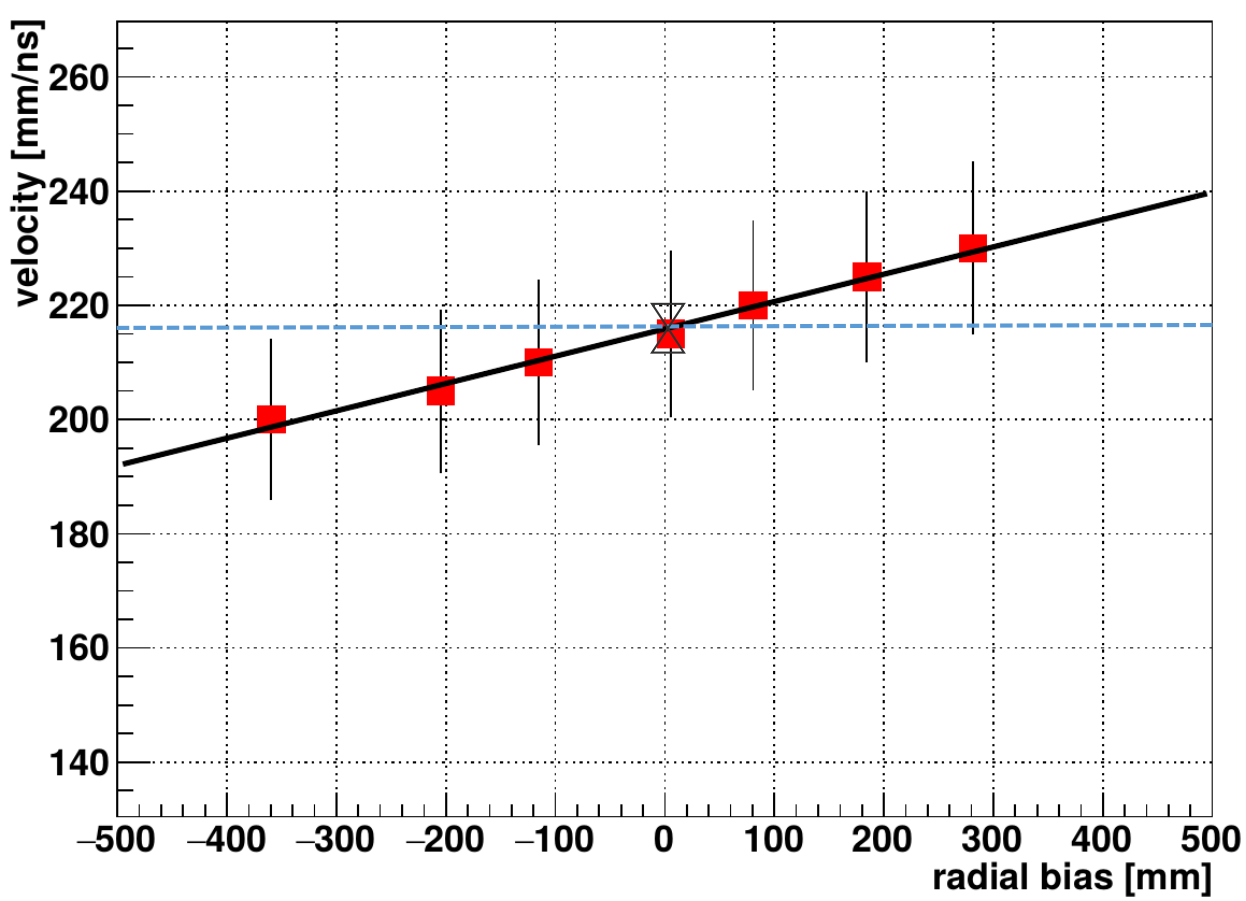
\includegraphics[width=6.5cm]{tune_groupVelocity_MPW.png}
	\caption[Group velocity vs. radial bias for the \texttt{MPW fitter}.]{Group velocity vs. radial bias for the \texttt{MPW fitter}.	\label{fig:plotVgr}}
\end{figure}

Later I turned to a more data-driven approach rather than tuning from the simulations. This approach is to extract an average group velocity by analyzing the $^{16}$N calibration source data. As shown in Fig.~\ref{n16_groupVeloctiy}, for the $^{16}$N central run-100934 and run-107055, the source was deployed almost at the PSUP center where the optical photons were created and propagated to reach the PMTs on the PSUP. 

For each event, it supposes that the triggered PMTs were found within a solid angle $\Omega=\pi(L/2)^2/r^2_{PSUP}$, where $L$ is the line segment and $r_{PSUP}=8390$ mm is the radius of the PSUP, as shown in Fig.~\ref{fig:n16_groupVeloctiy}. Since the diameter of the PMT concentrator is 27 cm, the line segment is chosen as $L = 50$ cm ($\theta=\arcsin(\frac{1}{2}L/r_{PSUP})\approx 0.17^\circ$) to let roughly 2 PMTs be within the $\Omega$. Then the arrival time $T_1$ was found by calculating $|\vec{X}_{source}-\vec{X}_{PMTin\Omega}|/v_{water}$, where $v_{water}=217.554$ mm/ns is an effective velocity obtained by the SNO+ for light water\cite{coulter2013modelling}.

\begin{figure}[!htb]
	\centering
	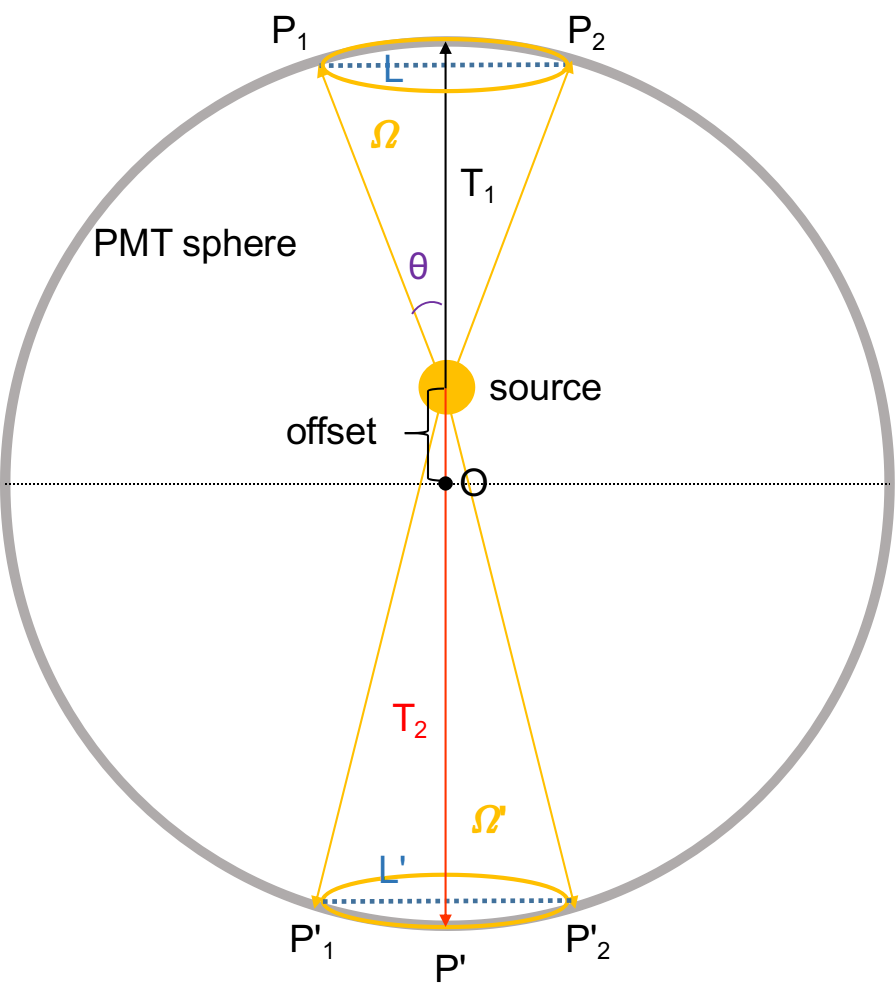
\includegraphics[width=6cm]{n16_groupVelocity.png}
	\caption{$^{16}$N central run for evaluating the average group velocity.}
	\label{fig:n16_groupVeloctiy}
\end{figure}

On the other hand, a solid angle $\Omega'$ is calculated as opposed to the $\Omega$ from the source position. Similarly, the triggered PMTs within the $\Omega'$ were found and then the arrival time $T_2$ is calculated. Thus the average group velocity was calculated as:
\begin{equation}
v_{gr}=\frac{2 r_{PSUP}}{(T_1+T_2)}.
\end{equation}

The final number of the $v_{gr}$ was calculated by averaging the $v_{gr}$ obtained from all the events and triggered PMTs in both the run-100934 and 107055. It finds the $v_{gr}=c/n_{water,eff}=216.478$ mm/ns, where $n_{water,eff}=1.38486$.

The SNO+ collaboration used a more complicated approach to measure actual group velocities in the SNO+ water detector by analyzing a set of laserball calibration runs\cite{groupVmeasure,anderson2021optical}. This analysis can give a more accurate $v_{gr}$, while it was not applied here.

For the vertex fitters used in the partial-fill and scintillator phases, since no internal calibration was performed, I adopt the linear interpolation method. It will be discussed in Sect.~\ref{sect:scintFitter}.

\subsection{Fitter Pull and Drive Correction}\label{sect:fitterPull}

An effect of ``fitter pull'' in the event vertex reconstruction utilizing the Cherenkov light was observed in the SNO experiment. The distribution of $(\vec{X}_{fit}-\vec{X}_{MC})/|\vec{X}_{fit}-\vec{X}_{MC}|\cdot \vec{u}_{fit}$ shows a large peak at +1, which indicates that the fitted position $\vec{X}_{fit}$ is prone to be pulled forward from the true position systematically along the event direction$\vec{u}$\cite{driveCorPeter,brice1996monte,coulter2013modelling}. 

Similar to the SNO heavy water case, in the SNO+ ultrapure water, Cherenkov photons created by an event trigger most of the PMT-hits with early timing and these hits are located within the Cherenkov cone; for the same event, there are also a few PMT-hits with later timing. These PMT hits can be caused by the scattered or reflected photons and they are located throughout the detector. For a random PMT hit, it is more probable to be placed outside the Cherenkov cone due to the geometry: consider an event happens at the center of the PSUP, the Cherenkov cone it produced will intersect the PSUP by an area of $2\pi R^2_{PSUP}(1-\cos41^\circ)$, which occupies about 12\% of the total area of the PSUP sphere. Therefore, for a random PMT-hit on the PSUP sphere, it has more than 88\% of chance to be placed outside the Cherenkov cone. 

For these later timing PMT hits, a similar ``complementary'' effect mentioned in Sect.~\ref{sect:tuneGroupVelocity} can also happen. When the fitter fits with $t_{res}$, for the large $t_{res}$ values caused by the later timing hits, it pulls the trial position away from the later timing hits to increase $t_{transit}$ and decrease $t_{res}$, as illustrated in Fig.~\ref{fitterPull}. This effect was also explained as ``straighten out delayed photons'' by the timing fitter in \cite{driveCorPeter}. Furthermore, the major early hits can also cause small $t_{res}$ values and thus the fitter pulls the trial position closer towards the early hits to decrease $t_{transit}$ and increase $t_{res}$. Recall that the early hits are located on or around the Cherenkov cone, therefore an overall effect of this ``fitter pull'' is that the fitted position will be pulled along the axis of the Cherenkov cone and towards the PSUP sphere. This pull direction is coincident with the event direction.

\begin{figure}[!htb]
	\centering
	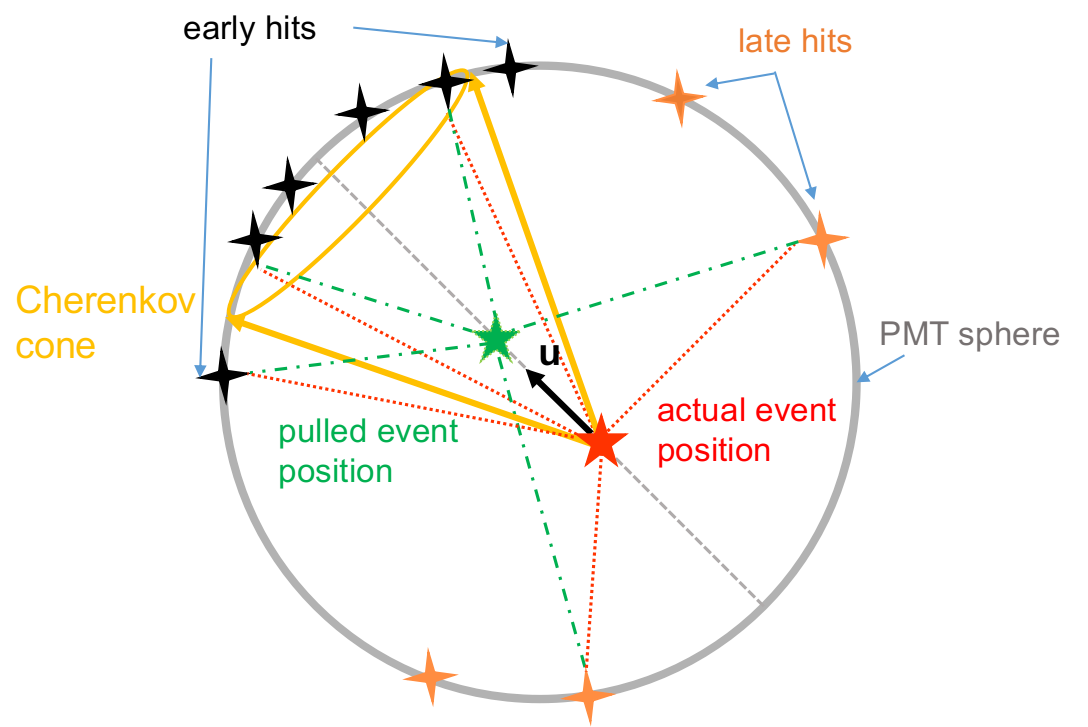
\includegraphics[width=8cm]{fitterPull.png}
\caption[A cartoon shows fitter pull effect.]{A cartoon shows fitter pull effect, modified from Fig.~C.2 in Ref.~\cite{brice1996monte} and Fig.~2,3,4 in Ref.~\cite{driveCorPeter}.}
	\label{fitterPull}
\end{figure}

A simple way to eliminate this ``fitter pull'' effect is to pull back the fitted event position against the event direction. This is called ``drive correction''.   

Once the \texttt{MPW fitter} obtains both of the fitted position and direction, the drive correction is applied on the fitted position by $\vec{X}_{\mathrm{corrected}} = p_0\vec{X}_{fit}+p_1\vec{u}_{fit}$, where $p_0$ and $p_1$ are the correction parameters, as shown in Fig.~\ref{drivecor}.
\begin{figure}[!htb]
	\centering
	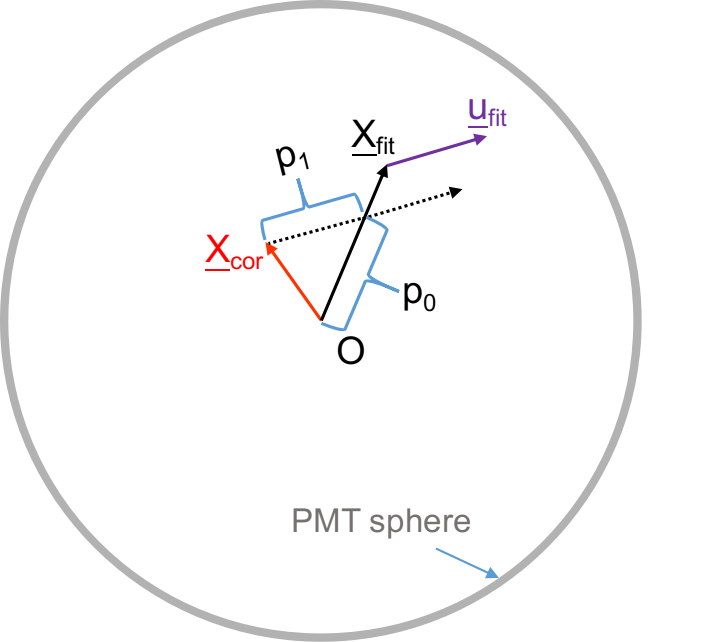
\includegraphics[width=6cm]{driveCor.png}
	\caption{ A diagram illustrates the drive correction.}
	\label{drivecor}
\end{figure}

To obtain the values of $p_0$ and $p_1$, I generated $e^-$ events distributed isotropically inside the AV. The simulations with various $e^-$ energies from 2 to 10MeV by an 1MeV step were produced. Then the \texttt{MPW fitter} was applied on each simulations and returned the results of $\vec{X}_{fit}$ and $\vec{u}_{fit}$. Taking the Monte Carlo generated positions $\vec{X}_{MC}$ as the true positions, for all the fitted events, a $\chi^2$ function is calculated by:
\begin{equation}
\chi^2 = \sum_{i=1}^{N_{\mathrm{events}}}[\vec{X}^i_{MC}-(p_0\vec{X}^i_{fit}+p_1\vec{u}^i_{fit})]^2,
\end{equation}

The $p_0$ and $p_1$ are obtained by minimizing the $\chi^2$ function. When calculating the $\chi^2$, the fitted events of $|\vec{X}_{fit}-\vec{X}_{MC}|>3~m$ are thrown away to improve the $\chi^2$ minimization results.

For the 2 to 10-MeV $e^-$ event simulations (using \texttt{RAT} version 6.17.6), the obtained values of $p_0$ and $p_1$ are energy or NHit dependent. However, it does not improve the results if using the NHits dependent functions $p_0$(NHit) and $p_1$(NHit) as drive corrections.
Finally we take the average values from the 5 to 10 MeV electrons simulations and the drive correction is set as: 
\begin{equation}
\vec{X}_{\mathrm{corrected}} = 0.9868\vec{X}_{fit}+(-78.417)\vec{u}_{fit}.
\end{equation}

Note that these drive correction parameters were obtained from simulations and changes of the simulation model, especially the optical model of the detector, can affect the $n_{gr,eff}$, mode cut and time residual cut, and then affect the drive correction parameters. However, the drive correction parameters can be re-coordinated with the changes in the simulation.

\begin{figure}[!htb]
	\centering
	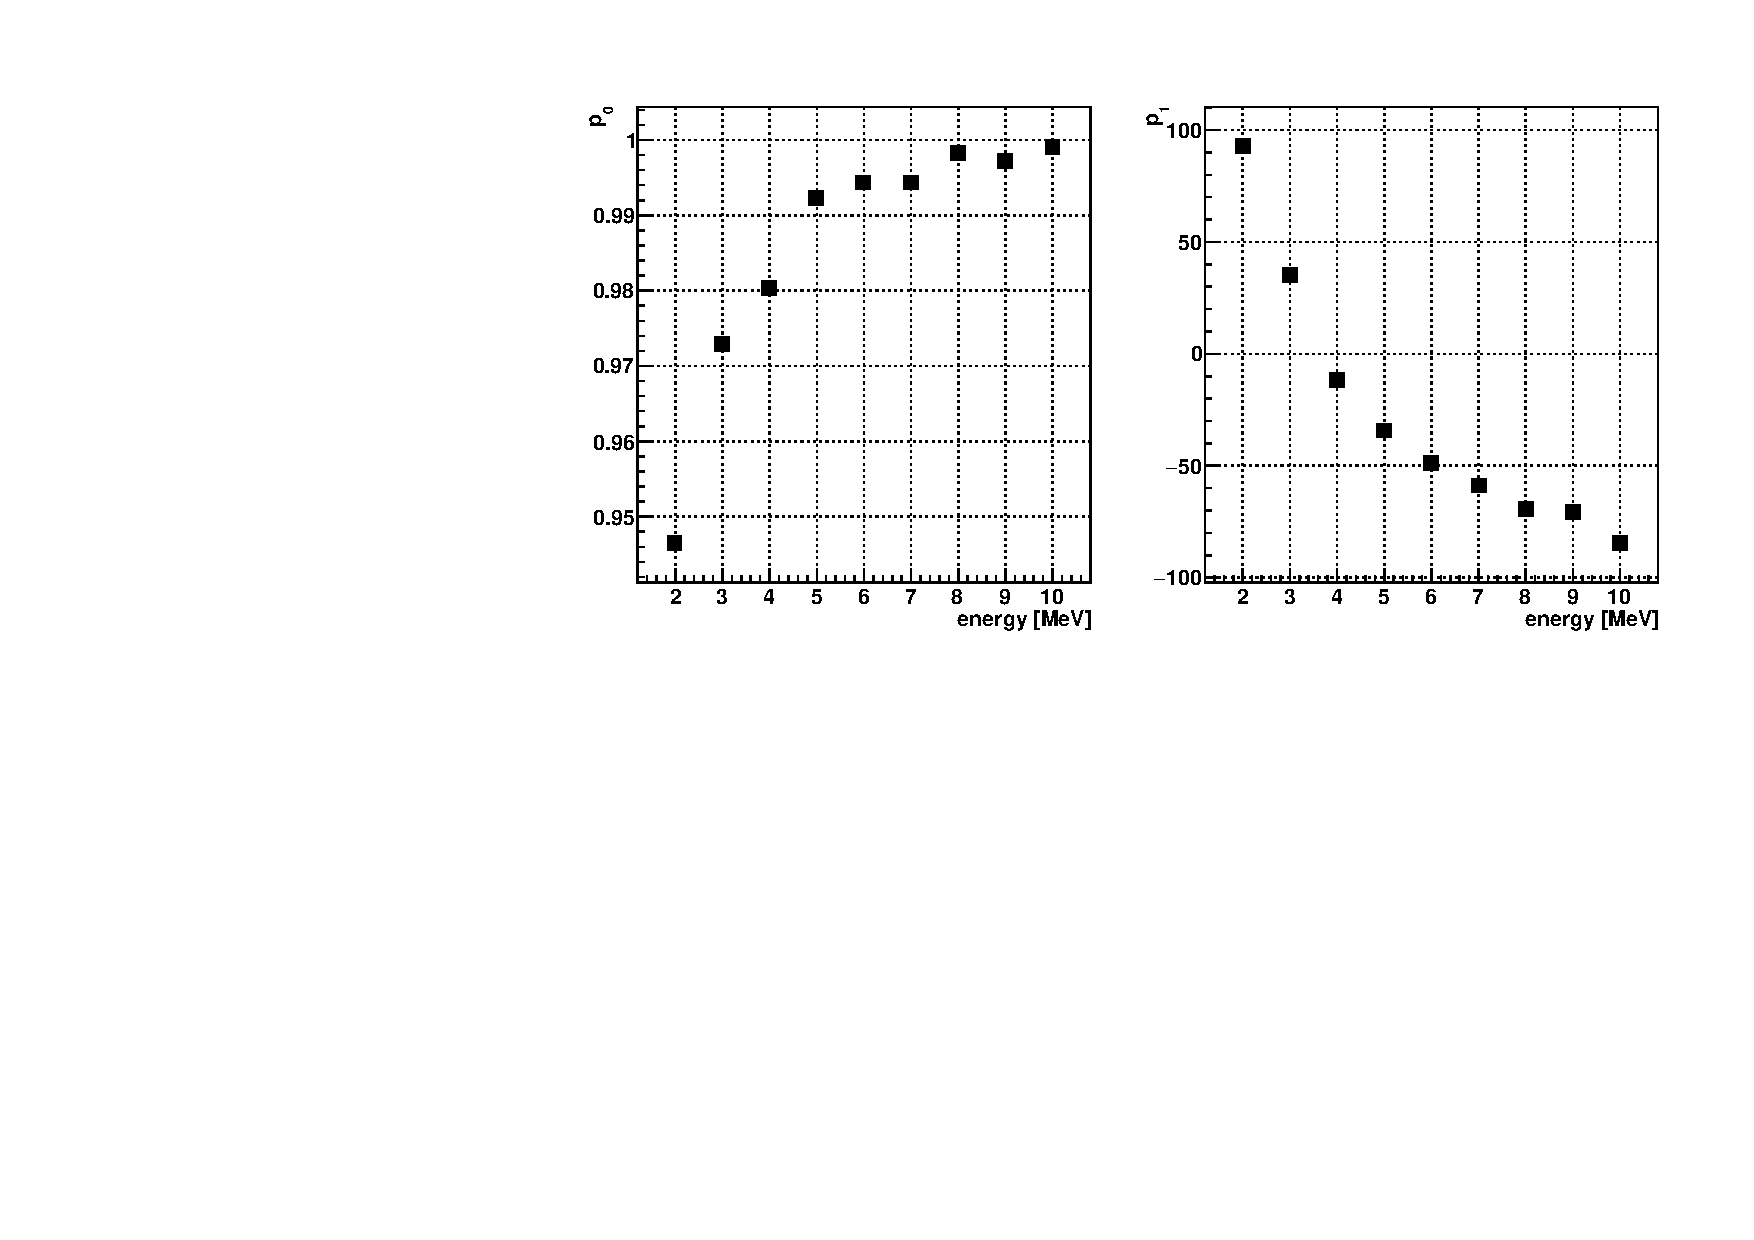
\includegraphics[width=10cm]{pullParVsEnergy.pdf}
	\caption{Drive correction parameter $p_0$ (left) and $p_1$ (right) as a function of energy.}
	\label{pullParVsEnergy}
\end{figure}

To check the effects of the drive correction, 1000 simulations of the 5-MeV $e^-$ were generated at the detector center with momentum direction at (1,0,0). It shows that the drive effect in the reconstruction causes a +50 mm bias from the detector center in the x axis (i.e., the pull in +x). The drive correction reduces this pull down to $\sim$+0.2 mm in the x axis. The resolution of the $r_{bias}$ distribution is also improved by $\sim$20 mm. With the same simulation settings, various energies of $e^-$ from 2 to 10 MeV (with a 1-MeV step) were generated to check the effects before and after the drive correction, as shown in Fig.~\ref{drivecorVsEnergy}. The pull is quantified by the radial bias mentioned in Sect.~\ref{sect:tuneGroupVelocity}. The distributions of the $r_{bias}$ in each simulation were fitted with Gaussian functions, and the Gaussian means were used as the pull. It shows that, with higher energy, the pull effect is larger. The drive corrections correct the radial biases by about 55 mm. The drive correction is also applied in the \texttt{Rat water fitter}, and their results are also shown.
\begin{figure}[!htb]
	\centering
	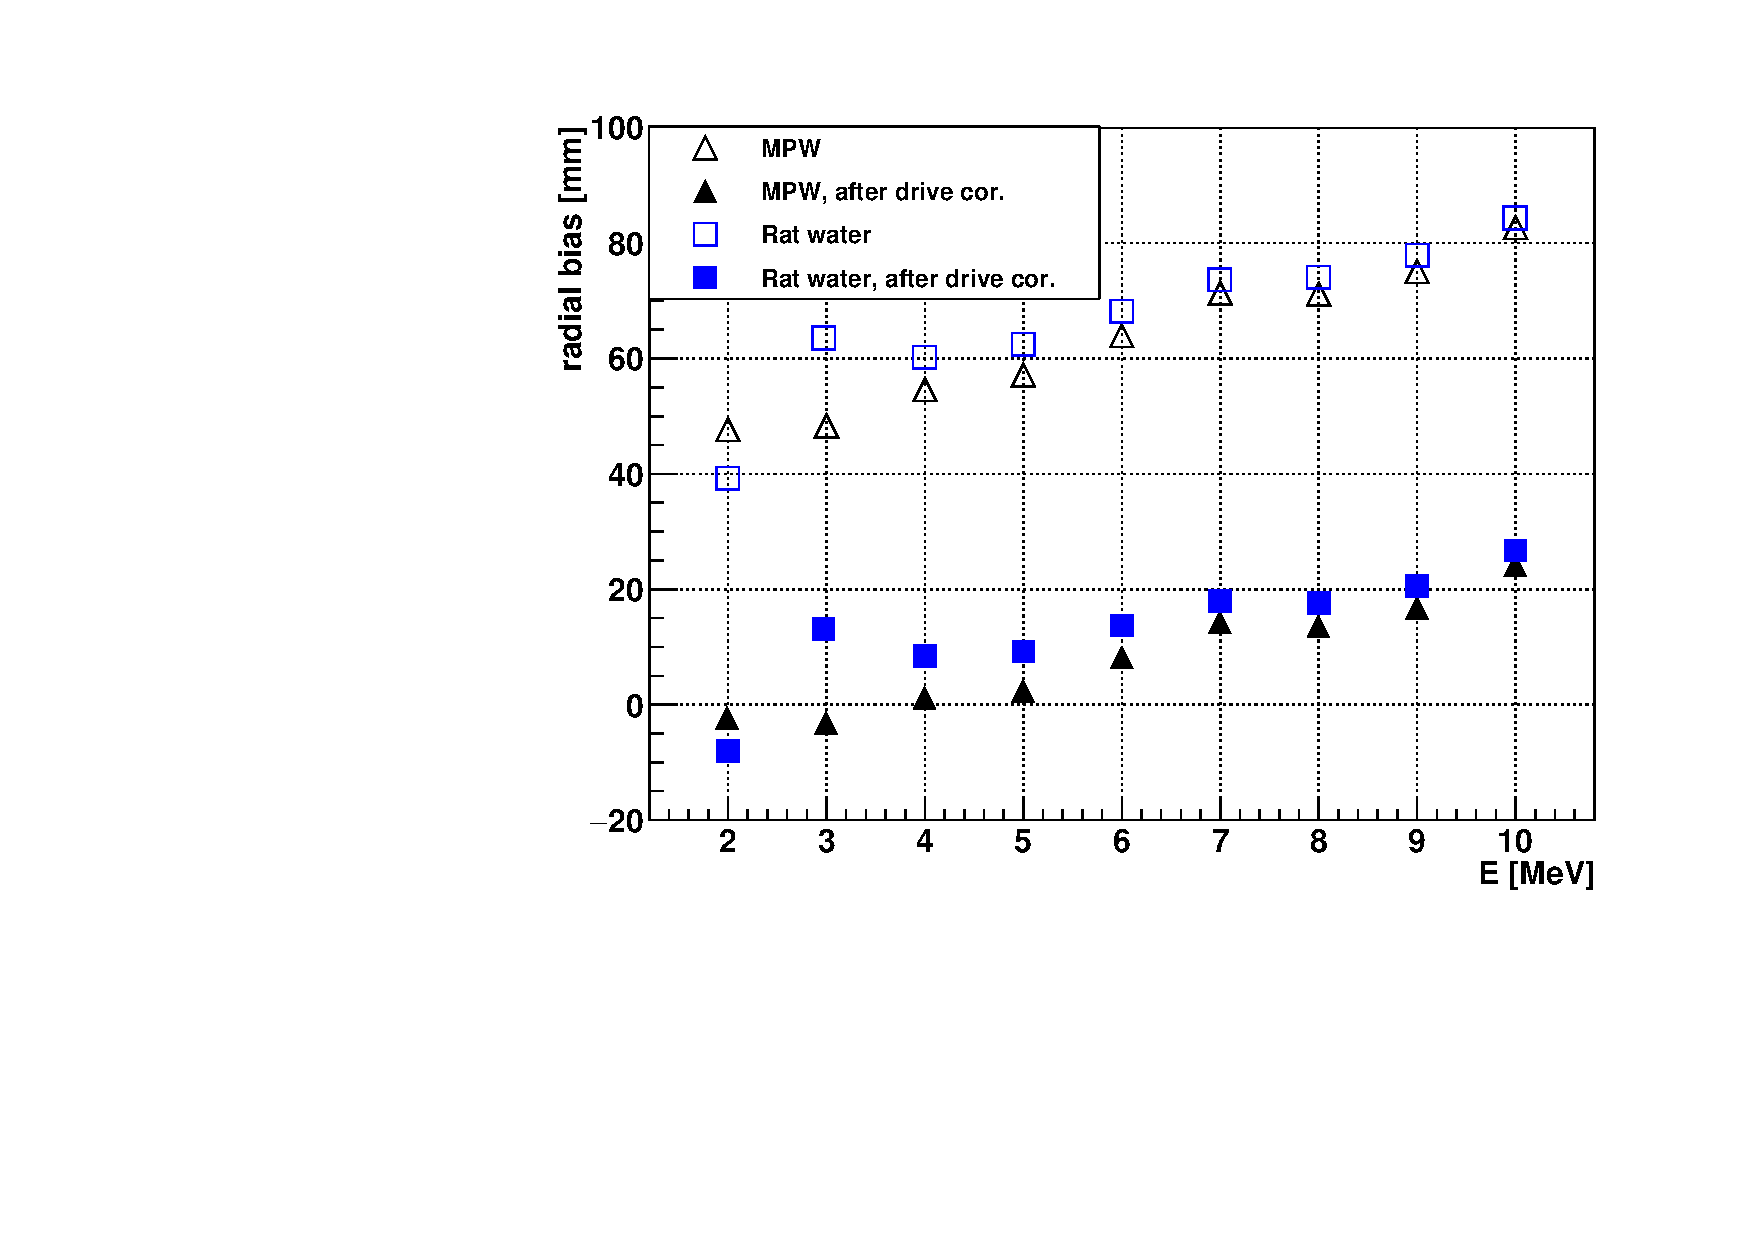
\includegraphics[width=9cm]{pullEffectVsEnergy.pdf}
	\caption[Radial biases of the simulated $e^-$ events as a function of energy.]{Radial biases of the simulated $e^-$ events before (unfilled triangles) and after the drive correction (filled triangles), as a function of energy. The results from the official \texttt{RAT water fitter} are also shown here, with the unfilled blue squares for biases before the correction and filled ones after the correction.}
	\label{drivecorVsEnergy}
\end{figure}

\subsection{PMT Selectors for the Reconstruction}\label{sect:PMTselector}
PMT selectors were developed to selecting proper PMTs for the reconstruction algorithm from all the recorded PMTs triggered by an event. The purpose is to optimize the fitter results and boosting up the fit speed. The PMT selectors used by the \texttt{MP fitter} are:

\begin{itemize}
	\item[$\bullet$] Straight Light Path Time Residual Cut Selector
	
	This selector is used for the direction reconstruction for the SNO+ water phase. It was first developed by Kalpana Singh\cite{kalpanaMPFitter}. In the selector, the value of time residual ($t_{res}$) is calculated for each hit PMTs from an event and the PMT returning a $t_{res}$ value within the prompt time window of $[-10.0, 120.0]~ns$ is selected for the fitter. The selector calculates the $t_{res}$ by using straight line light paths, which is the same as the \texttt{MPW fitter}. The selector mostly removes the PMTs triggered by late timing photons, such as the photons reflected off the detector elements (called ``late light''), and then keeps the possible Cherenkov ring hit pattern clear for the direction reconstruction. Removing the irrelevant PMTs can potentially boost up the fit speed.
	
	\item[$\bullet$] Mode Cut Selector
	
	This selector was developed by the SNO+ collaboration for all fitters. It checks the hit time ($t_\mathrm{PMT}$) distributions of all the hit PMTs and finds a mode value of the hit time ($t_{mode}$). If $t_{mode}$ fails to be found, it calculates a median value ($t_{median}$) instead\cite{modeCut}. Then it selects the PMT with $t_\mathrm{PMT} \in [t_{mode}+t_{low}, t_{mode}+t_{high}]~ns$. This selector is used to remove the PMTs triggered by noise and light light from reflection. The values of $t_{low},~t_{high}$ are optimized for different scintillators. For the \texttt{MPW fitter}, I found that the optimized window is $[t_{mode}-50, t_{mode}+100]$ ns by checking with the fit biases and resolutions for the \isotope[16]{N} central run data in the water phase, while for the \texttt{MP scint-water} and \texttt{scint fitter} the optimized window is $[t_{mode}-100, t_{mode}+100]$ ns based on checking with the simulations.
	
	\item[$\bullet$] Uniform PMT Selector
	
	I implemented this selector and the Earliest Hit Selector mentioned below for the partial-fill and scintillator phases when a single event can trigger many PMTs due to high light yields of the liquid scintillator. In this case, the fit speed for each event becomes slow, which can challenge the data processing. These selectors can reduce the number of the hit PMTs to a designated number ($n_{select}$) to boost up the fit speed while still keep acceptable results of the fit bias and resolution. 
	
	For the Uniform PMT Selector, when an event triggers $N$ calibrated PMTs, the selector goes through these recorded PMTs and uniformly picks up one PMT by an interval of $\left \lceil{N/n_{select}}\right \rceil $. If $N\leq n_{select}$, the selector does nothing. By doing this, the selector uniformly reduces the number of the PMTs for the fitter without an obvious bias.
	
	\item[$\bullet$] Earliest Hit PMT Selector
	
	This selector first groups the PMTs by their positions in the PSUP sphere. Taking the centre of the sphere as the origin of the coordinate, the sphere is divided by the azimuth angle $\phi$ (as longitude) and zenith angle $\theta$ (as latitude). The PMT positions are projected to $\phi\in [-\pi,\pi]$ and $\cos\theta\in [-1, 1]$ on the sphere, each is uniformly divided into $n$ intervals. Thus, the PMTs are grouped into $n\times n$ panels by $\phi$ and $\cos\theta$: $\mathrm{PMT}(\phi_i,\cos\theta_j) \in [i\cdot\phi/n, j\cdot\cos\theta/n],~(i,j=1,2,..,n)$, see Fig.~\ref{GroupPMTs}. 
	\begin{figure}[!htb]
		\centering
		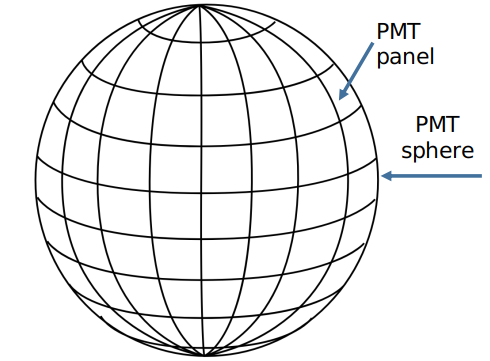
\includegraphics[width=5cm]{GroupPMTs.png}
		\caption{The PMTs are grouped by dividing the PSUP sphere with latitudes and longitudes.}
		\label{GroupPMTs}
	\end{figure}
	
	In each panel, the selector first removes the hit PMTs which are triggered too early ($t_\mathrm{PMT}<100~ns$, where $100~ns$ is set as a default threshold). These PMTs could be triggered by noises, such as the pre-pulsing from thermal noises. Then in the rest of the hit PMTs, the selector picks up one PMT which has the earliest $t_\mathrm{PMT}$ in the panel. Thus the number of the hit PMTs is reduced to $n\times n$ for the fitter, i.e., $n_{select}=n\times n$. If $\mathrm{NHits}\leq n_{select}$, the selector does nothing. 
	
	The other timing parameters can also be used for selecting the PMT in each panel, such as the $t_{mode}$ or the $t_{median}$. However, tests on the simulations for the scintillator phase show that using the earliest hit time $t_\mathrm{PMT}$ gives fewer fit biases and better fit resolutions.
	
	Tests on the 10-MeV $e^-$ simulations in the scintillator phase show that applying this selector with $n_{select}=16\times16$, the fit speed was reduced from 1.2 s/event to 0.4 s/event.
\end{itemize}

\subsection{Position Figure of Merit}\label{sect:positinFoM}
A quantity called scaled $\log L$ ($scaleLogL$) is used as the position reconstruction FoM ($posFoM$): $scaleLogL = \ln L/\mathrm{NHit}_{selected}$. This quantity utilizes the best log-likelihood returned by the \texttt{MP fitter} for a successfully reconstructed event vertex, and then it is scaled by the ``selected'' NHit ($\mathrm{NHit}_{selected}$), which is the number of the PMTs actually used by the fitter for the event vertex reconstruction, after the PMT selections mentioned in Sect.~\ref{sect:PMTselector}. This $posFoM$ quantity can remove a few mis-reconstruct events and then improve the results of the reconstruction.

\subsection{Performances of the Water Vertex Reconstruction}\label{sect:waterFitterVertex}

By using the \texttt{RAT} (version 6.17.6) package, simulations of 10000 $e^-$ events were generated at the detector center (in the PSUP coordination) with isotropic directions, i.e., the event momentum directions were generated randomly and uniformly over all directions. Default detector trigger settings in the SNO+ water phase were used (\texttt{N100Hi}=21.0, \texttt{N100Med}=16.0 and \texttt{N100Lo}=11.0). With these settings, some events may fail to trigger the detector, especially those with lower energies ($E<3$ MeV), and thus the number of the reconstructed events can be lower than the simulated events.

The average fit speed of the event vertex reconstruction for the 5-MeV $e^-$ simulations is 0.005 second/event and the direction reconstruction is 0.002 second/event, which are very fast and acceptable for the data processing in the SNO+ water phase. Fig.~\ref{fig:5MeVbeta_center_water} shows the position reconstruction results and performances for the 5-MeV $e^-$ events. The biases between the fitted and MC positions: $\vec{X}_{fit}-\vec{X}_{mc}=(x_{fit}-x_{MC},y_{fit}-y_{MC},z_{fit}-z_{MC})$, were projected on the x, y, and z axes respectively and their distributions were fitted with Gaussian functions. The mean of the fitted Gaussian ($\mu$) is taken as the fit position bias while the Gaussian sigma ($\sigma$) is taken as the fit position resolution.
\begin{figure}[htbp]
	\centering \label{fig:5MeVbeta_center_water}
	\subfigure[$x_{fit}-x_{mc}$]{
		\begin{minipage}[t]{0.5\textwidth}
			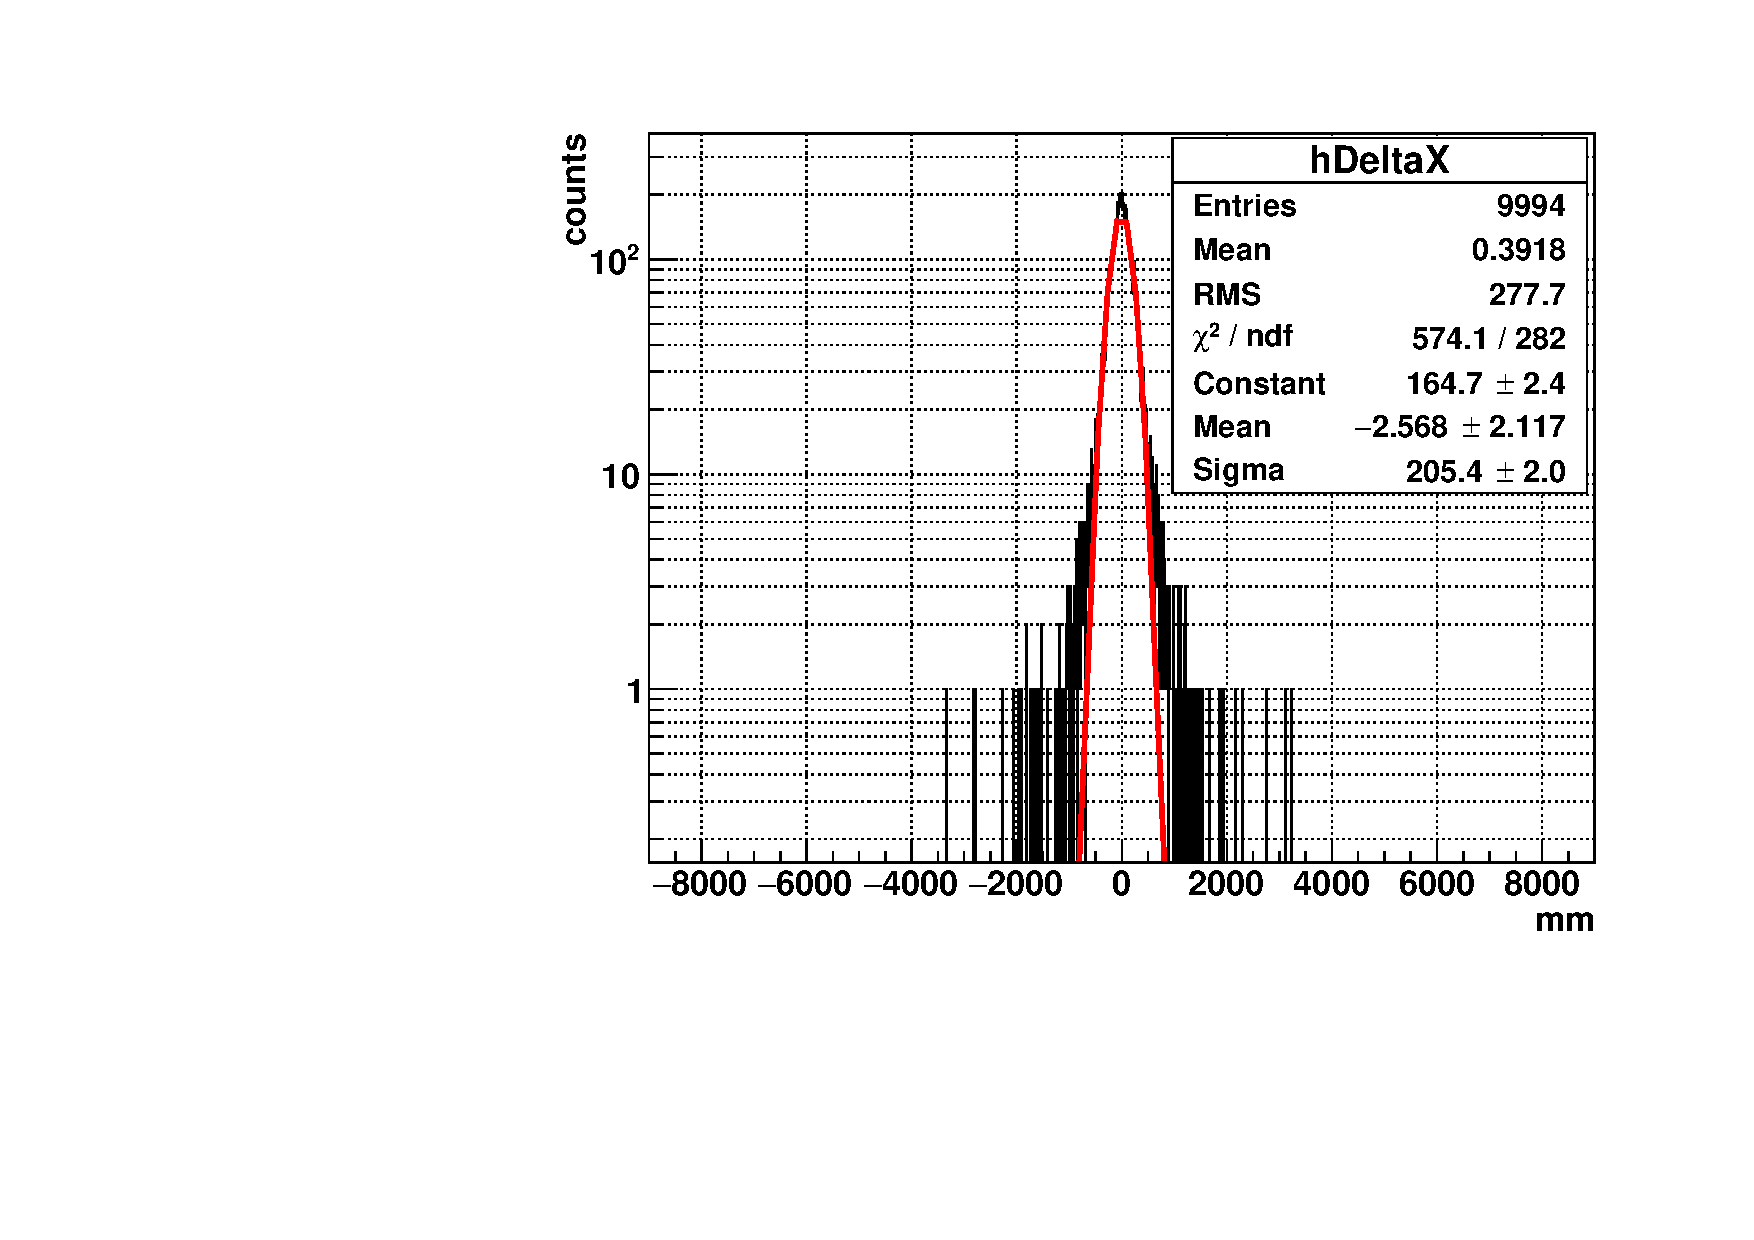
\includegraphics[width=8cm]{5MeVbetaX.pdf}
		\end{minipage}
	}   
	\subfigure[$y_{fit}-y_{mc}$]{ 
		\begin{minipage}[t]{0.4\textwidth}
			\centering
			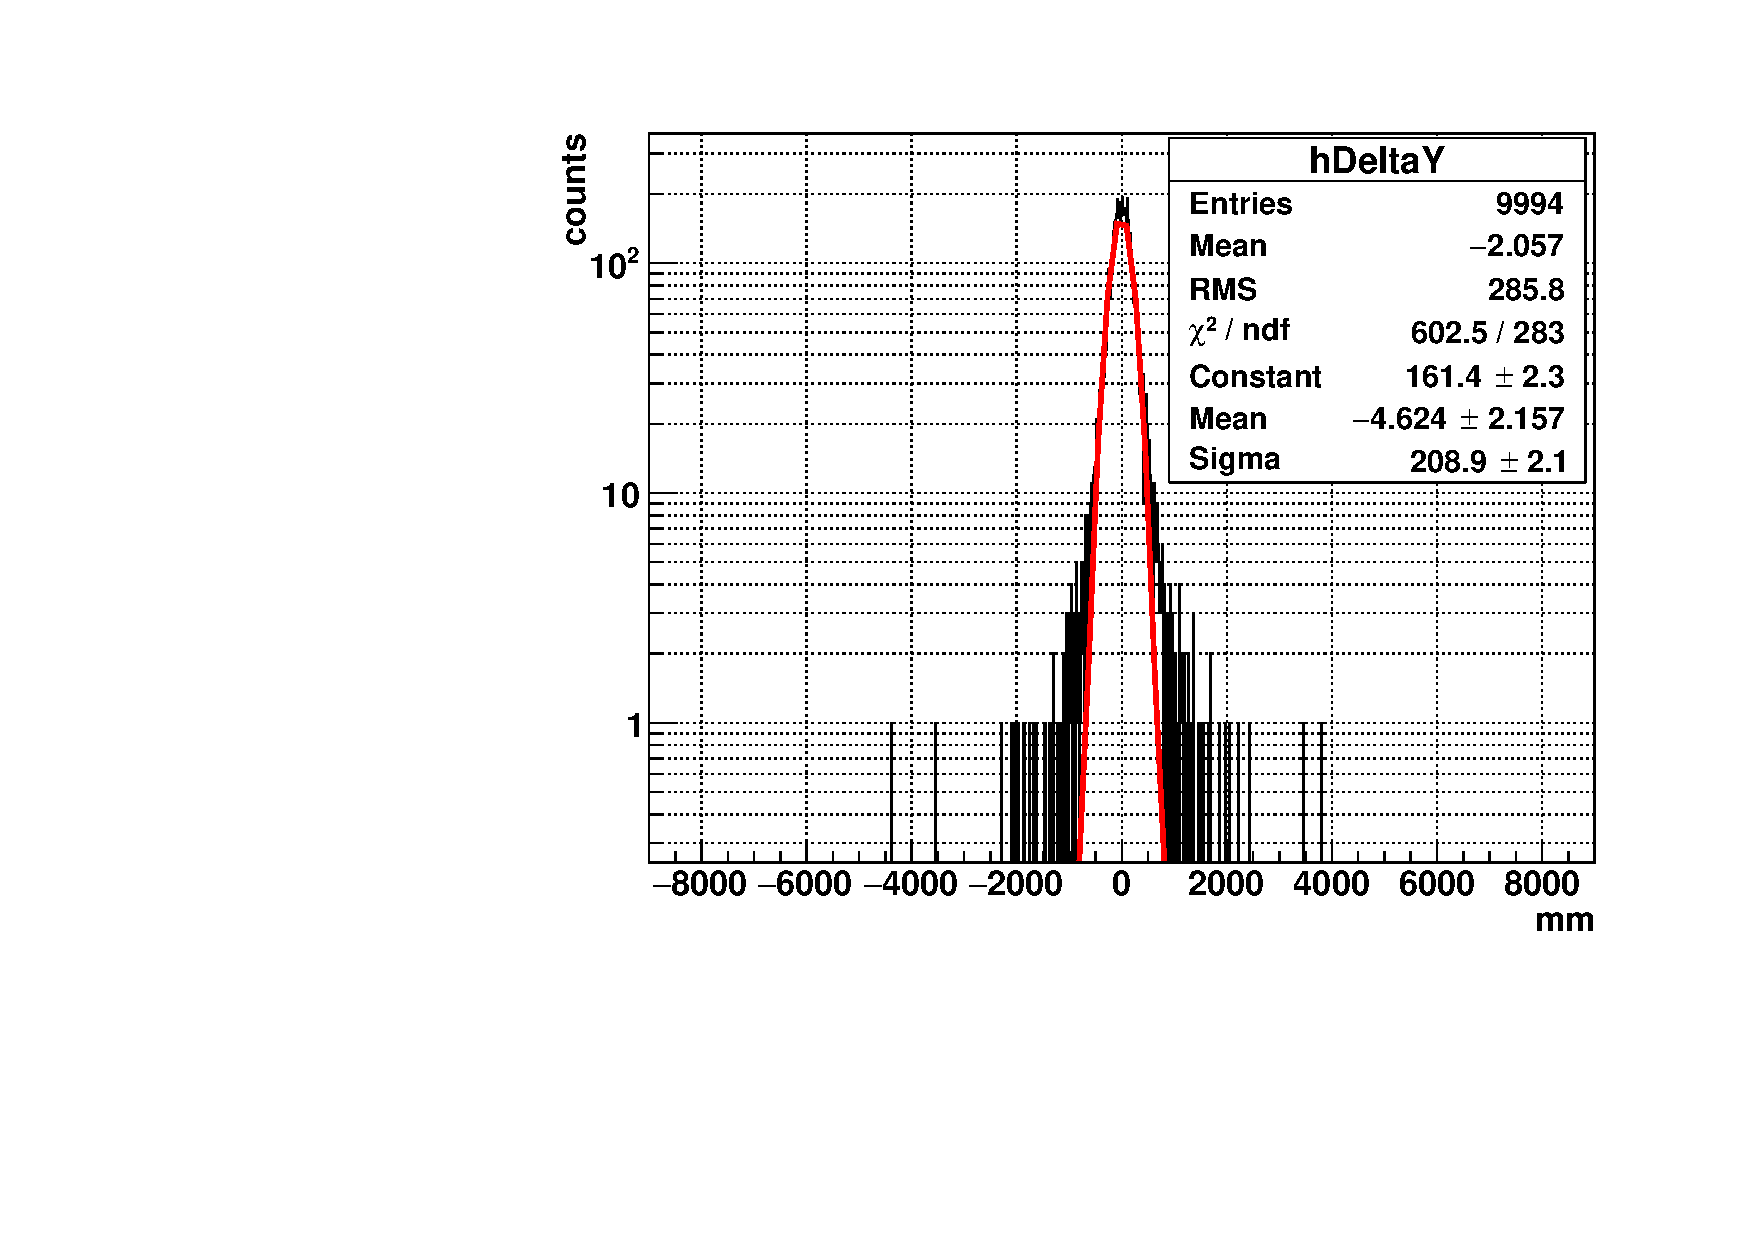
\includegraphics[width=8cm]{5MeVbetaY.pdf}
		\end{minipage}
	}
	\subfigure[$z_{fit}-z_{mc}$]{ 
		\begin{minipage}[b]{0.4\textwidth}
			\centering
			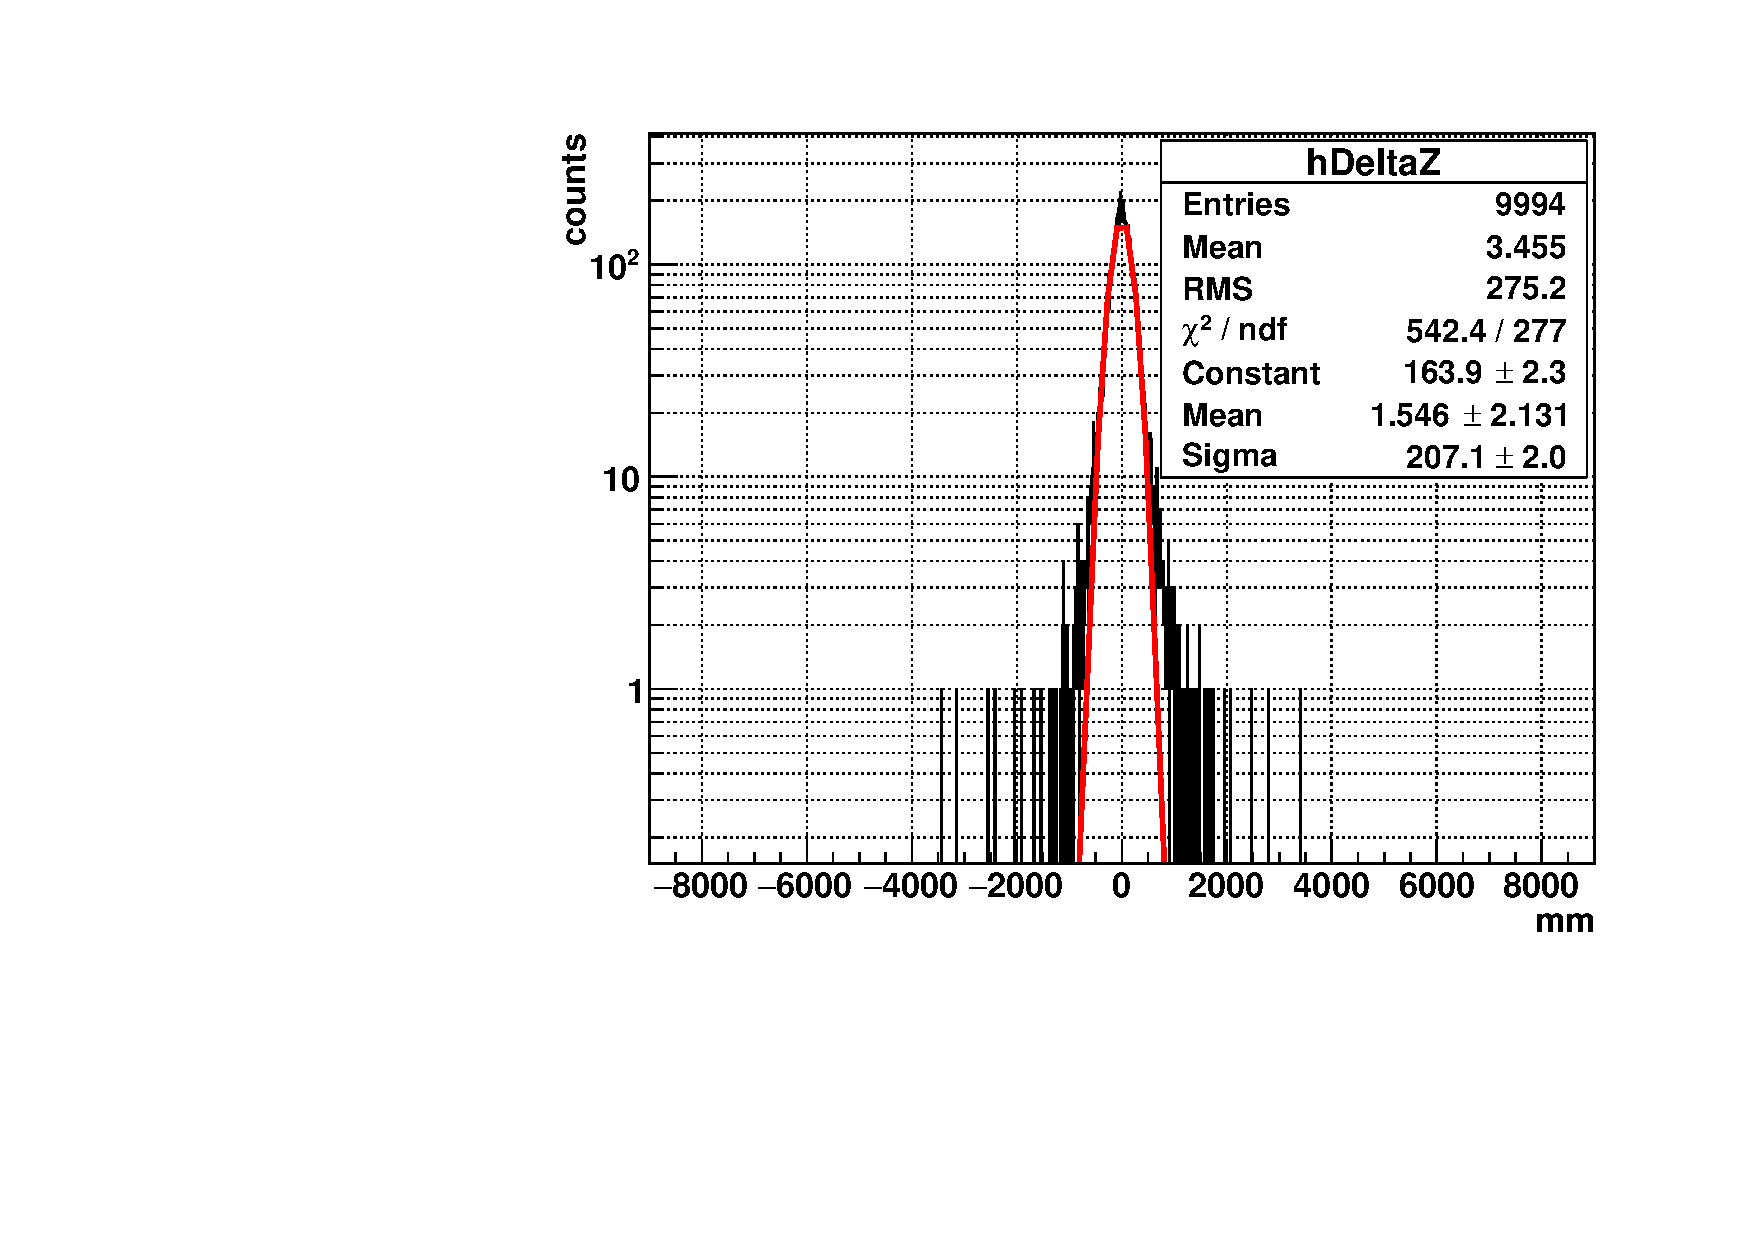
\includegraphics[width=8cm]{5MeVbetaZ.pdf}
		\end{minipage}
	}
	\caption[The position biases projected on the x, y and z axes.]{The position biases projected on the x, y and z axes. The distributions were fitted with Gaussian functions. The MC generated 10000 5-MeV $e^-$ particles at the detector center with isotropic directions.}
\end{figure}

In Fig.~\ref{fig:5MeVbeta_center_water}, there are a few events with position biases larger than 2000 mm, which are considered as mis-reconstruct events. Some of these events are due to relatively lower log-likelihood values and can be tagged by the $posFoM$ mentioned in Sect.~\ref{sect:positinFoM}. As shown in Fig.~\ref{fig:posFOM_5MeVbeta_center_water}, a cut of $scaleLogL>10$ can remove a few mis-reconstructed events. The rest of them can be caused by the straight light path calculation in the \texttt{MP fitter}, since this calculation omits the complicated situations with the refraction and reflection light paths, as mentioned in Sect.~\ref{sect:waterVertex}. However, the fraction of these mis-reconstruct events is low, about 0.1\% and thus it is acceptable.

\begin{figure}[htbp]
	\centering \label{fig:posFOM_5MeVbeta_center_water}
	\subfigure[$x_{fit}-x_{mc}$ vs. $scaleLogL$.]{
		\begin{minipage}[t]{0.5\textwidth}
			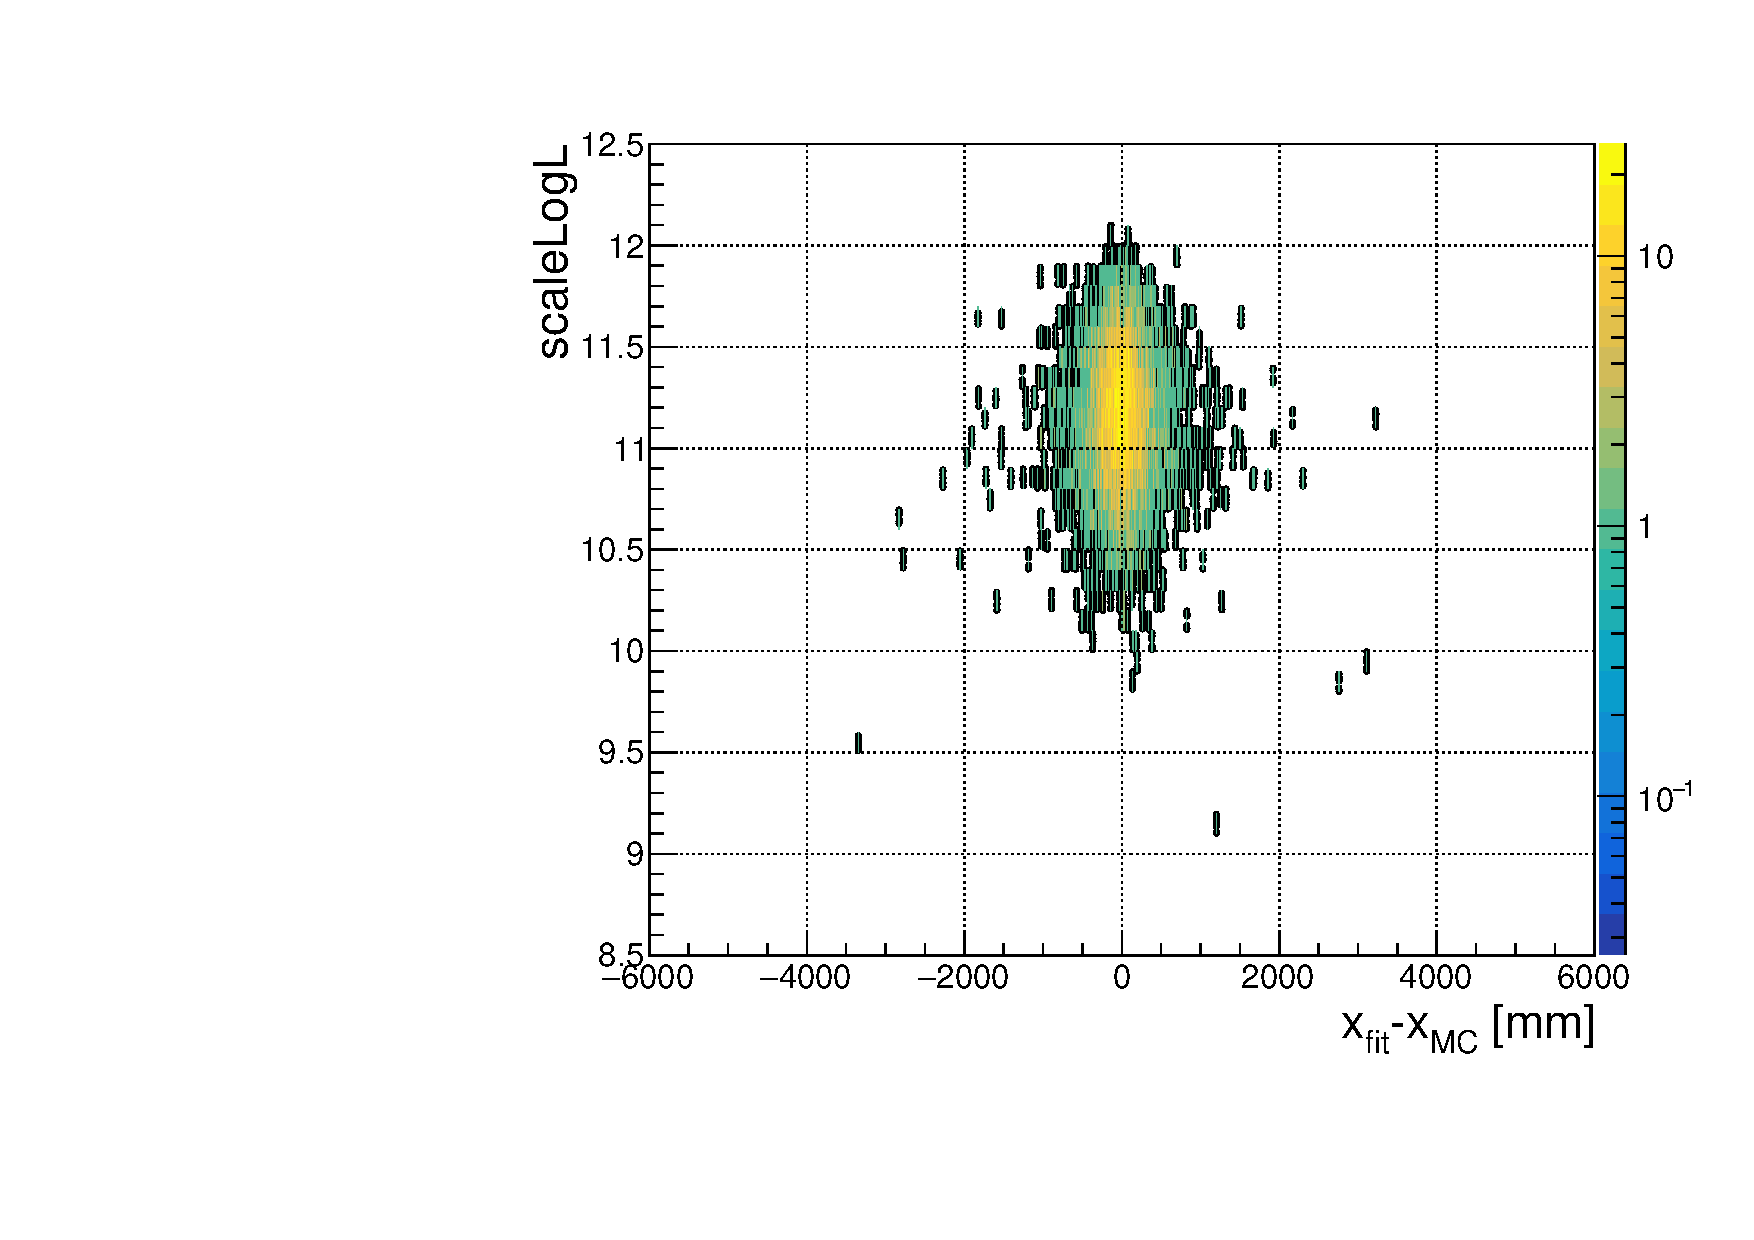
\includegraphics[width=8cm]{scaleLogLvsX_water5MeV.pdf}
		\end{minipage}
	}   
	\subfigure[$y_{fit}-y_{mc}$ vs. $scaleLogL$.]{ 
		\begin{minipage}[t]{0.4\textwidth}
			\centering
			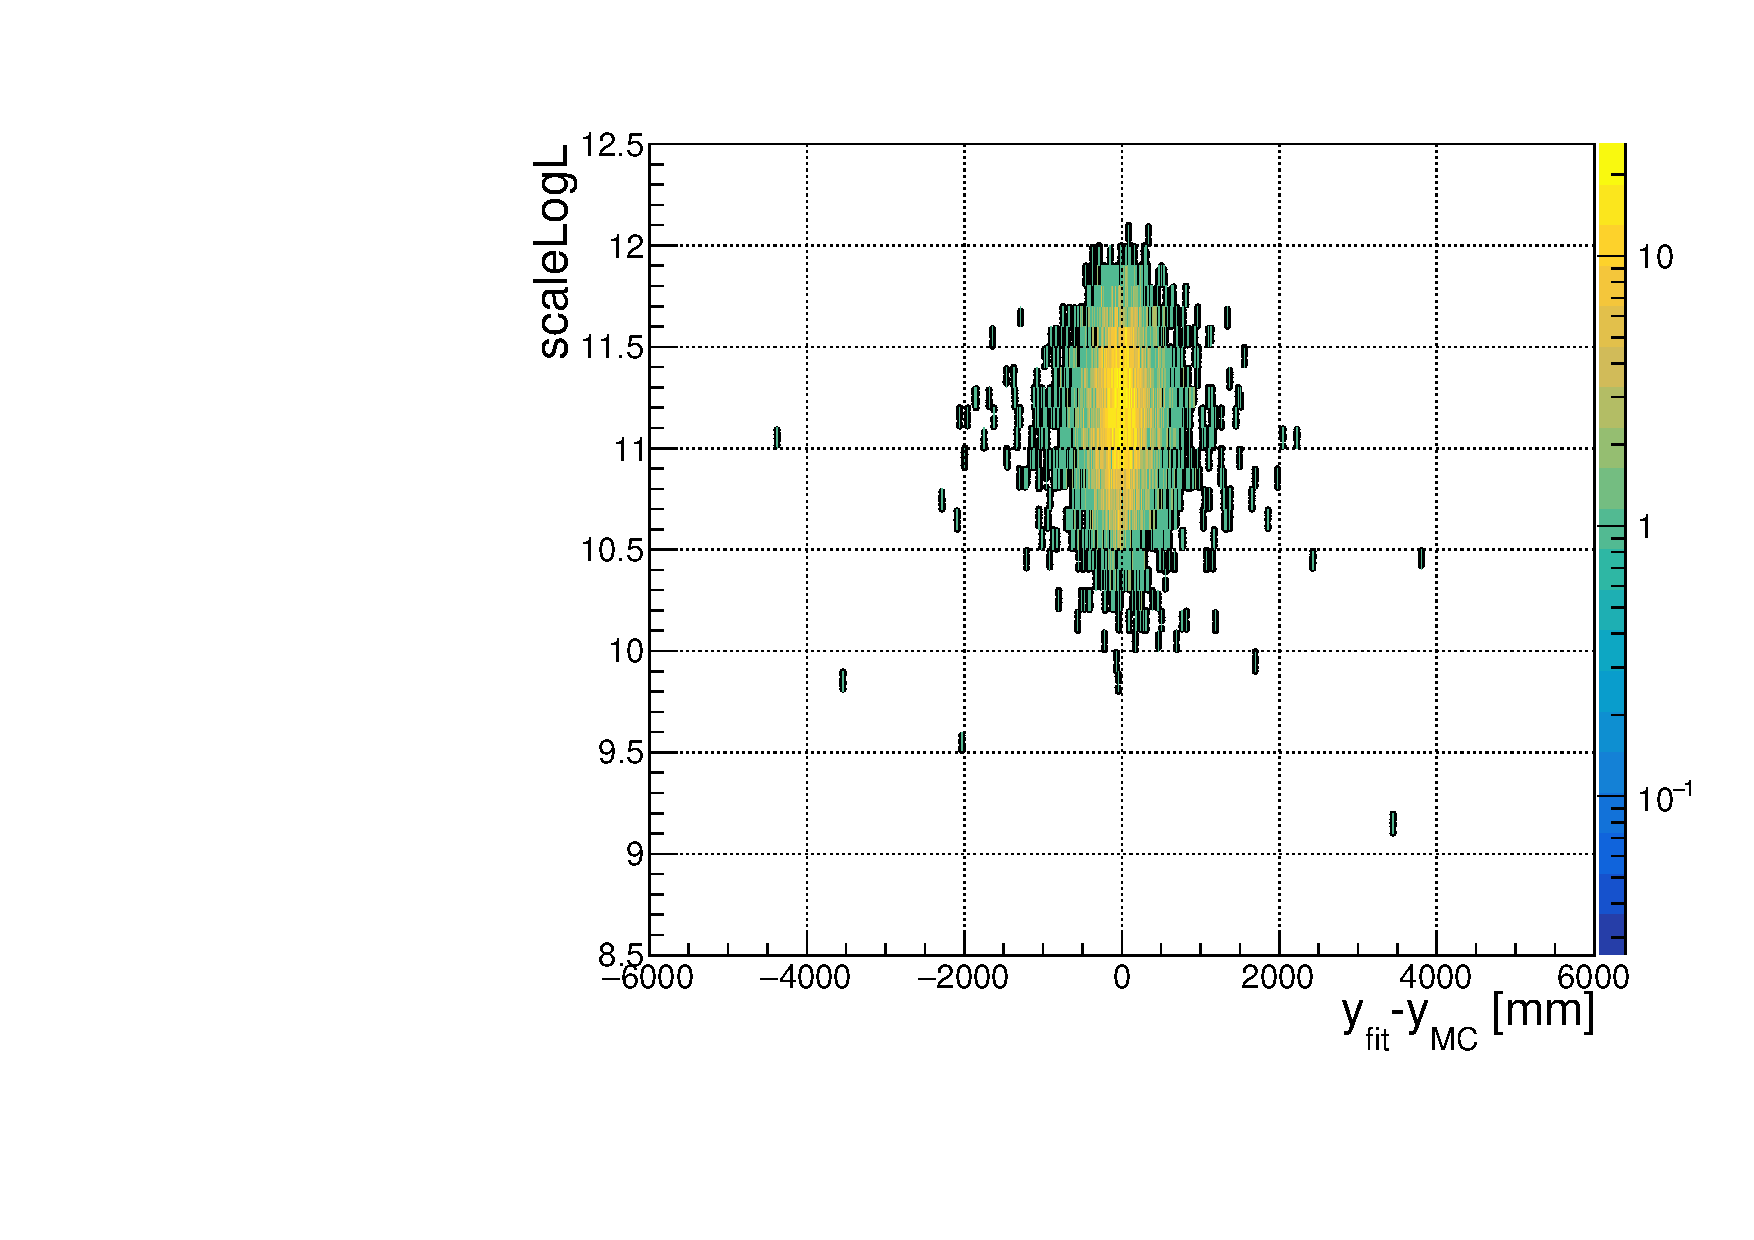
\includegraphics[width=8cm]{scaleLogLvsY_water5MeV.pdf}
		\end{minipage}
	}
	\subfigure[$z_{fit}-z_{mc}$ vs. $scaleLogL$.]{ 
		\begin{minipage}[b]{0.4\textwidth}
			\centering
			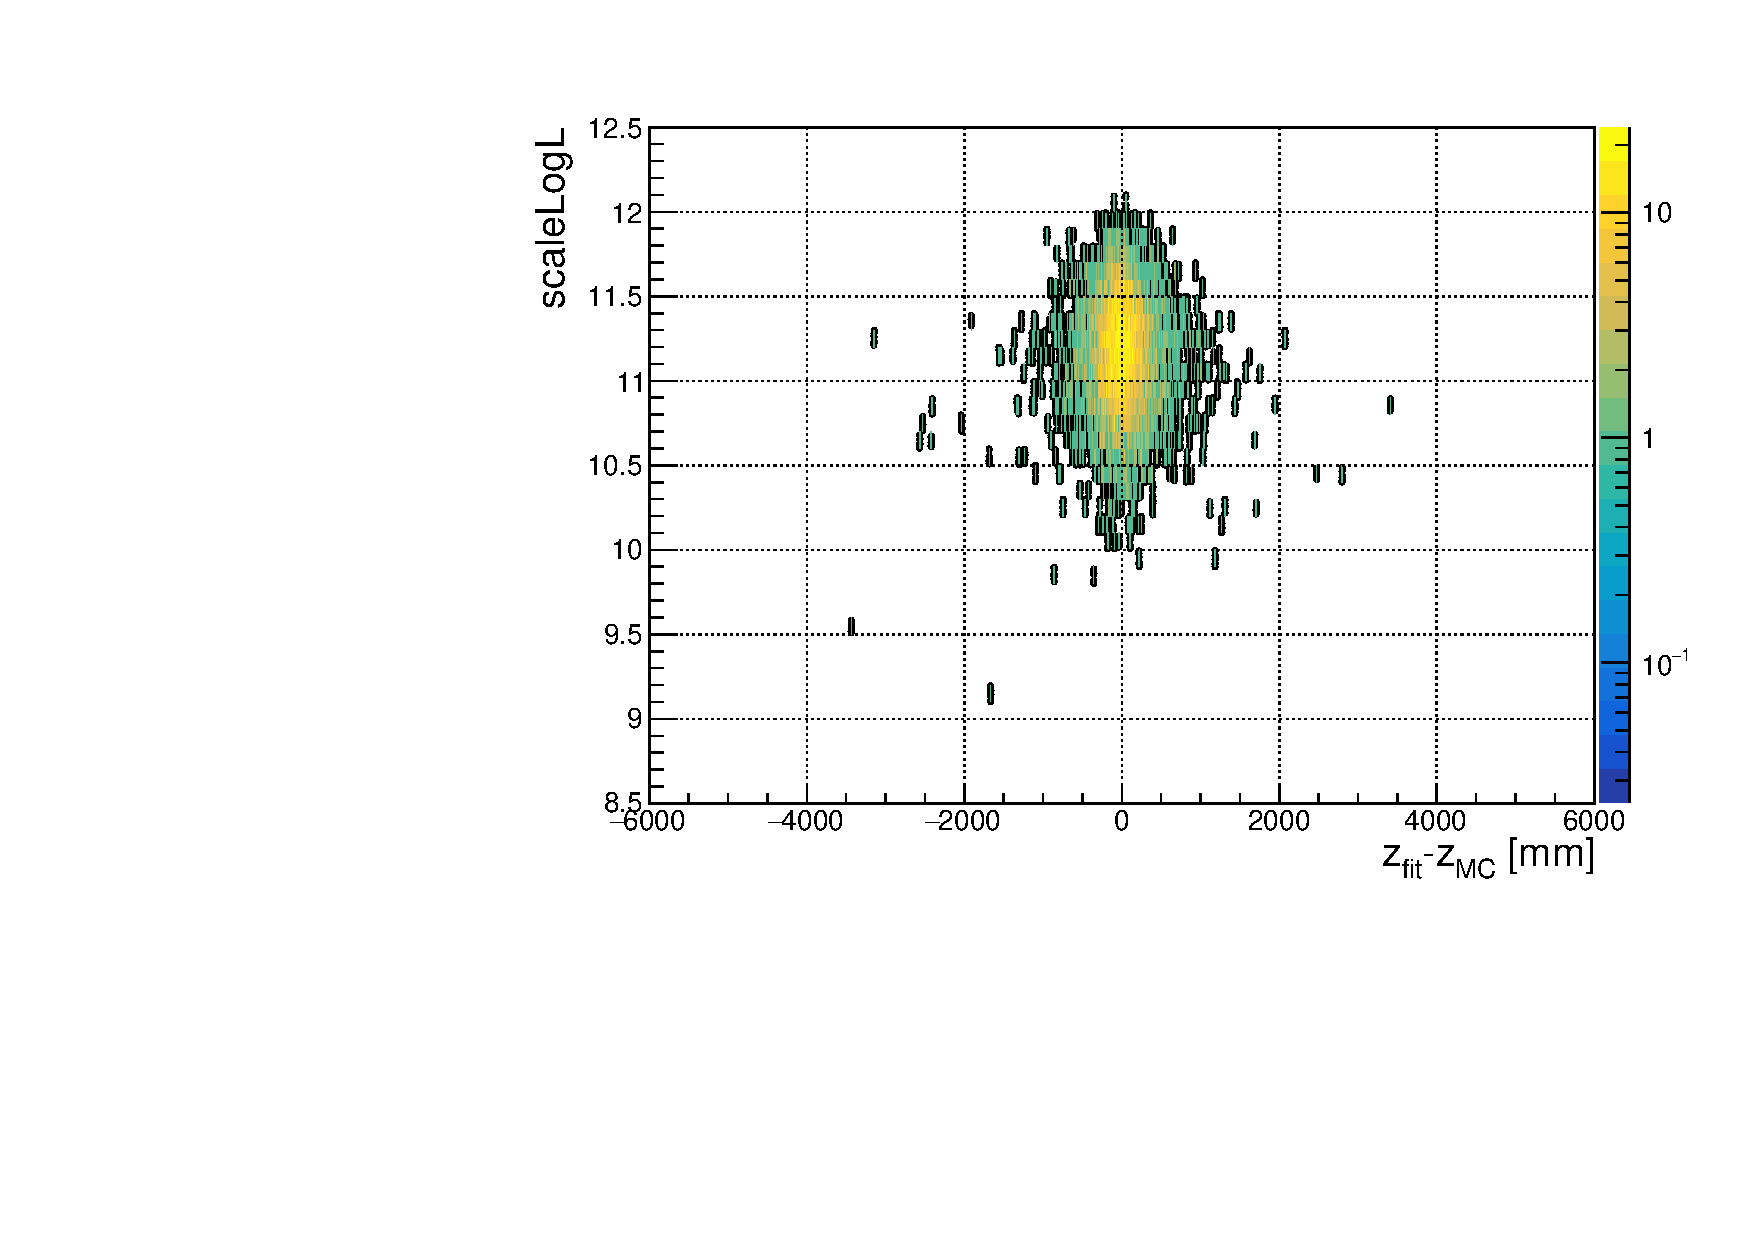
\includegraphics[width=8cm]{scaleLogLvsZ_water5MeV.pdf}
		\end{minipage}
	}
	\caption[The position biases against the position FOMs.]{The position biases against the position FoMs. The MC generated 10000 5-MeV $e^-$ particles at the detector center with isotropic directions.}
\end{figure}

A more generic situation is that the events happen everywhere inside the AV. To simulate this, $e^-$ events were generated at random positions uniformly distributed inside the AV volume and with isotropic directions. Various $e^-$ energies were also simulated, from 2 to 15 MeV with a 1-MeV step. Fig.~\ref{fig:MPWposBias_isoFill} and Fig.~\ref{fig:MPWposResol_isoFill} show the fit position biases ($\mu_{x,y,z}$) and resolutions ($\sigma_{x,y,z}$) respectively. 

These results show that the fit position biases $\mu_{x,y,z}$ are stable across different energies and for $E\leq 5$ MeV, the biases are within 10 mm.
The resolutions $\sigma_{x,y,z}$ decrease from about 350 mm to 120 mm and the average is 180 mm. More photons are produced by the $e^-$ events with higher energy, thus triggering more PMTs. With a larger NHits value, more information is provided for the fitter, and it can return better position resolutions. As I will show in the following section, the position resolution can also be improved by using a decent detection medium that can produce more photons for the same event.. 

With a larger value of NHits, more information is provided for the fitter, and it can return better position resolutions. As I will show in the following section, the position resolution can also be improved by using a decent detection medium that can produce more photons for the same event. 

\begin{figure}[htbp]
	\centering	
	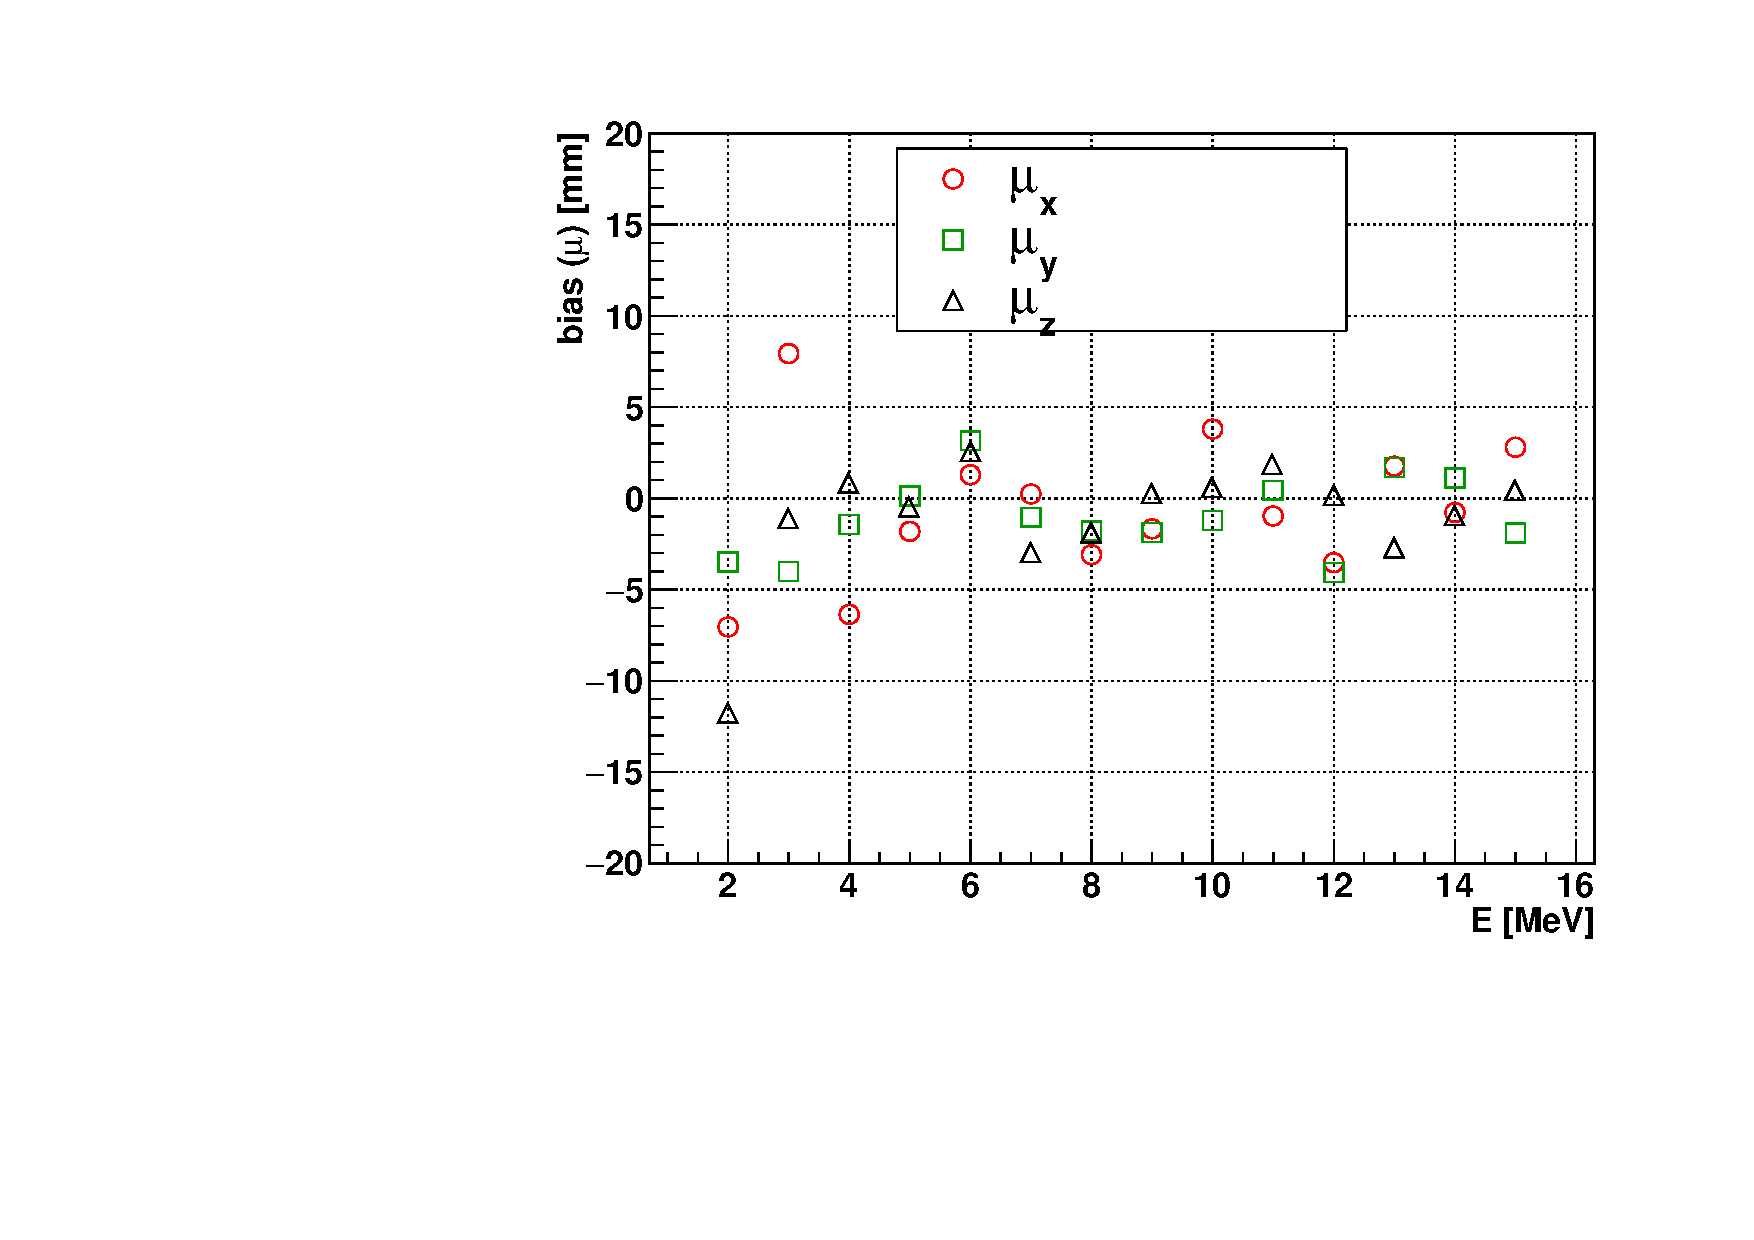
\includegraphics[width=9cm]{MPW_isoFill_posBiasVsE.pdf}
	\caption[The \texttt{MPW fitter} fit position biases ($\mu_{x,y,z}$) as a function of energy.]{The \texttt{MPW fitter} fit position biases in x(red circle), y (green square), and z (black triangle) axes as a function of energy.}
	\label{fig:MPWposBias_isoFill}
\end{figure}

\begin{figure}[htbp]
	\centering	
	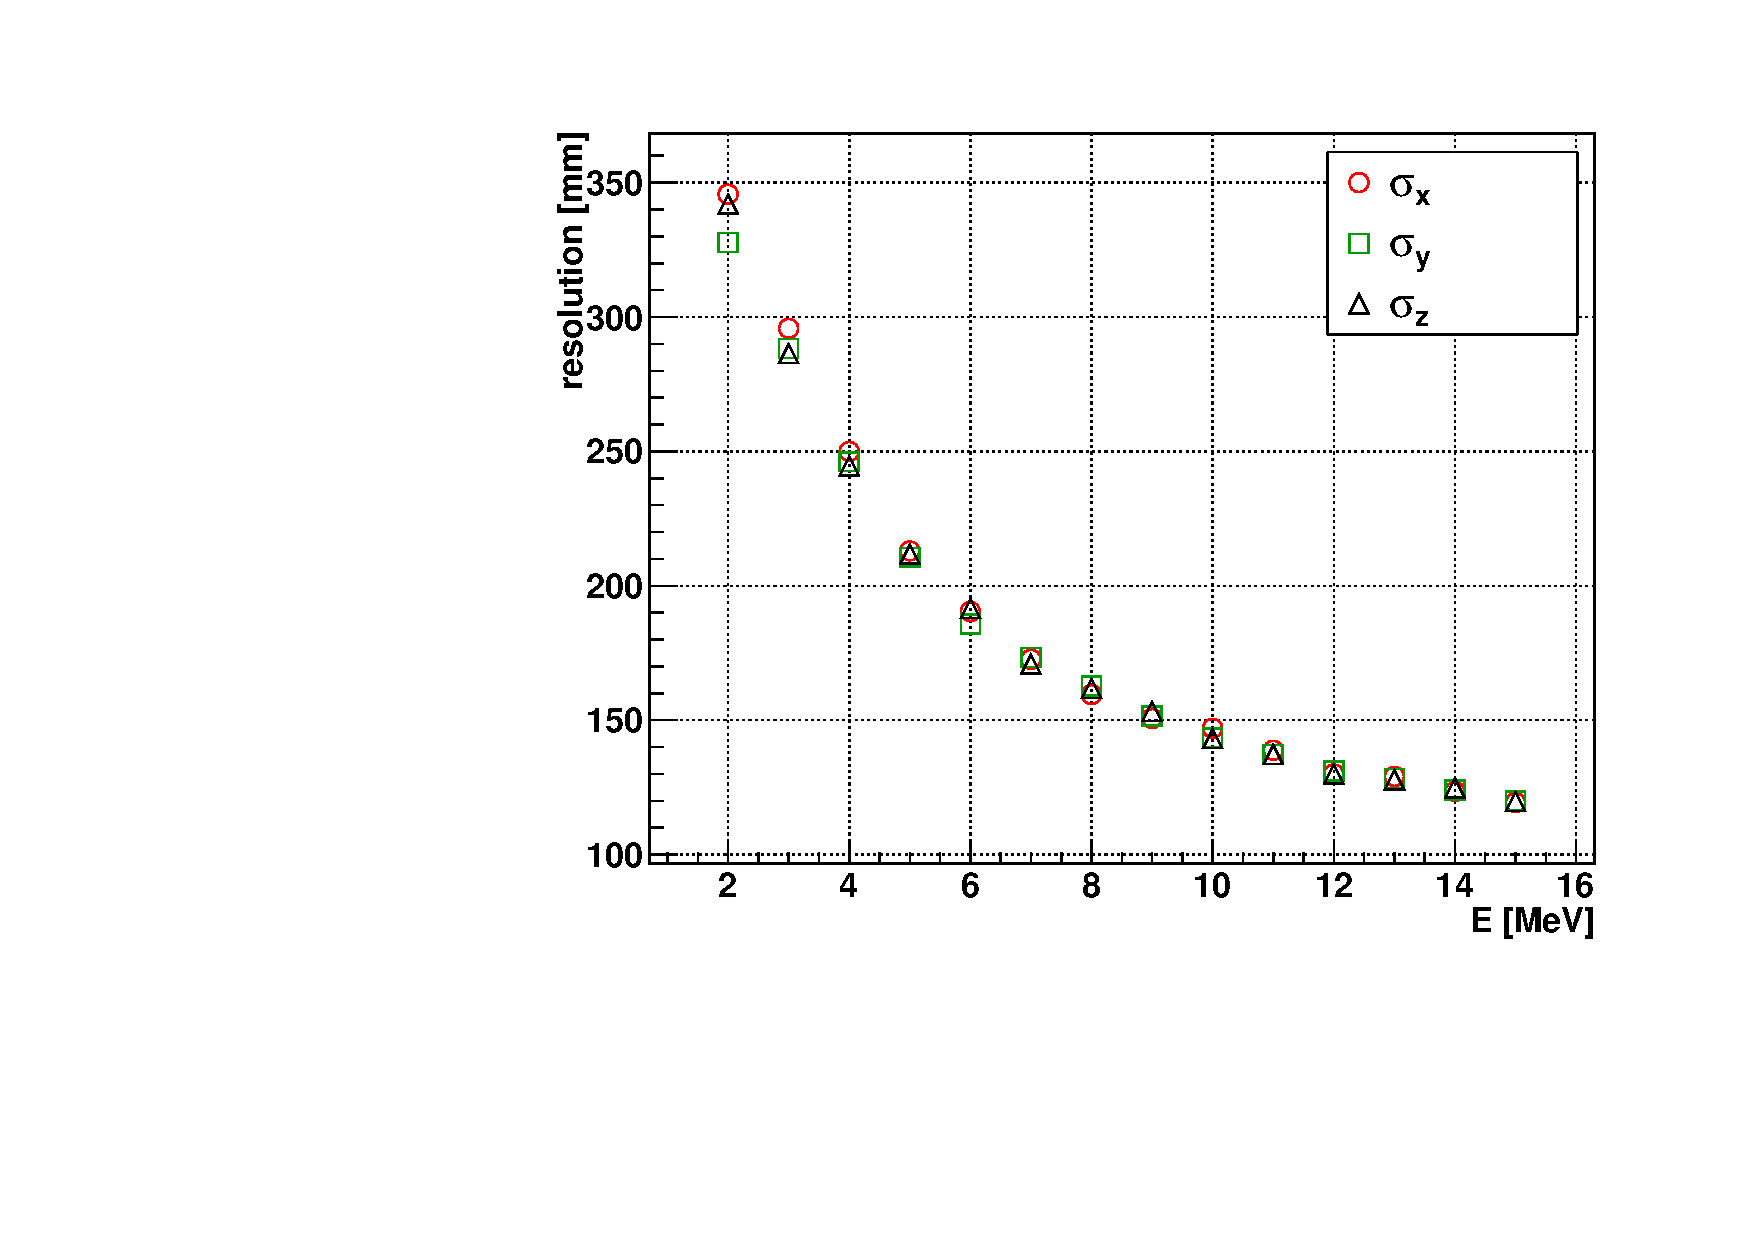
\includegraphics[width=9cm]{MPW_isoFill_posResolVsE.pdf}
	\caption[The \texttt{MPW fitter} fit position resolutions ($\sigma_{x,y,z}$) as a function of energy.]{The \texttt{MPW fitter} fit position resolutions in x (red circle), y (green square), and z (black triangle) axes as a function of energy.}
	\label{fig:MPWposResol_isoFill}
\end{figure}

To check the radial dependence of the reconstruction performance, simulations of the 5-MeV $e^-$ were generated in 11 thin shells, with isotropic directions. The centers of these shells are at the AV center, and their radii are at $r$ m and $r+0.001$ m, where $r$ is from 0.5 m to 5.5 m, with a step of 0.5 m. Fig.~\ref{fig:FitBiasVsShell} and Fig.~\ref{fig:FitResolVsShell} show the fit position biases and resolutions respectively. The results show that the fit position biases are stable across the different radii of the AV, while the resolutions become worse when the events are close to the AV, or $R>5$ m. This is called the ``near AV effect'', which was observed in SNO. For the position close to the AV, the AV can serve as a lens and distort the light path\cite{brice1996monte}. A few complicated calculations to tackle this effect and the technique called ``Near AV cut'' were discussed in Refs.~\cite{coulter2013modelling,jones2011background}, but they are not applied in this thesis. 

\begin{figure}[htbp]
	\centering	
	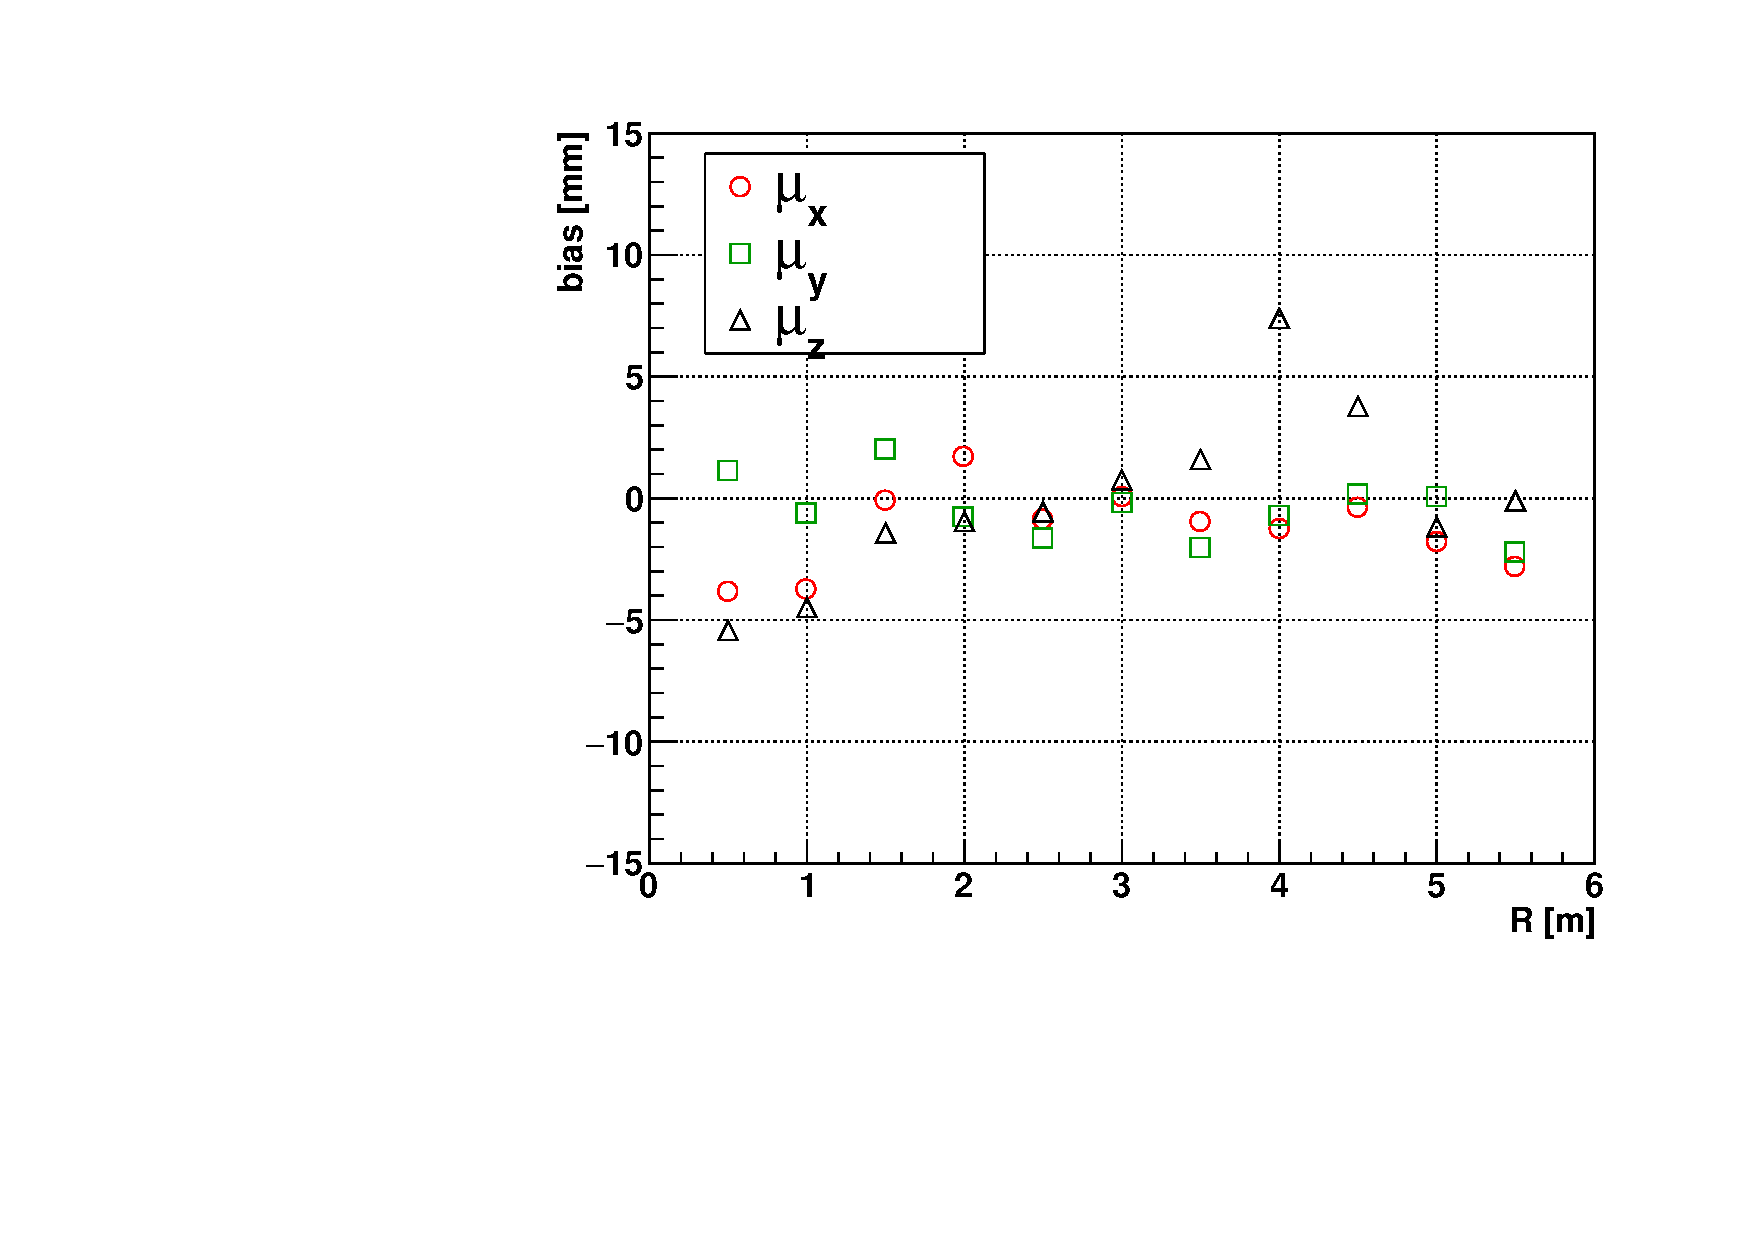
\includegraphics[width=9cm]{shellTest_RvsBias.pdf}
	\caption[The \texttt{MPW fitter} fit position biases ($\mu_{x,y,z}$) as a function of energies.]{The \texttt{MPW fitter} fit position biases of x (red circle), y (green square), and z (black triangle) axes as a function of radius.}
	\label{fig:FitBiasVsShell}
\end{figure}

\begin{figure}[htbp]
	\centering	
	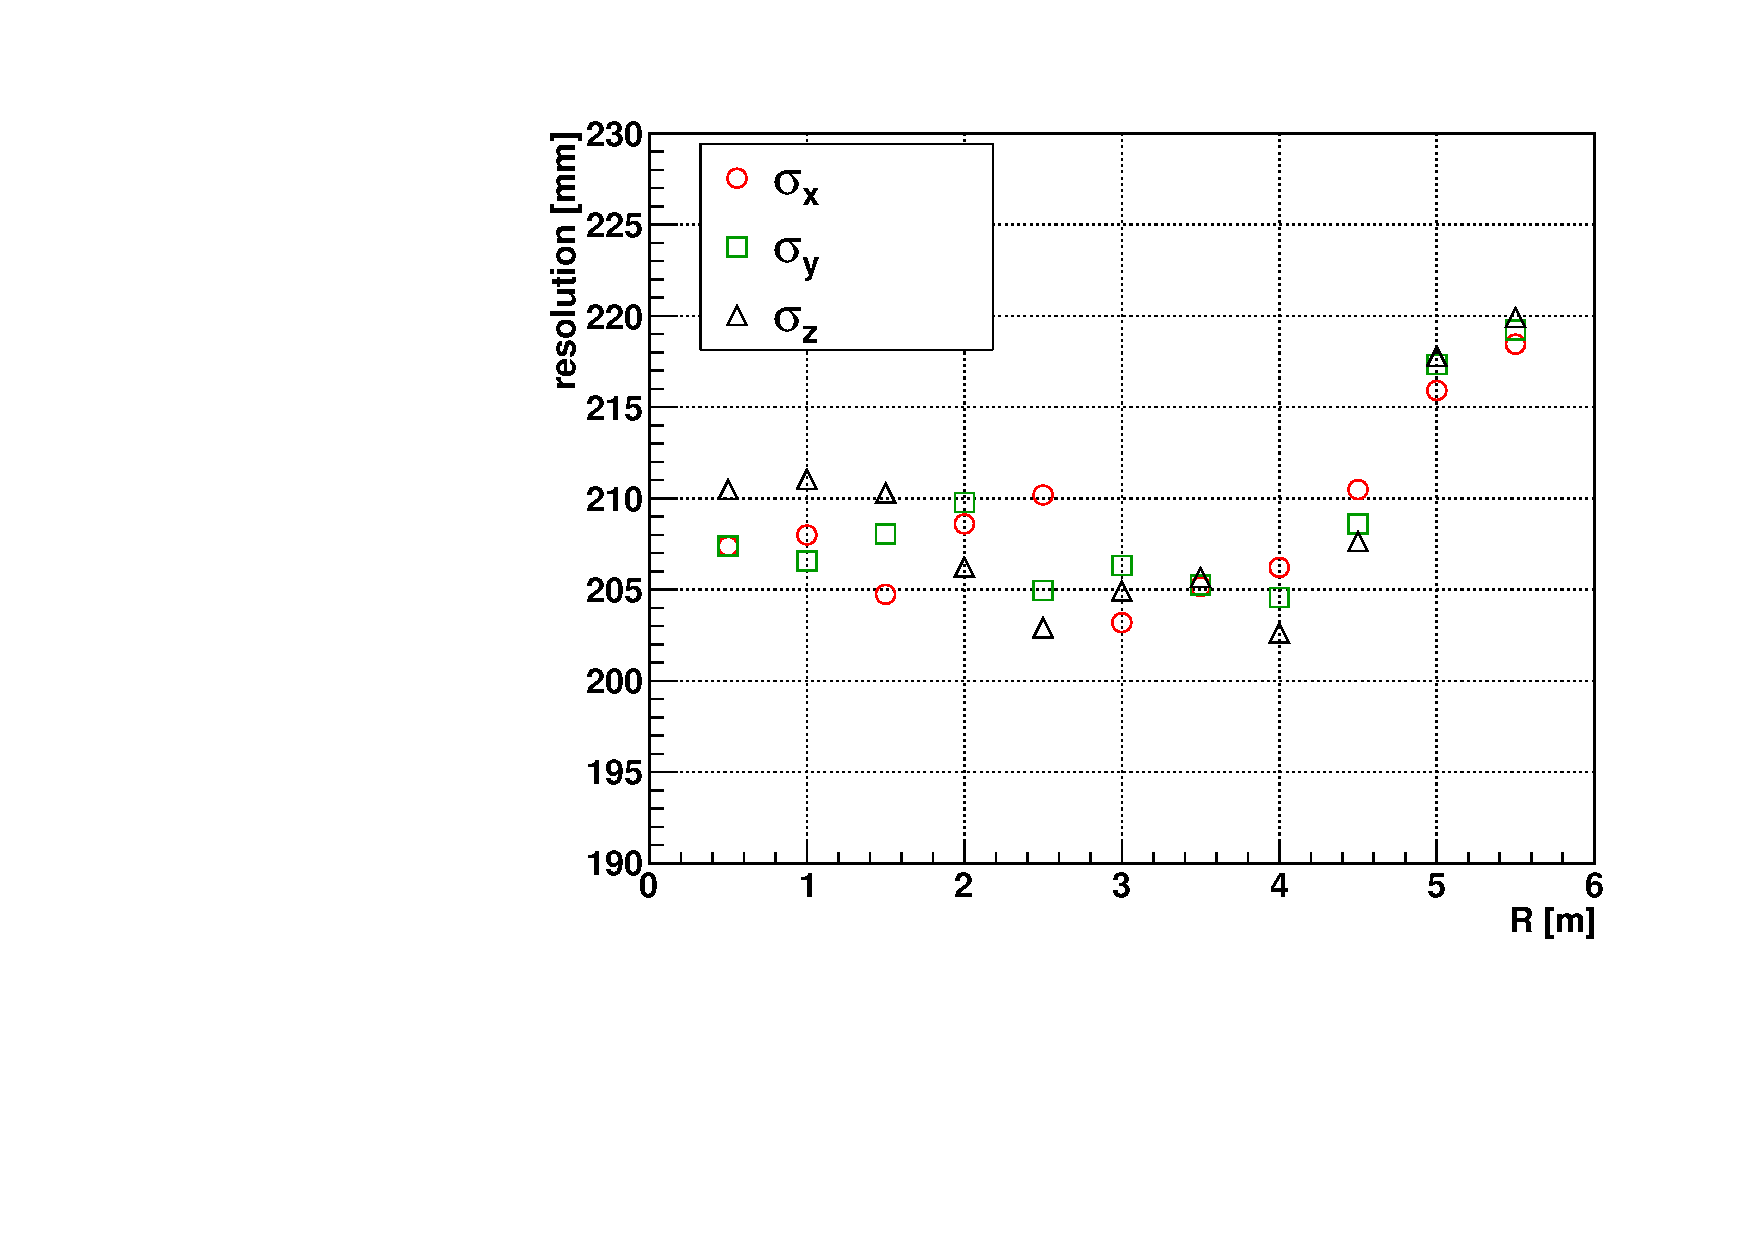
\includegraphics[width=9cm]{shellTest_RvsResol.pdf}
	\caption[The \texttt{MPW fitter} position resolutions ($\sigma_{x,y,z}$) as a function of energies.]{The \texttt{MPW fitter} position resolutions of x (red circle), y (green square), and z (black triangle) axes as a function of radius.}
	\label{fig:FitResolVsShell}
\end{figure}
 
\subsection{Performances of the Water Direction Reconstruction}\label{sect:directResol}
The bias between the true event direction $\vec{u}_{MC}$ and the reconstructed direction $\vec{u}_{fit}$ is described by the angle $\theta_e$, and $\cos\theta_e\equiv\vec{u}_{fit}\cdot\vec{u}_{MC}$.

To describe the distribution of $\cos\theta_e$, an empirical function for the angular resolution was adopted by SNO\cite{boulay2004direct} and it is defined as a combination of two exponential components:
\begin{equation}\label{eq:directResol}
P(\cos\theta_e)=\alpha_M\frac{\beta_M\exp[-\beta_M(1-\cos\theta_e)]}{1-\exp(-2\beta_M)}+(1-\alpha_M)\frac{\beta_s\exp[-\beta_s(1-\cos\theta_e)]}{1-\exp(-2\beta_s)},
\end{equation}
where the parameters: $\beta_M$ and $\beta_S$ are the ``decay'' constants or the ``slopes'' of the two exponential components; $\alpha_M$ is the fraction between two exponential components. The first component, the main peak is due to the single scattering of the electrons and is the true angular resolution of the detector, while the second component which has a broad tail is mainly due to the multiple scattering of electrons; there are also back scattering electrons on the detector components and the poorly reconstructed events in the tails\cite{boulay2004direct}. Fig.~\ref{fig:directionResol_5MeV} shows the $\cos\theta_e$ distribution of the 5-MeV $e^-$ particles generated at the detector center and with isotropic directions.

\begin{figure}[htbp]\label{fig:directionResol_5MeV}
	\centering
	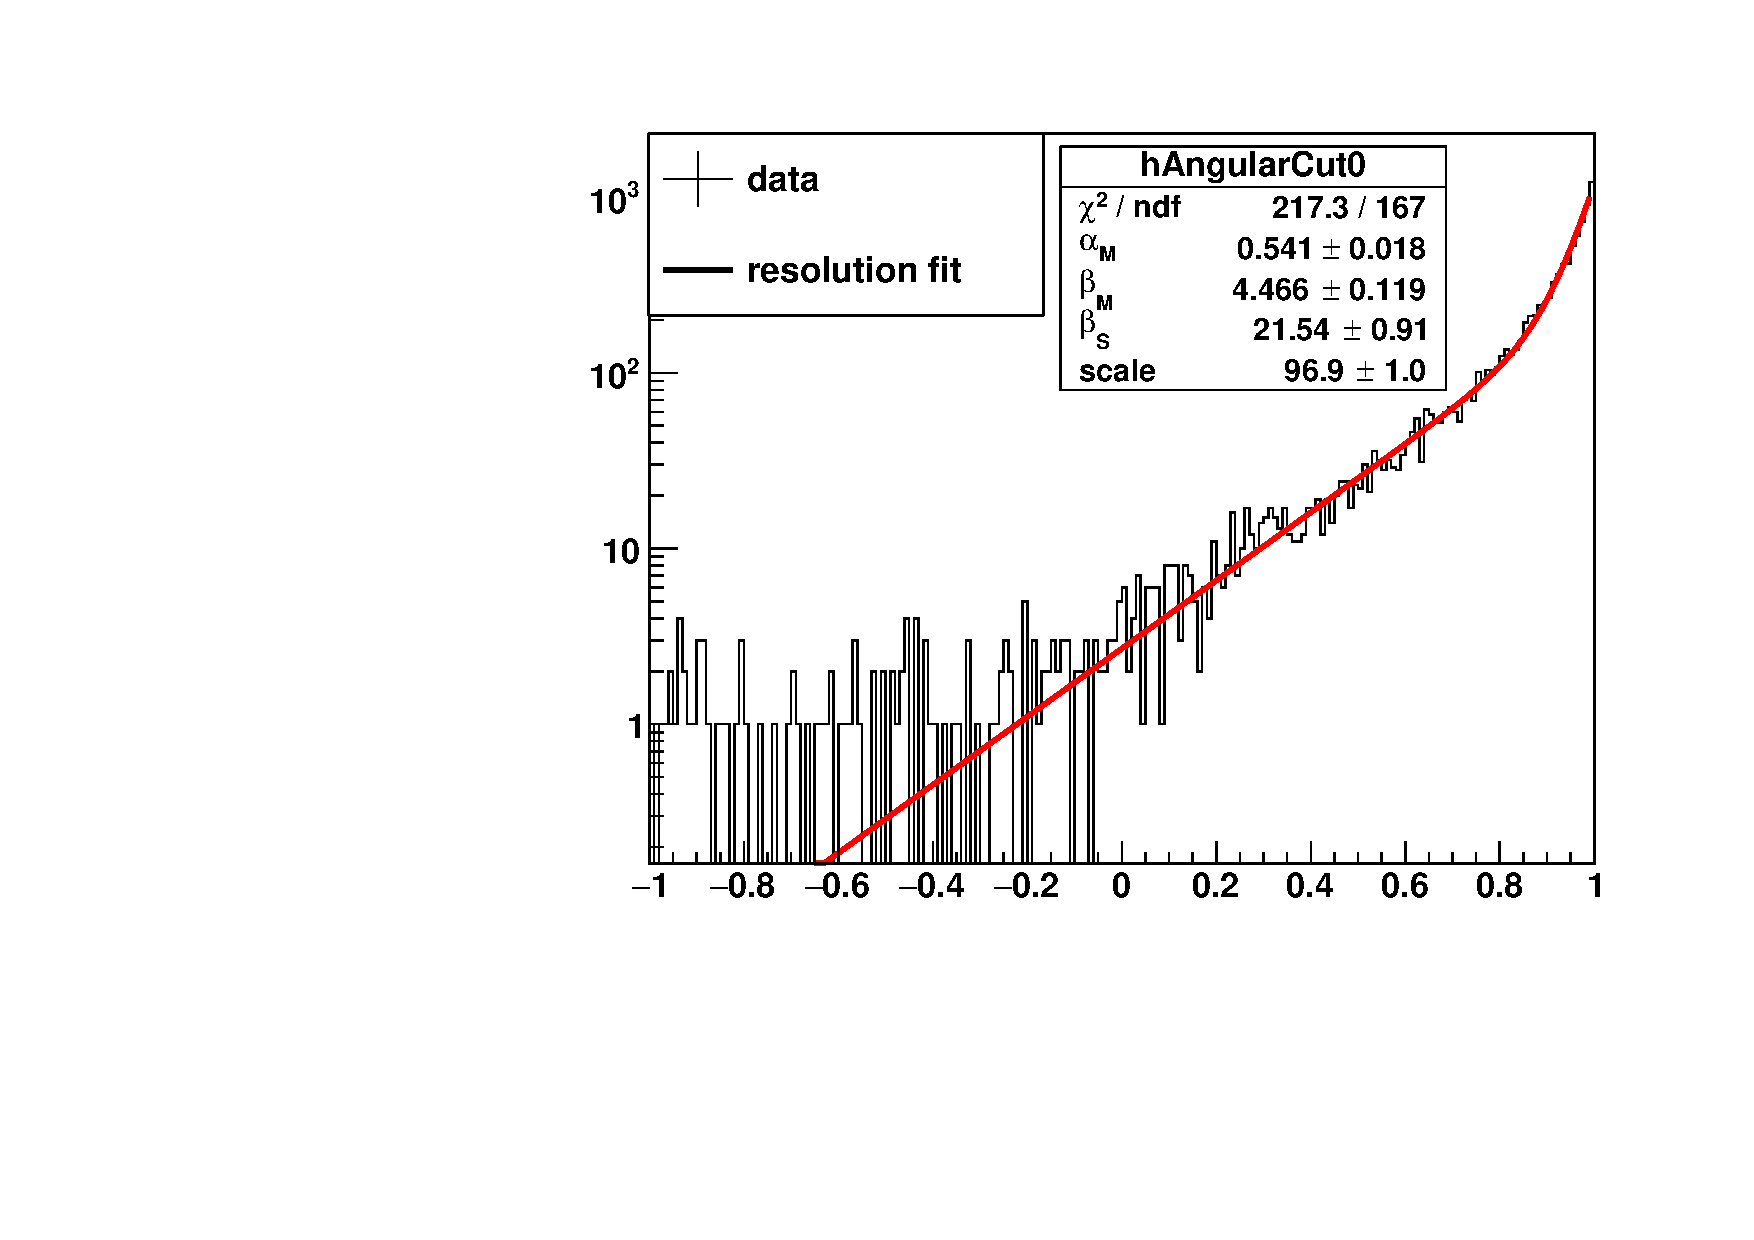
\includegraphics[width=8cm]{MPW_waterDirection_5MeV.pdf}
	\caption[The biases between the fitted and MC directions.]{The biases between the fitted and MC directions, fitted with the resolution function $P(\cos\theta_e)$ (plotted in red). The MC generated $10^4$ 5-MeV $e^-$ at the detector center.}
\end{figure}

Another way to quantify the reconstruction performance based on the $\cos\theta_e$ distribution is to calculate the angles that contain 50\%, 80\%
or 90\% of the reconstructed events, denoted by $\cos\theta_{0.5}$, $\cos\theta_{0.8}$ and $\cos\theta_{0.9}$ respectively\cite{coulter2013modelling}. Their values are solved numerically from the Eqn.~\ref{eq:cosTheta_fraction}:
\begin{equation}\label{eq:cosTheta_fraction}
\frac{\int_{\cos\theta_{a}}^1 P(\cos\theta_e) d\cos\theta_e}{\int_{-1}^1 P(\cos\theta_e) d\cos\theta_e} = a\times 100\%,
\end{equation}
where $P(\cos\theta_e)$ is the direction resolution function with the best fitted parameters. A larger $\cos\theta_{a}$ means the $\cos\theta_e$ distribution is more peaked around +1 and a better direction reconstruction. The results of the direction resolutions are listed in Table.~\ref{tab:angularResol_MPW}.

\begin{table}[ht]
	\caption{Direction resolutions for the reconstruction of the 5-MeV $e^-$ events.\label{tab:angularResol_MPW}}
	\vspace{2mm}
	\centering		
	\begin{tabular*}{110mm}{c@{\extracolsep{\fill}}cccccc}
		\toprule 
	    $\beta_M$ &  $\beta_S$ & $\cos\theta_{0.5}$ & $\cos\theta_{0.8}$& $\cos\theta_{0.9}$\\
        \hline
         4.47$\pm$0.12 & 21.54 $\pm$0.91 & 0.978 & 0.777 & 0.624\\
		\bottomrule	
	\end{tabular*}
\end{table}

These results are slightly better than the SNO fitter results for the 5-MeV $e^-$ in the heavy water, with $\beta_M=3.348\pm 0.08119, \beta_S=19.3\pm 0.6929$\cite{boulay2004direct}.

To check the radial dependence of the direction reconstruction performance, the similar tests in Sect.~\ref{sect:waterFitterVertex}
Fig.~\ref{fig:diResolVsShell_5MeV} shows the direction resolutions $\beta_M$ and $\beta_S$ as a function of the radius.
\begin{figure}[htbp]
	\centering
	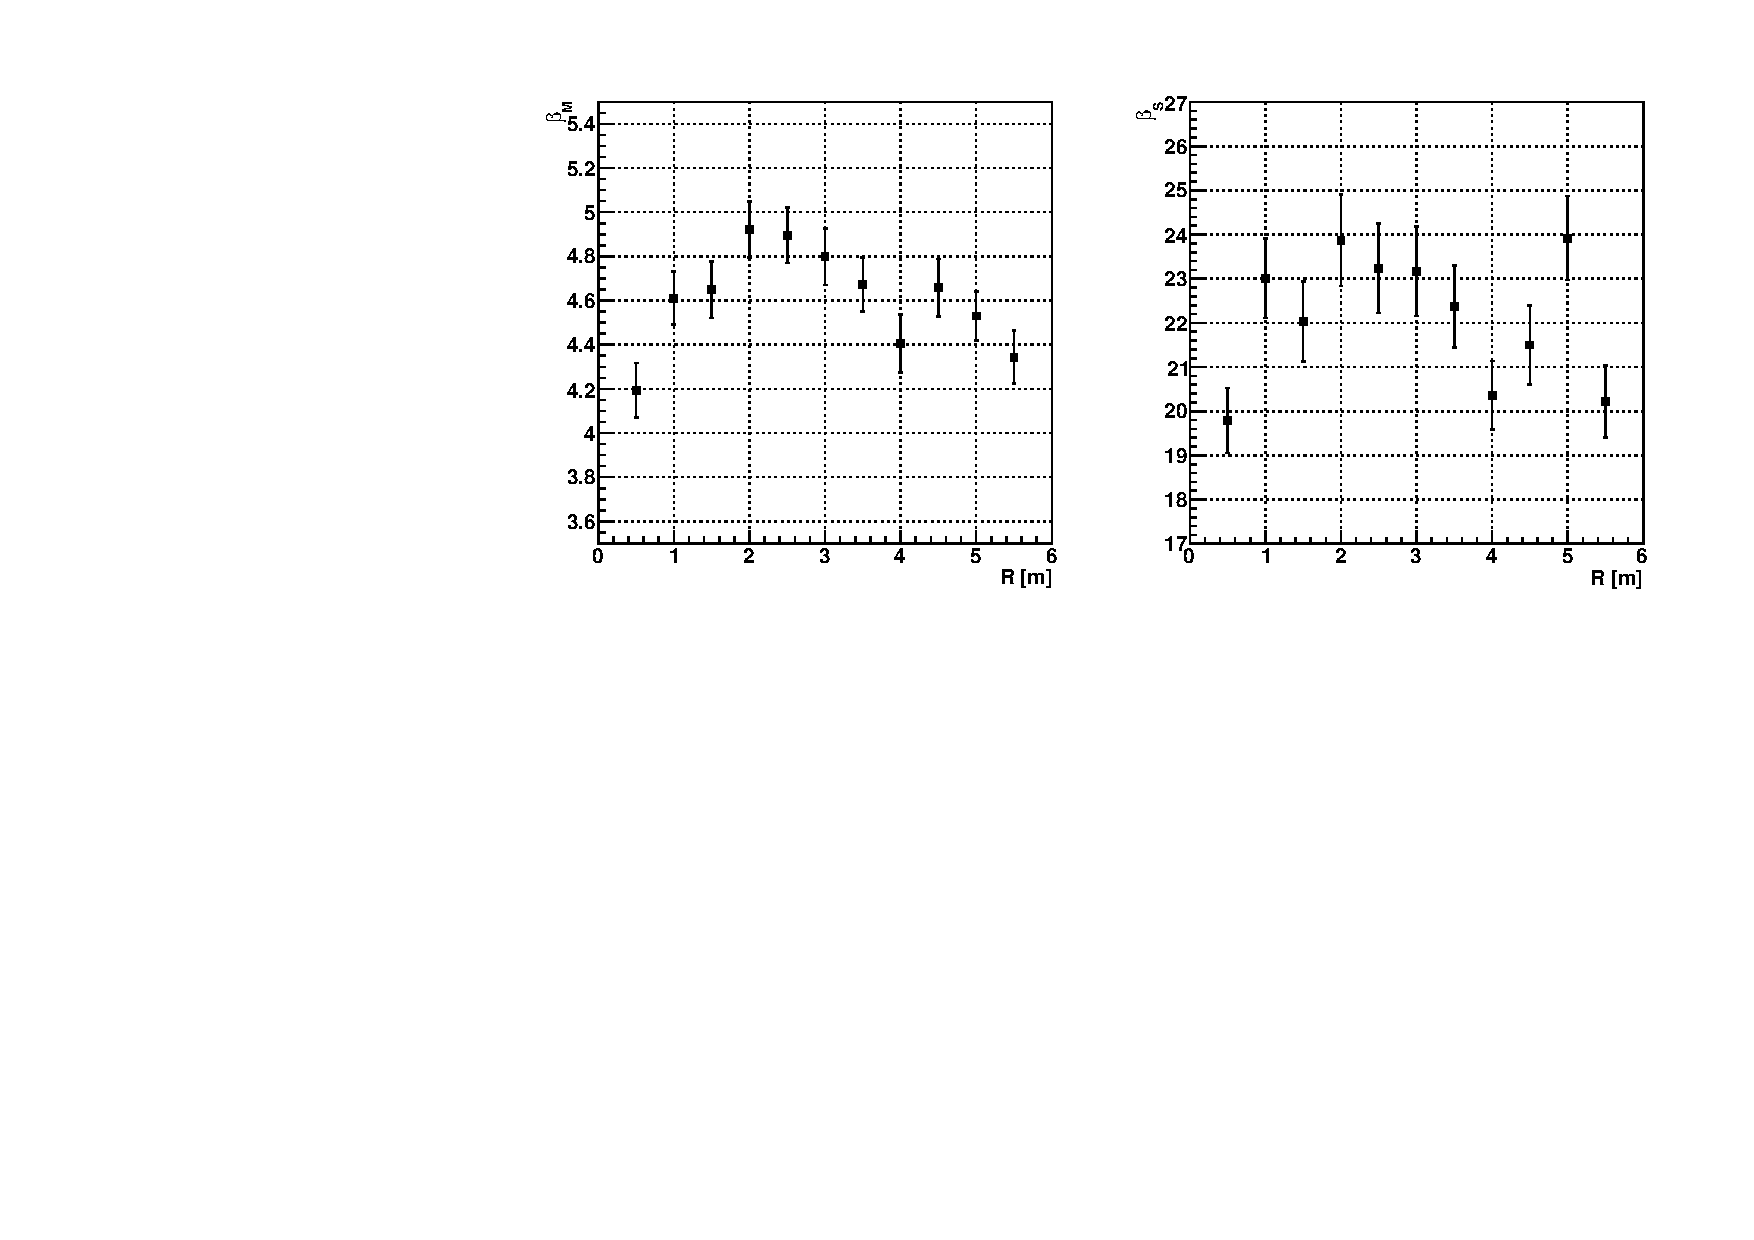
\includegraphics[width=14cm]{DirResolVsShell.pdf}
	\caption[Direction resolutions as a function of radius.]{Direction resolutions as a function of radius. The MC generated 10000 5-MeV $e^-$ inside the AV with isotropic directions.\label{fig:diResolVsShell_5MeV}}
\end{figure}

\subsection{Test on Gamma Events}

The $\gamma$ events with energies of 2.2 MeV and 4.4 MeV are crucial for analyzing the AmBe calibration data (see Sect.~\ref{sect:AmBesource}). 
A realistic trigger setting for the antineutrino analysis (run-106904) was also simulated. 
With this trigger setting in simulations, about 53\% of the low energy 2.2-MeV $\gamma$ events were triggered. So I doubled the simulations to $2\times10^4$.

Table.~\ref{tab:bias_water_gamma} shows the reconstruction performances.

\begin{table}[ht]
	\caption{Reconstruction performances for the 2.2-MeV and 4.4-MeV $\gamma$ events.}\label{tab:bias_water_gamma}
	\centering		
	\begin{tabular*}{120mm}{c@{\extracolsep{\fill}}cccc}
		\toprule 
		simulation & $\Delta x \pm \sigma_x$ [mm]& $\Delta y \pm \sigma_y$ [mm]&$\Delta z \pm \sigma_z$ [mm] \\
		\midrule
		2.2-MeV  & $2.278\pm 626.927$ & $-5.663\pm 608.182$& $-10.523\pm 626.034$\\	
		4.4-MeV  & $-6.964\pm364.725$ & $-2.804\pm 368.752$ & $-1.342\pm 368.398$\\
		\bottomrule	
	\end{tabular*}
\end{table}

\subsubsection{Test on $^{16}$N Calibration Source Events}
In a more realistic situation, the data collected from the runs of the calibration sources were used to evaluate the fitter performances as well as the reconstruction uncertainties. Chapter 5 will discuss the analyses of the $^{16}$N calibration source in detail. For these tests, a position resolution function including the distributions of the initial interaction positions, rather than the Gaussian function was used, while the same direction resolution function was used. 

\section{Vertex and Direction Reconstruction for the Water-based Wavelength-shifter}\label{sect:WLSfitter}
A reconstruction algorithm was developed to investigate the proposal for the water-based wavelength-shifter, as mentioned in \ref{sect:wbWLS}.

Figure~\ref{pmt_wls} shows the position distributions of hit PMTs for MC simulated 5 MeV electrons traveling along $+x$ direction in the AV. The left panel shows the case when the detector is filled with pure water while the right panel is for water plus 0.1 ppm PPO. For the same electrons, the number of hit PMTs (NHits) in wbWLS is about 2.4 times greater than the pure water one. Although there is extra isotropic light emitted, the Cherenkov ring can still be seen clearly, allowing reconstruction of the directionality.  

\begin{figure}[htbp]
	\centering
	\begin{minipage}[t]{0.48\textwidth}
		\centering
		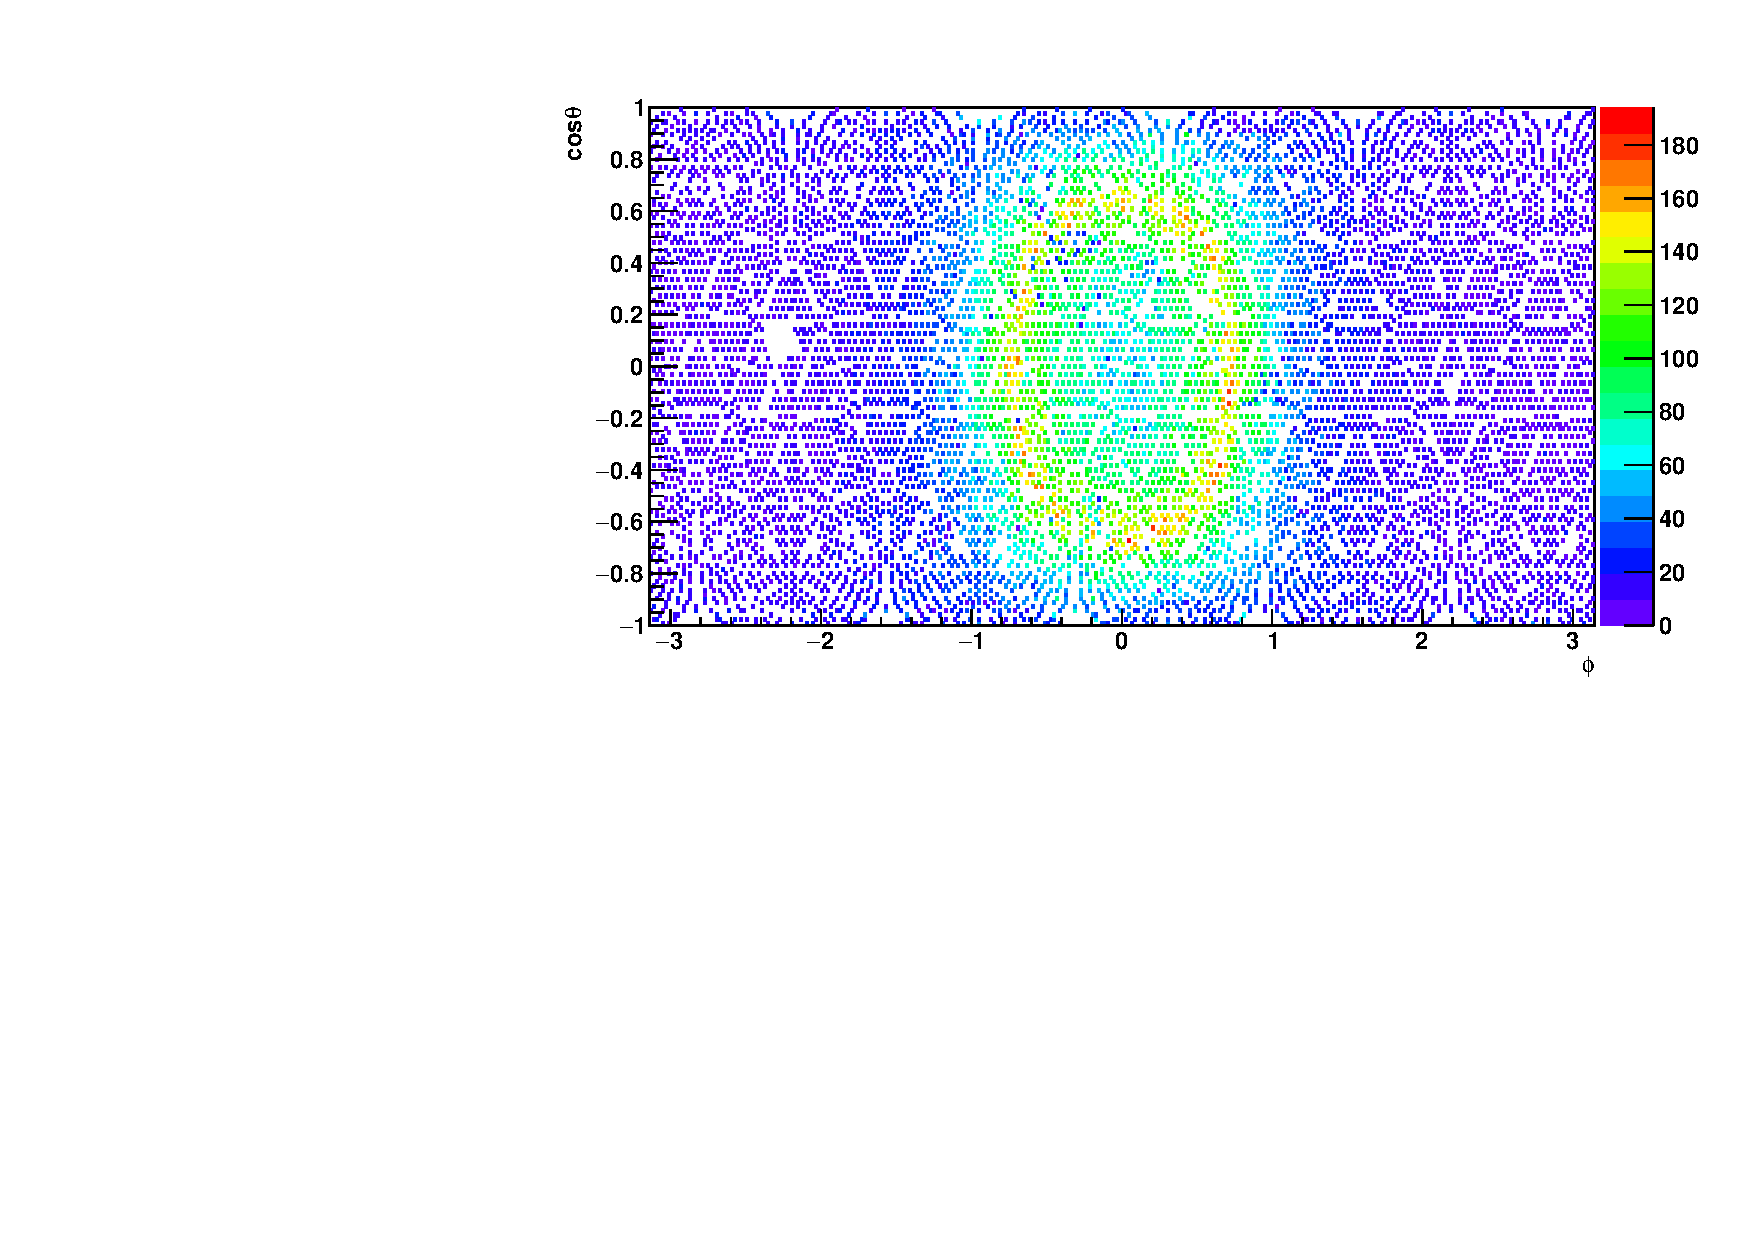
\includegraphics[width=7cm]{PMT_5MeVElectronWater.pdf}
	\end{minipage}
	\begin{minipage}[t]{0.48\textwidth}
		\centering
		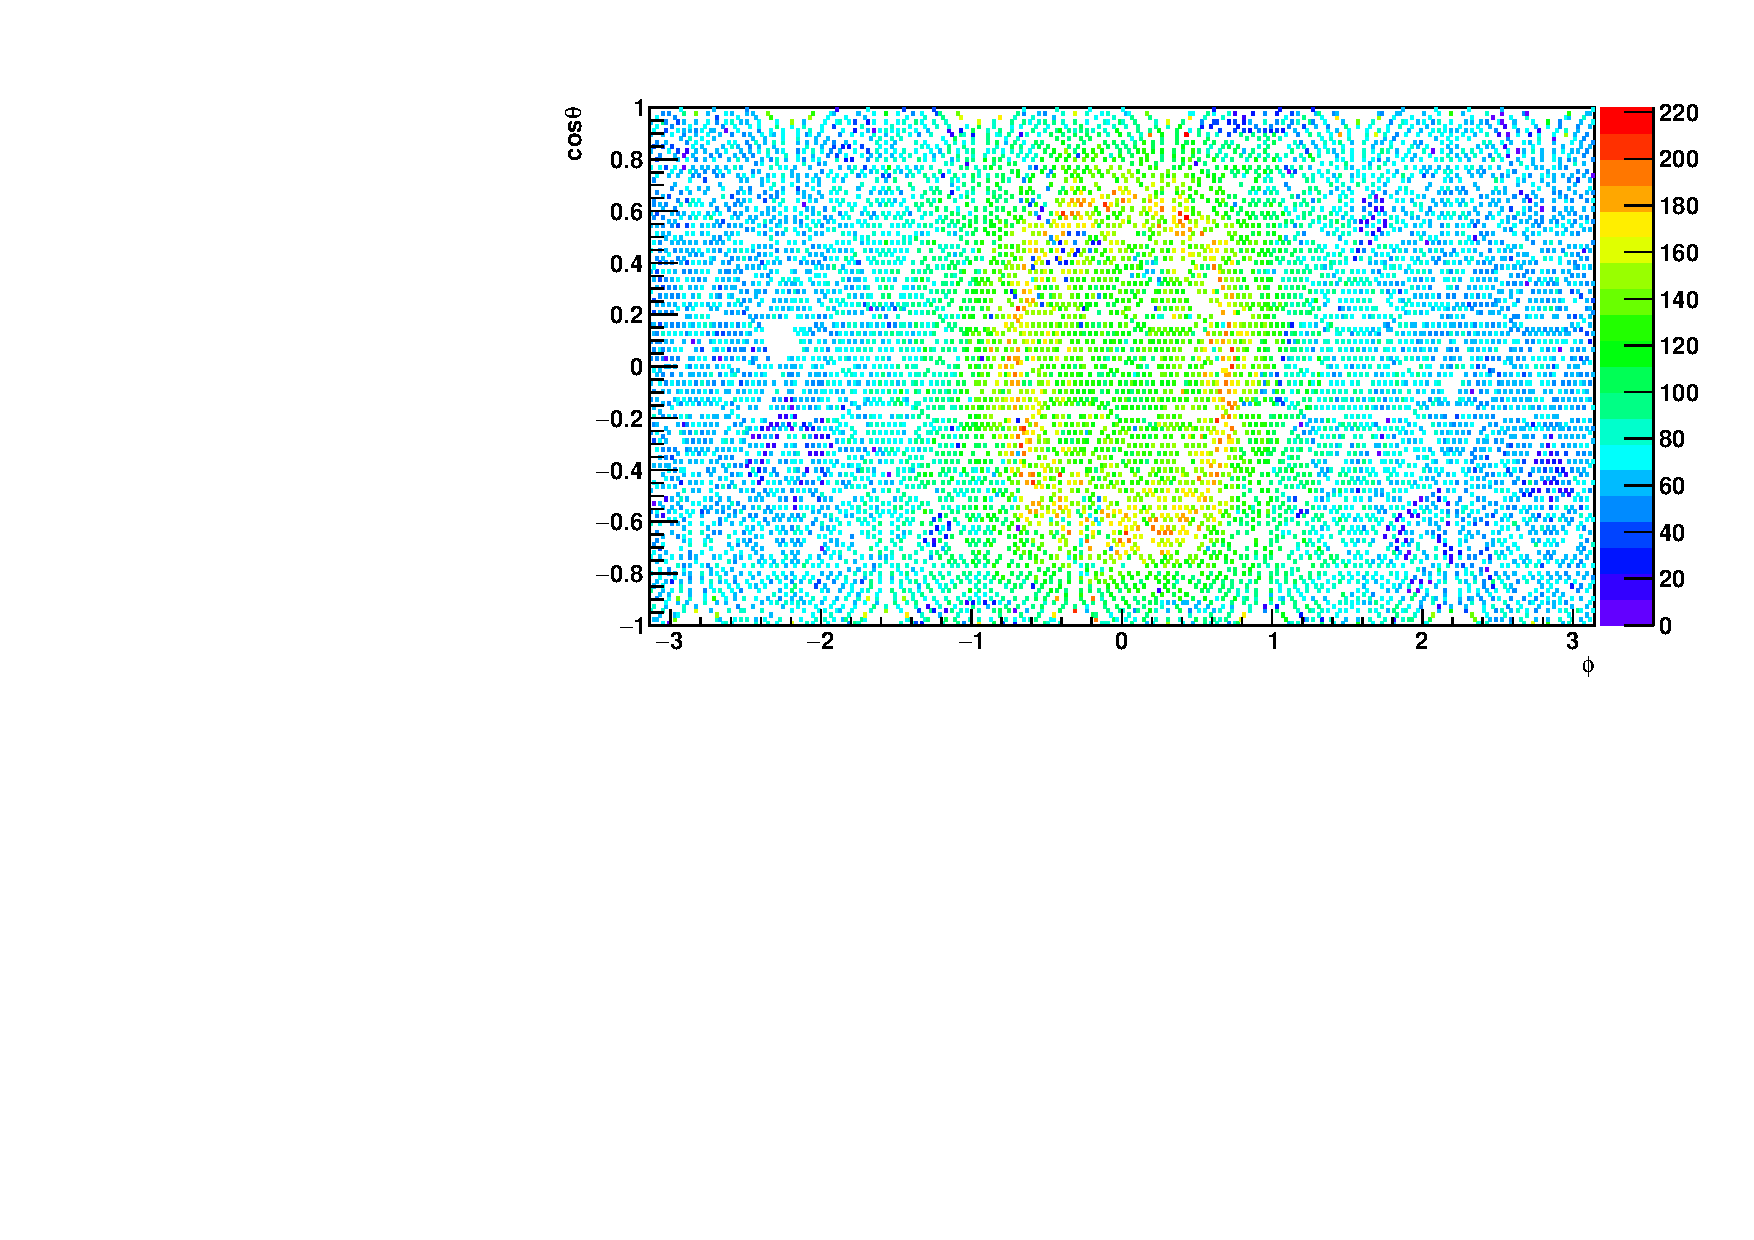
\includegraphics[width=7cm]{PMT_5MeVElectron0p1ppmPPO.pdf}
	\end{minipage}
	\caption[Position distributions of hit PMTs (in zenith and azimuth angles).]{Position distributions of hit PMTs (in zenith and azimuth angles) for 5 MeV electrons traveling along $+x$ direction in the pure water (left) and the water plus 0.1 ppm PPO (right).}
	\label{pmt_wls}
\end{figure}

Figure~\ref{nhit_wls} shows the energies of simulated electrons as a function of the mean value of the $\mathrm{NHit}$ distribution (mean NHits). In pure water, a 1 MeV electron simulation does not trigger any PMTs while in wbWLS case we have a mean NHits of 20.

\begin{figure}[htbp]
	\centering	
	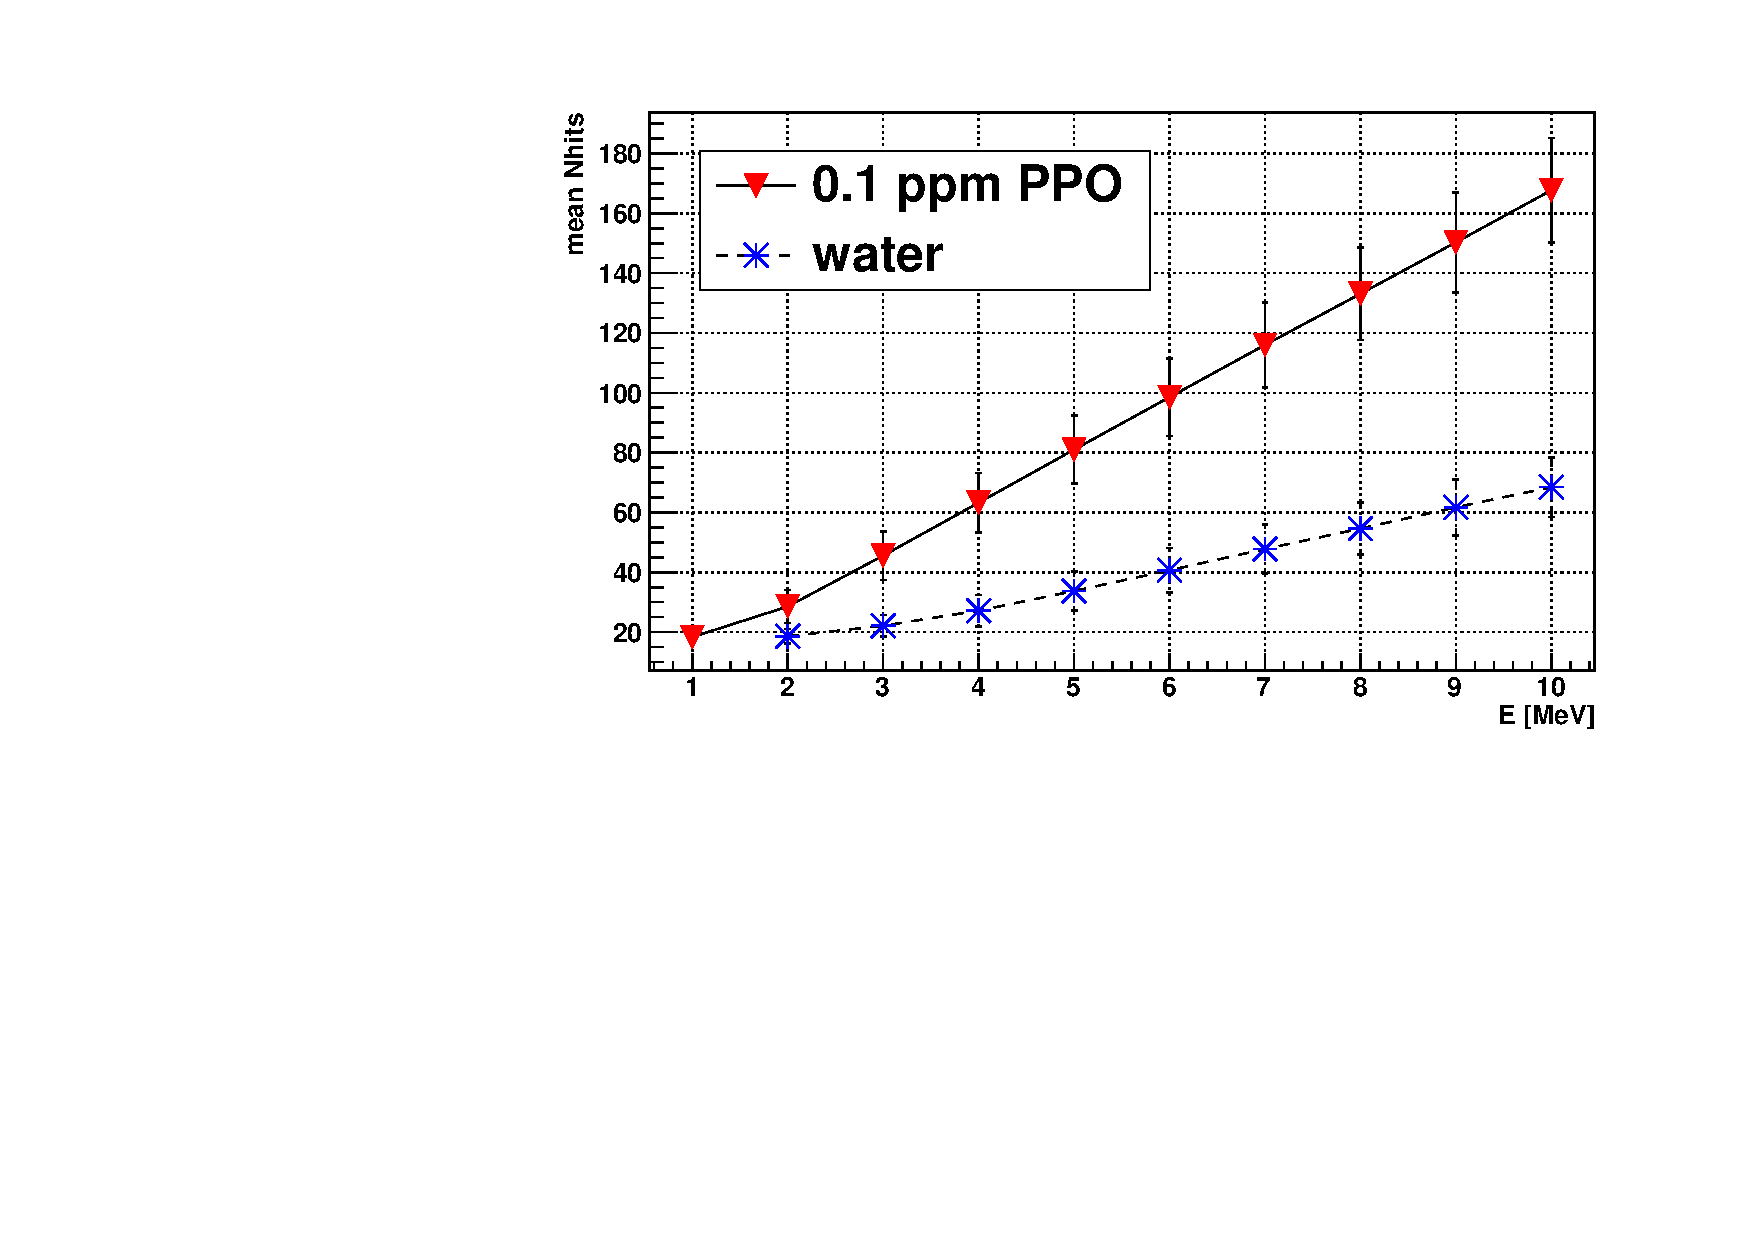
\includegraphics[width=9cm]{nhits_wls.pdf}
	\caption[The energies of simulated electrons as a function of mean NHits.]{The energies of simulated electrons as a function of mean NHits. The values in the 0.1 ppm PPO (solid line with inverted triangle) are compared with the water (dashed line with star).}
	\label{nhit_wls}
\end{figure}

In the wbWLS case, since the WLS absorbs and re-emits photons, the reconstruction mentioned in section \ref{sect:mpw} is slightly modified to build the MP WLS Fitter. According to the optical property of PPO, the prompt light emitted from an event has a probability of $\sim$0.6 to be absorbed by the WLS and then re-emitted at a shifted vertex along the particle direction $\hat{n}$. Then the fitter returns a shifted vertex, $\vec{X}_{0,shifted}=\vec{X}_0+\mathrm{offset}\cdot\hat{n}$. The offset we set in the fitter is 100 mm obtained from simulations. Figure~\ref{WLS_pdf} shows the timing $PDF$ for the wbWLS, which is the PMT response time modified to photon propagation time in the wbWLS.
\begin{figure}[htbp]	
	\centering		
	\begin{minipage}[b]{0.5\textwidth}			
		%\centering			
		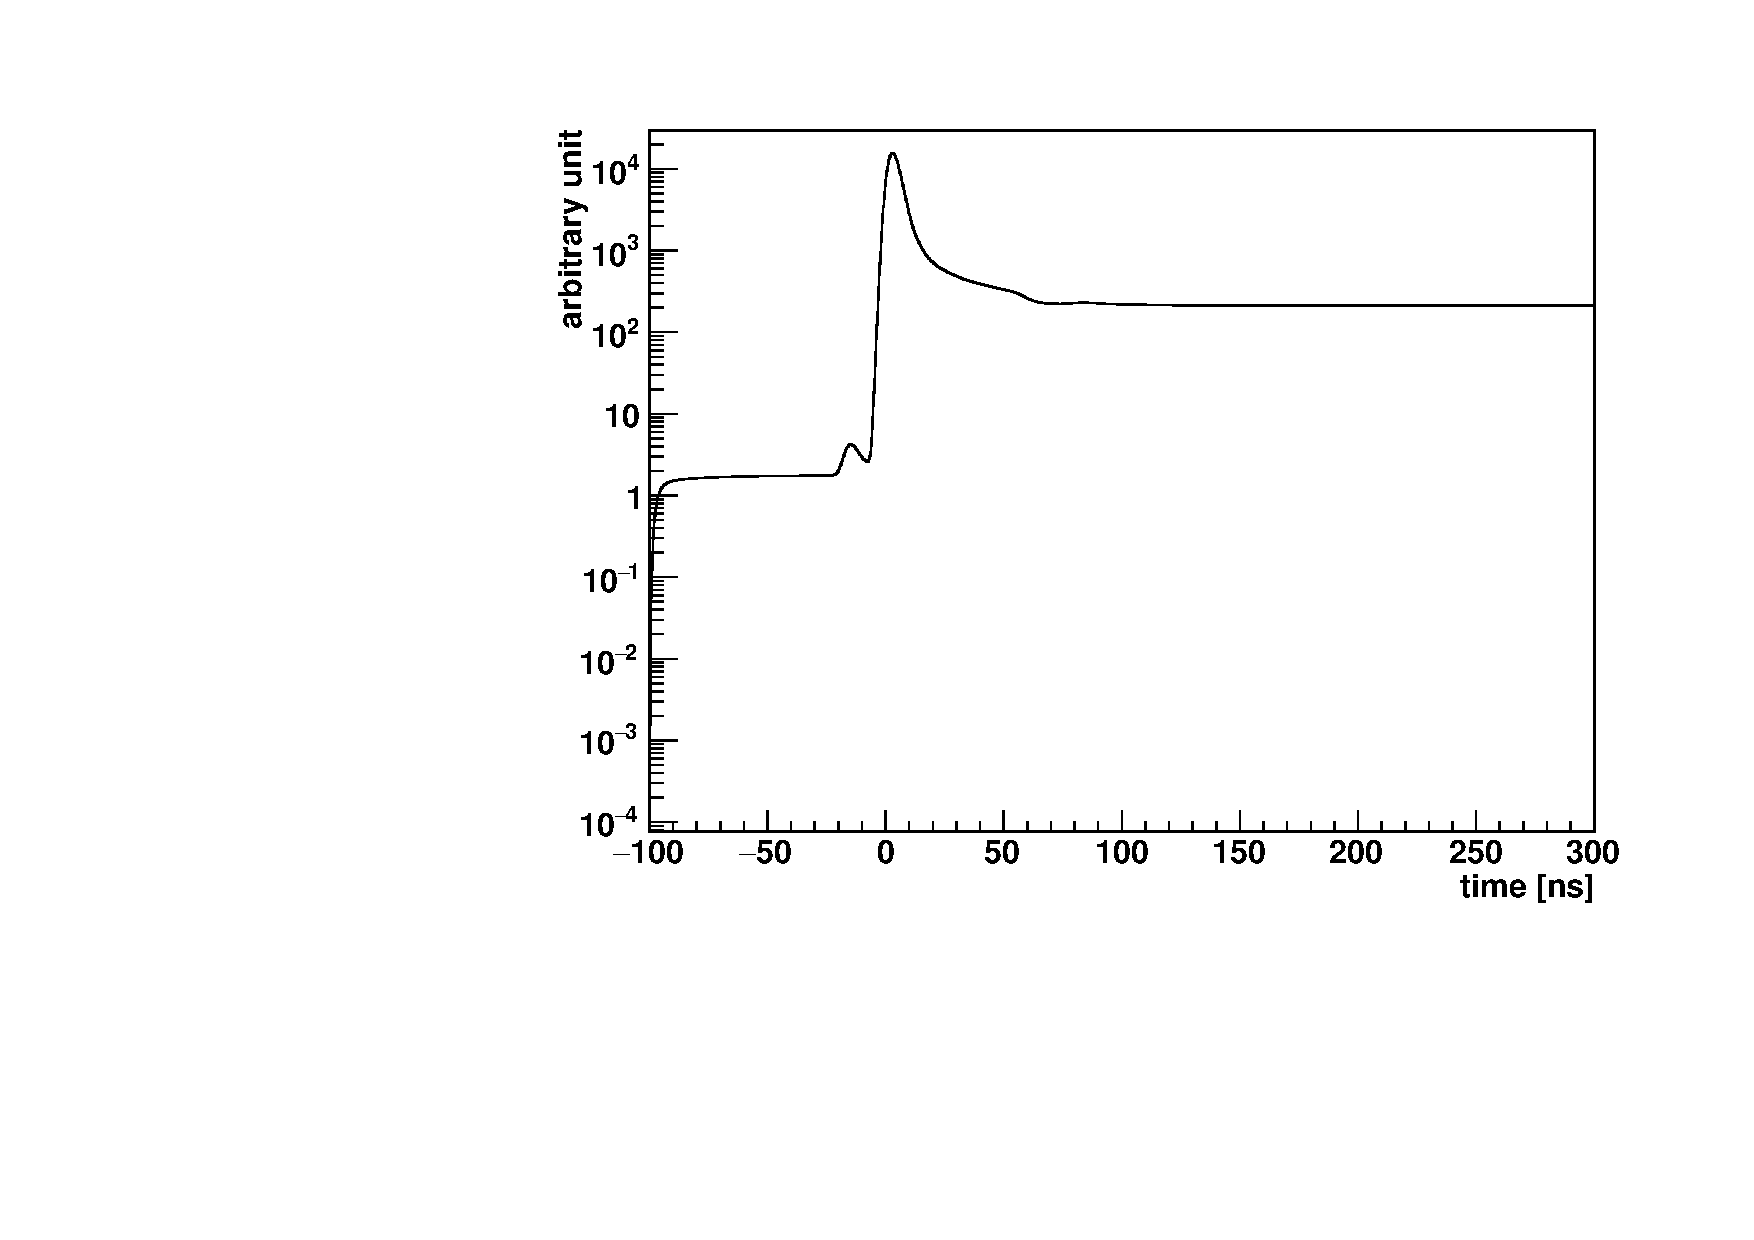
\includegraphics[height=6cm]{WLSTime_pdf.pdf}			
	\end{minipage}%				
%		\begin{minipage}[b]{0.5\textwidth}		
%			%\centering	
%			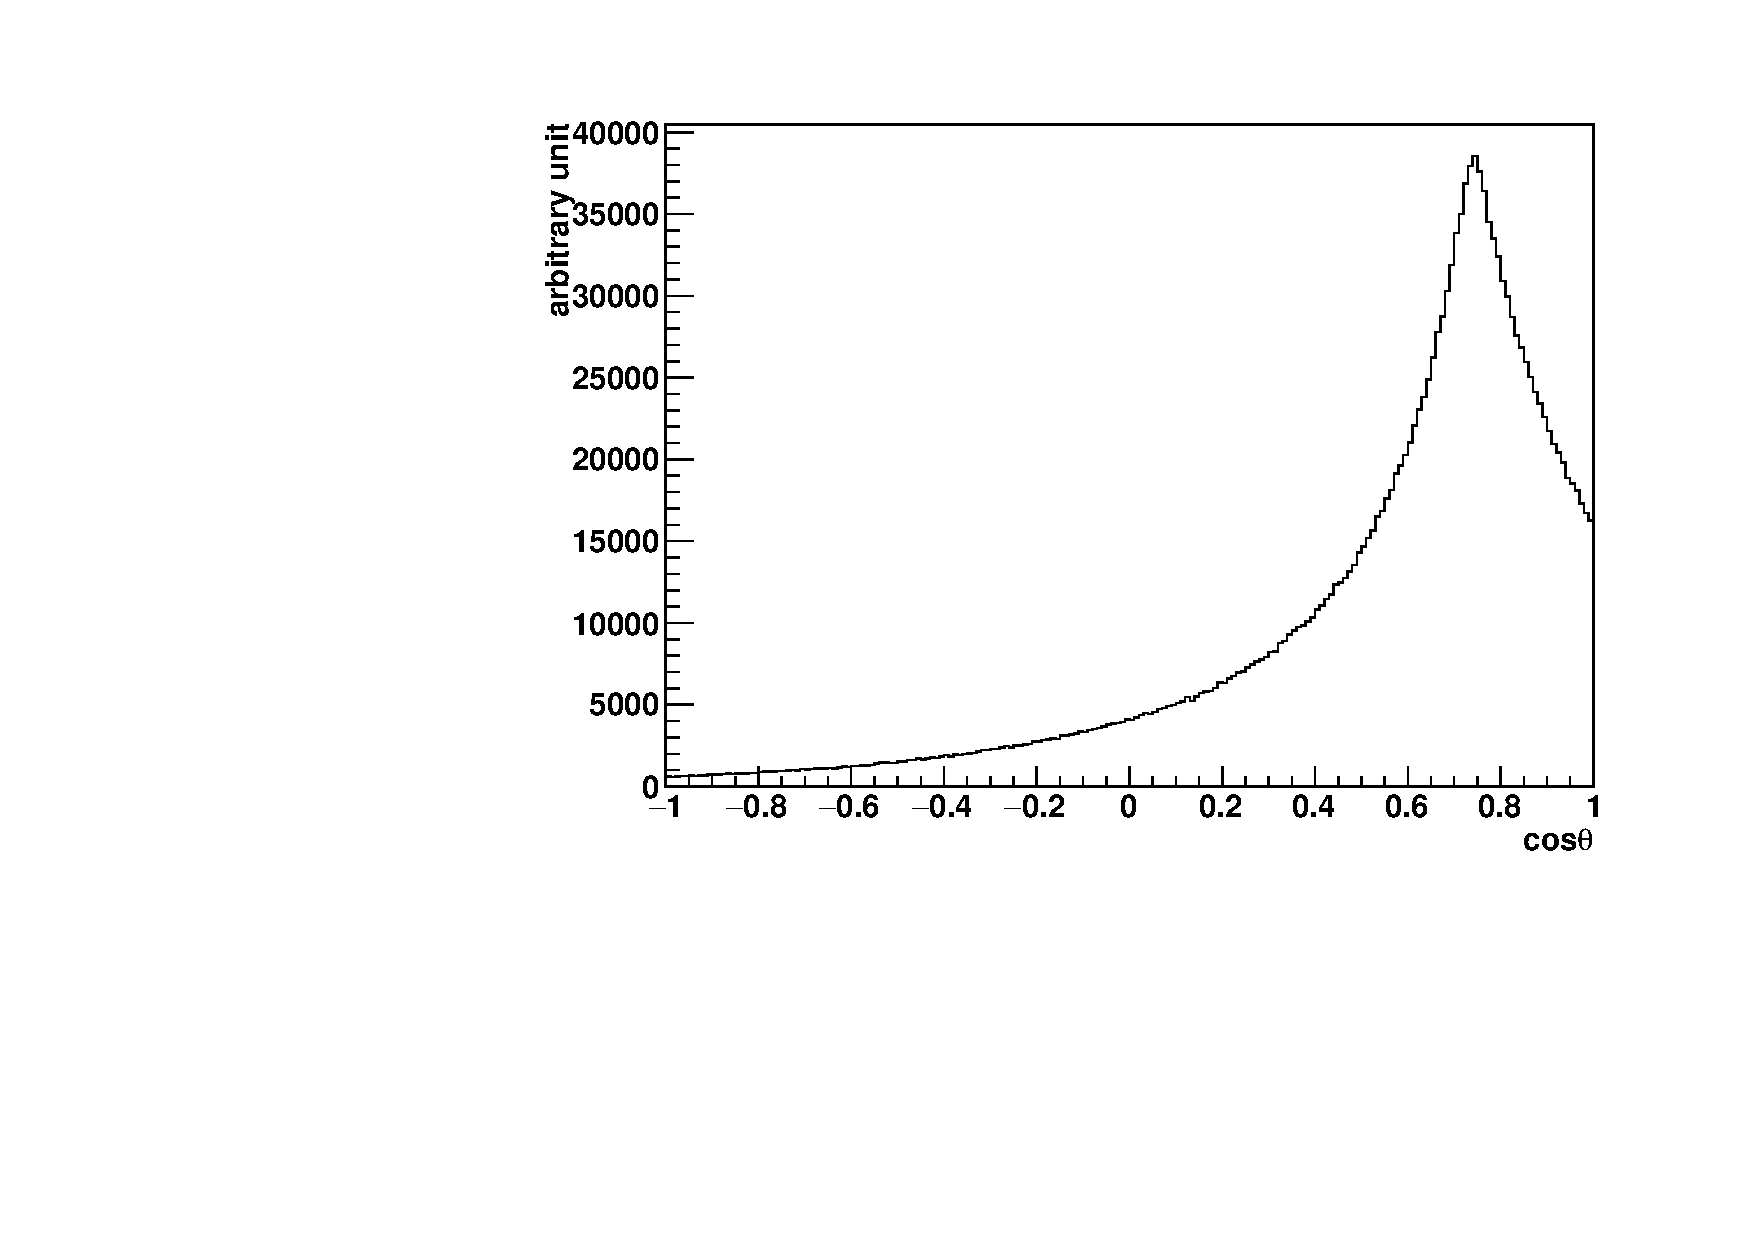
\includegraphics[height=5cm]{ChAngle_pdf.pdf}	
%		\end{minipage}	
	\caption{\label{WLS_pdf} The timing $PDF$ for the wbWLS.}	
\end{figure}

To reconstruct the direction, besides the angular distribution of Cherenkov photons, $\cos\theta_{Ch}$, we also consider the fraction of the re-emitted and wavelength shifted photons that cause a flat angular distribution.

To test the performance of the \texttt{MP WLS Fitter}, 5 MeV $e^-$ were simulated at the center of the AV filled with wbWLS and traveling along +x direction. As a comparison, the same simulation was done for the AV filled with pure water and the simulated events were reconstructed by the water fitter.

Fig.~\ref{WLSFitPos} shows the performance of the WLS fitter reconstructed positions of the MC simulations compared to the pure water case. For the fit position distribution of 5-MeV $e^-$ in the wbWLS, we get a root mean square (RMS) of 201 mm and a bias to the center (the mean of histogram) of 29 mm. Compared to the pure water case, the fit bias is about 19 mm better and the RMS is 188 mm better.

\begin{figure}[htbp]	
	\centering	\label{WLSFitPos} 		
	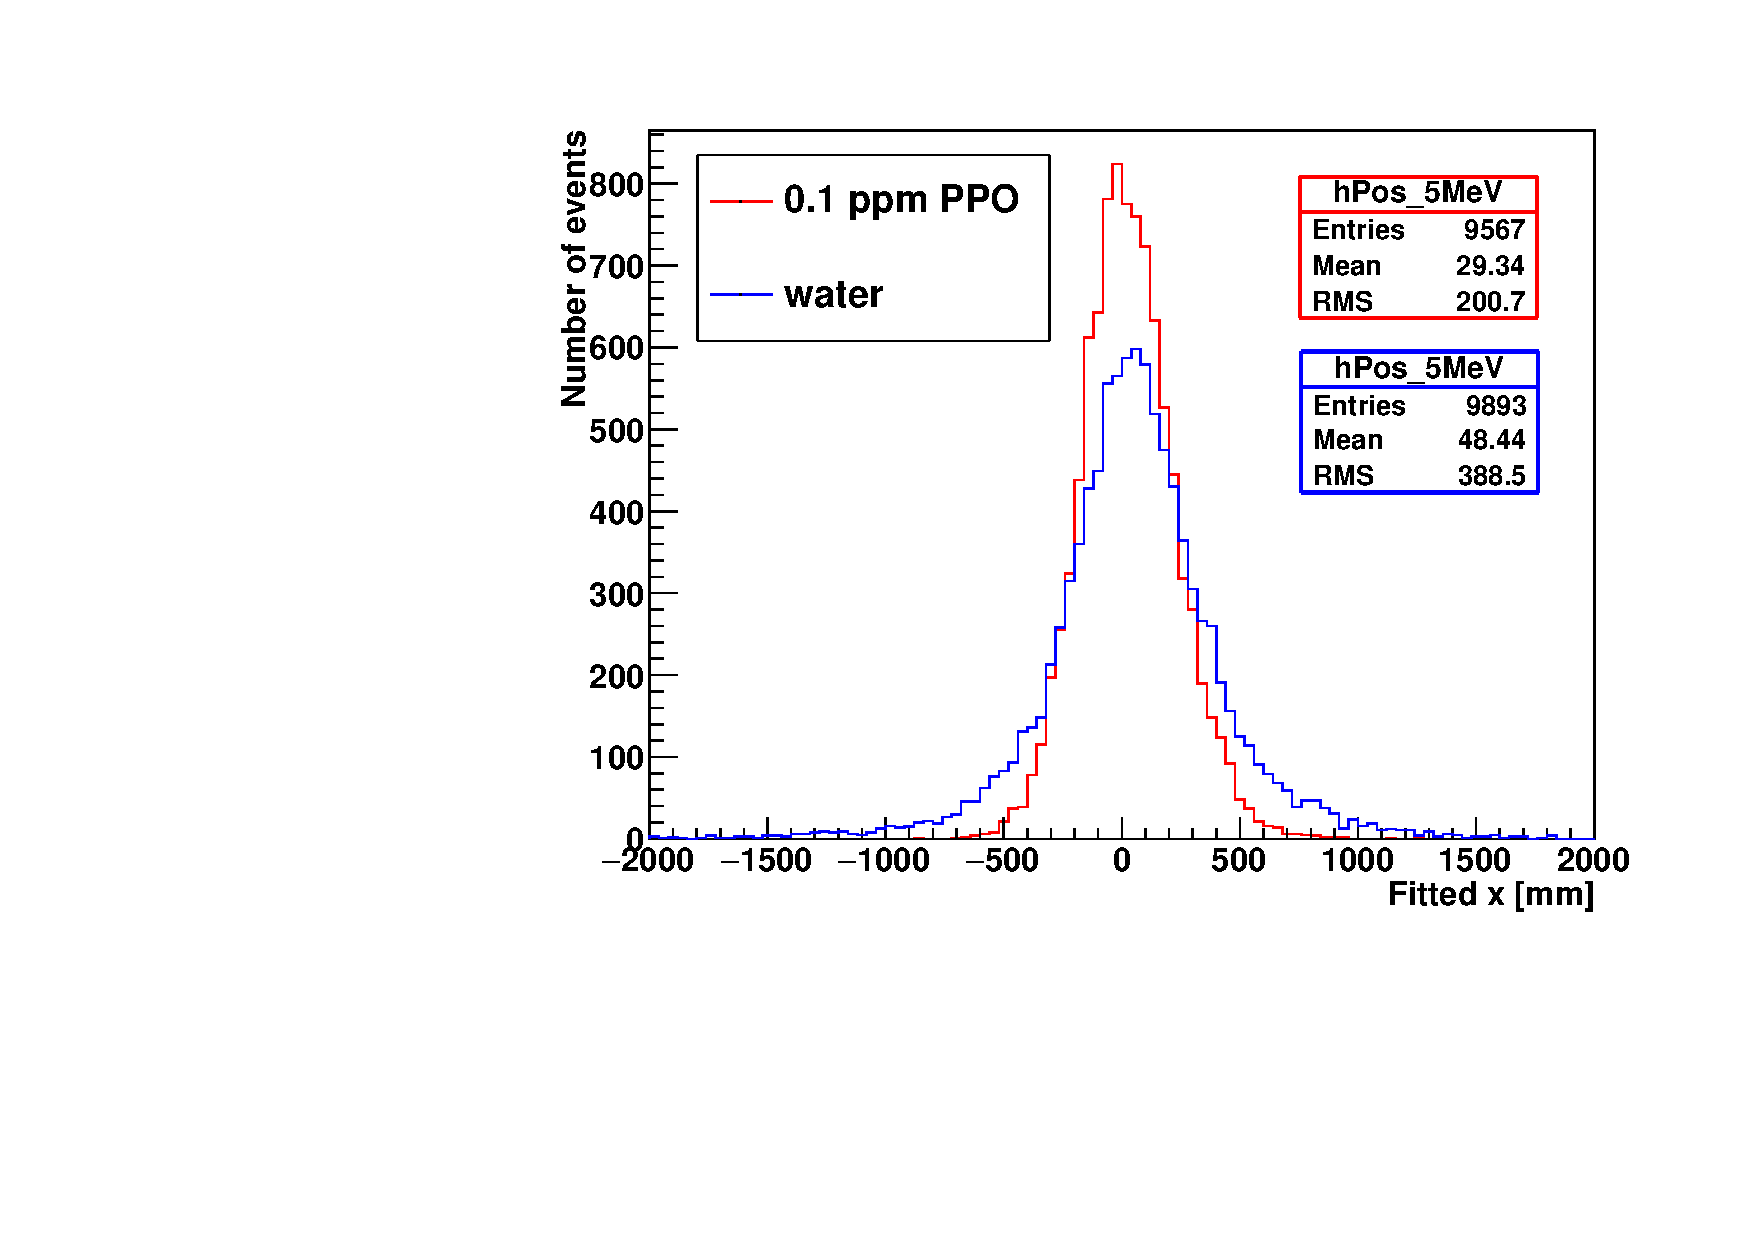
\includegraphics[height=5cm]{WLS_FittedPos.pdf}		
	\caption[Fitted x position.]{Fitted x position. The \texttt{MP WLS fitter} reconstructed $x$ positions of the 5-MeV $e^-$ events in the wbWLS (red) are compared to the ones in the water (blue).
	}
\end{figure}

Similar to Sect.~\ref{sect:directResol}, $\cos\theta_a$ in Eqn.~\ref{eq:cosTheta_fraction} is used to quantify the performances in direction reconstruction. Table.~\ref{tab:quantAngular} shows the results of $\cos\theta_{a}$ for SNO heavy water data\cite{boulay2004direct} and simulations for SNO+ pure water and wbWLS. It shows that the SNO+ pure water gives the best direction reconstruction, while the wbWLS is about 30\% off in $\cos\theta_{0.9}$ compared to the SNO+ pure water.
\begin{table}[ht]
	\caption{A comparison of quantitative estimates for the angular resolution for the SNO heavy water, SNO+ wbWLS and the SNO+ pure water cases.}\label{tab:quantAngular}
				\centering		
		\begin{tabular*}{120mm}{c@{\extracolsep{\fill}}cccc}
			\toprule 
			medium & $\cos\theta_{0.9}$ & $\cos\theta_{0.8}$ & $\cos\theta_{0.5}$
			\\
			\midrule
			SNO heavy water  & 0.50 & 0.71 & 0.92  \\	
			SNO+ water  & 0.62 & 0.78 & 0.98	\\
			wbWLS  & 0.37 & 0.63 & 0.90  \\	
			\bottomrule	
		\end{tabular*}
\end{table}

Comparing a pure water SNO+ detector and the wbWLS one, using the \texttt{MP WLS fitter} for physics events gives a better position resolution without a significant loss in the performance of the direction reconstruction. This \texttt{MP WLS fitter} was also applied in a study of the potential for measuring the reactor antineutrinos in the wbWLS-filled SNO+ detector, see Ref.~\cite{mekarski2018electron} for details.

\section{Vertex Reconstruction for the Partial-fill}\label{sect:partialFitter}
The following two sections discuss about the vertex reconstruction relating to the liquid scintillator. The vertex reconstructions for the partial-fill and scintillator phases are very similar. Both of them tackle with two detection media: the water and the scintillator, and calculate the light paths in these two regions. I will first describe the calculations in the partial-fill case, since its geometry is more complicated while the full scintillator case can be considered as a simplified version.

\subsection{Partial-fill}
In the partial-fill geometry, the SNO+ detector can be described as a composition of three parts: the neck cylinder filled with the scintillator; the AV sphere, which is split by a water-scintillator interface (plane) inside, and above this plane is the scintillator and below is the water; and the PSUP sphere outside the neck and the AV, filled with the water.

Omitting the acrylic and other detector materials, photons mainly pass through two different media: the water and the scintillator. As shown in Fig.~\ref{fig:scintpath}, assuming a straight light path from a vertex to a hit PMT position, its total length is $|\vec{l}_p|=|\vec{X}_\mathrm{PMT}-\vec{X}_0|$. The \texttt{MP partial fitter} evaluates the length of the $|\vec{l}_p|$ in the scintillator: $d_{sp}$ and then the length in the water is $|\vec{l}_p|-d_{sp}$. Since photons travel at different speeds in these two media: $v_{gr,scint}$ and $v_{gr,water}$, the \texttt{MP partial fitter} evaluates the time of flight, $t_{transit}$ by:
\begin{equation}
t_{transit} = \frac{|\vec{l}_p|-d_{sp}}{v_{gr,water}} +\frac{d_{sp}}{v_{gr,scint}},
\end{equation}
and thus the time residual, $t_{res}$ is calculated. Once the $t_{res}$ is obtained, the following fitting procedure is the same to the \texttt{MP water fitter}.

\begin{figure}[!htb]
	\centering
	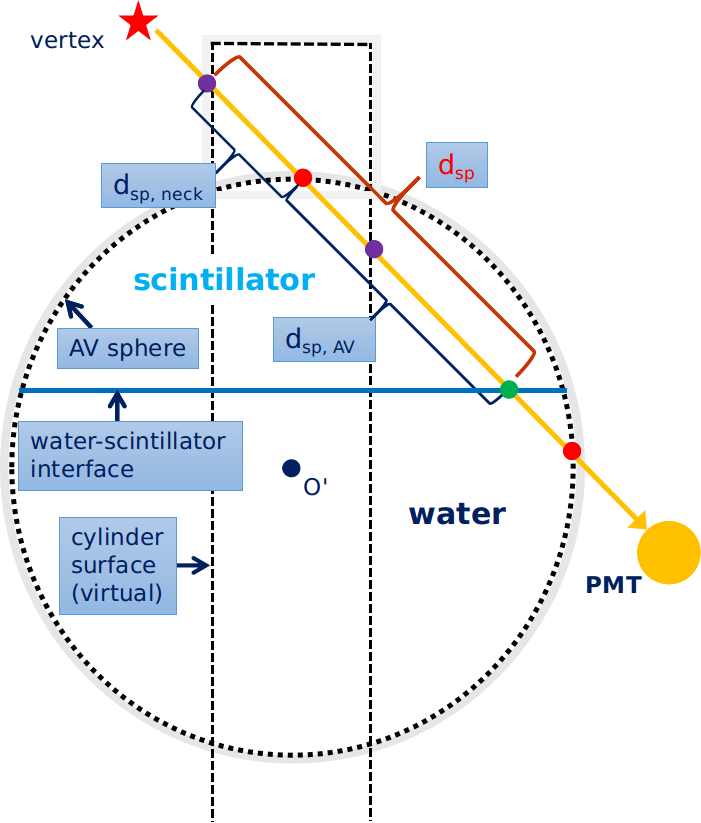
\includegraphics[width=7cm]{scintpath.png}
	\caption[Light path calculation for the \texttt{MP partial fitter}.]{Light path calculation for the \texttt{MP partial fitter}. In the figure, a light path intersects with the neck cylinder surface, the AV sphere as well as the water-scintillator interface. The total length of the path in the scintillator region (scintillator path, $d_{sp}$) includes the paths in the neck ($d_{sp,neck}$) and in the AV ($d_{sp,AV}$). Calculations of the ray-cylinder, ray-plane and ray-sphere intersections are applied.}
	\label{fig:scintpath}
\end{figure}

Therefore, the crucial part here is to calculate the $d_{sp}$. The light path $\vec{l}_p$ is considered as a ray with a direction (rather than a line without direction). The ray intersects with three geometry objects: the neck cylinder, the AV sphere and the water-scintillator interface plane. As illustrated in Fig.~\ref{fig:scintpath}, a detailed calculation of $d_{sp}$ includes the evaluations of (1) $\vec{l}_p$ and neck (ray-cylinder) intersection; (2) $\vec{l}_p$ and the AV (ray-sphere) intersection and (3) $\vec{l}_p$ and the water-scintillator interface (ray-plane) intersection. The $d_{sp}$ is further separated into the path lengths in the neck ($d_{sp,neck}$) and in the AV ($d_{sp,AV}$). 

For a trial position $\vec{X}_0=(x_0,y_0,z_0)$ and a hit PMT position $\vec{X}_{\mathrm{pmt}}=(x_\mathrm{pmt},y_\mathrm{pmt},z_\mathrm{pmt})$, define the ray vector as $\vec{l}_0\equiv\vec{X}_0+a\cdot \vec{u}$, where $a$ is the distance between vertex and intersection point and it is the parameter to be determined; $\vec u=\frac{\vec{X}_{\mathrm{pmt}}-\vec{X}_0}{|\vec{X}_{\mathrm{pmt}}-\vec{X}_0|}$ is the direction of the ray vector. It is a unit vector pointing from the $\vec{X}_0$ to the $\vec{X}_{\mathrm{pmt}}$. The following goes through the three intersection cases:

\begin{itemize}
\item Ray-sphere intersection

In the ray-sphere intersection case (ray vector passes through the AV sphere), the intersection points on the $\vec{l}_0$ satisfy the sphere equation $(\vec{X}-\vec{O}_{av})^2= r^2_{AV}$, where $\vec{O}_{AV}$ is the origin of the AV sphere and $\vec{O}_{AV} = (0,0,108)$ mm in the PSUP coordinate; $r_{av}=6005$ mm. Thus the intersection equation is:
$(\vec{l}_0-\vec{O}_{av})^2 = r^2_{AV}$.

Let $\Delta \equiv {[(\vec{X}_0-\vec{O}_{av})\cdot\vec{u}]}^2-{(\vec{X}_0-\vec{O}_{av})}^2+r^2_{av}$, if $\Delta>0$, solve the equation and get:
\begin{equation}\label{eq:ray-sphere}
a_{\pm} = -(\vec{X}_0-\vec{O}_{av})\cdot\vec{u}\pm\sqrt{\Delta},~if~\Delta>0.
\end{equation}
In this case, both $a_+$ and $a_-$ exist and their values are different. If $a_+>a_->0$, the length of the path inside the sphere is $a_+-a_-$, as illustrated in Fig.~\ref{line-sphere} (a). Due to this geometry, the event position should be outside the AV, the condition $|\vec{X}_0|\geq r_{AV}$ is automatically met. If $a_+>0>a_-$, $a_-$ determines the intersection point along the opposite direction of the ray vector. Thus the ray vector actually does not pass that point (different to the line intersection with no direction). Thus the length of the path inside the sphere is $a_+$, as illustrated in Fig.~\ref{line-sphere} (b). Also, the condition $|\vec{X}_0|<r_{AV}$ is automatically met. 

If $\Delta\leq0$,
there is no intersection point or only one intersection point (when $\Delta=0$) at the AV, the ray vector never passes through the AV sphere, as illustrated in Fig.~\ref{line-sphere} (c) and (d).

\begin{figure}
	\centering
{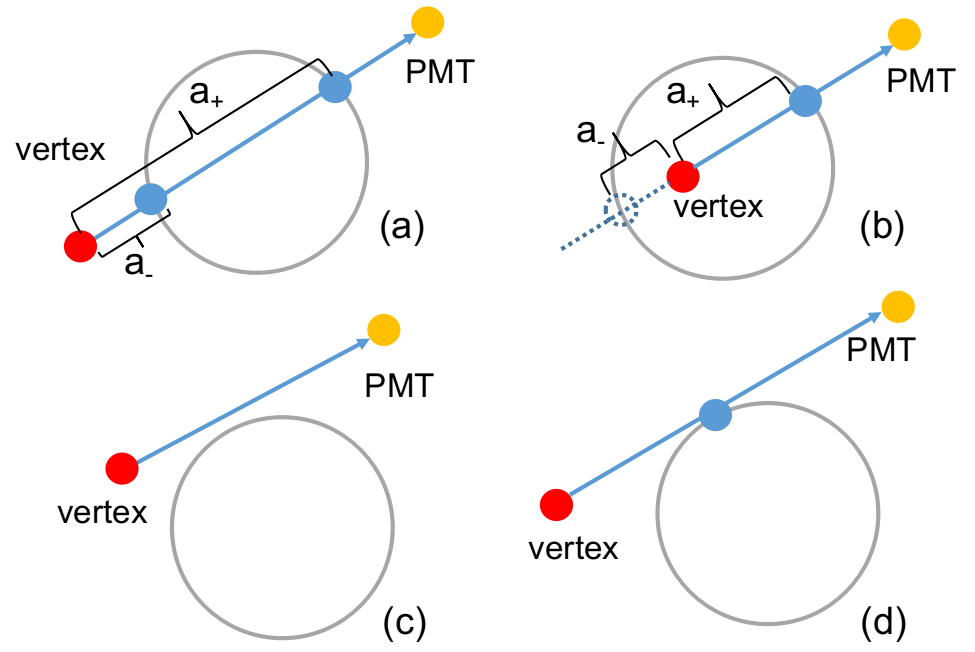
\includegraphics[width=80mm]{line-sphere.png}}
\caption{Line-sphere intersections. (a) the ray vector intersects the sphere with 2 points; (b) the ray vector intersects the sphere with 1 point; (c) and (d): the ray vector never passes through the sphere.}\label{line-sphere}
\end{figure}

\item Ray-plane intersection

For the ray-plane intersection, the z components of the intersection points on $\vec{l}_0$ satisfy the plane equation $z=Z_{split}$, where $Z_{split}$ is the water level, i.e., the z position of the water-scintillator intersection. Thus the intersection equation is:
$l_{0,z}=Z_{split}$, where $l_{0,z}=z_0+a\cdot u_z$.

If $u_z=z_\mathrm{pmt}-z_0=0$, the ray is parallel to the plane and never intersects the plane.

If $u_z\neq 0$, solve the equation, we have: $a=(Z_{split}-z_0)/u_z=(Z_{split}-z_0)$.
Let: 
\begin{equation}
a_3 \equiv a = \frac{(Z_{split}-z_0)|\vec{X}_{\mathrm{pmt}}-\vec{X_0}|}{z_\mathrm{pmt}-z_0}~~(if ~z_\mathrm{pmt}-z_0\neq 0),
\end{equation}

Similar to the case of ray-sphere intersection, if $a_3<0$, the ray-plane intersection point is on the extended line along the opposite direction to the ray; $a_3 \geq 0$ ensures the ray hits the interface. Note that here we consider the plane is infinitely large. Later we will combine with the calculations of the other geometries to cut it off. 

\item Ray-cylinder intersection

For the ray-cylinder intersection, the x and y components of the intersection points on the $\vec l_0$ satisfy the intersection equation: $l^2_{0,x}+l^2_{0,y} = r^2_{neck}$, where $r_{neck}$ is the radius of the neck cylinder ($r_{neck}=785~mm$).

To solve the equation,  let: $\Delta'\equiv [x_0\cdot (x_{PMT}-x_0)+y_0\cdot(y_{PMT}-y_0)]^2 - ( x_0^2+y_0^2-r^2_{neck})\cdot [(x_{PMT}-x_0)^2+(y_{PMT}-y_0)^2]$, and then we get: 
\begin{equation}\label{eq:ray-cylinder}
a'_{\pm} = |\vec{X}_{PMT}-\vec{X}_0|\cdot\frac{-[x_0\cdot (x_{PMT}-x_0)+y_0\cdot(y_{PMT}-y_0)] \pm \sqrt\Delta' }{(x_{PMT}-x_0)^2+(y_{PMT}-y_0)^2},~if~\Delta'>0,
\end{equation}

Similar to the ray-sphere case, if $a'_{+}>a'_->0$, the length of the path inside the cylinder is $a'_+-a'_-$. Due to this geometry, the event position should be outside the cylinder, the condition $(x^2_0+y^2_0)\geq r_{neck}$ is automatically met. If $a'_+>0>a'_-$, the event position should be inside the cylinder and the ray-vector intersects the cylinder with one point (while the other point is along the opposite direction). Thus the length of the path inside the cylinder is $a'_+$. If $\Delta'\leq0$, the ray vector never passes through the neck cylinder. Also note that here we consider the cylinder is infinitely long. This will also be cut off by the combined calculations of the other geometries. In addition, since only the neck region inside the PSUP is valid for the fitter, we should also ensure $z<8390~mm$ (in the PSUP coordination).

\end{itemize}

To evaluate the length of the $|\vec{l}_p|$ in the scintillator region ($d_{sp}$), the above three geometries needs to be combined carefully. The following two procedures go through all the possible situations. First combine the evaluations of the ray-sphere and the ray-plane intersections to calculate the light path in the AV scintillator region ($d_{sp,AV}$). Then combine the evaluations of the ray-sphere and the ray-cylinder intersections to calculate the light path in the neck scintillator region ($d_{sp,neck}$). Detailed algorithms are shown in Appendix.~\ref{appendix:lightpath}.

Since the valid fit requires the events inside the PSUP sphere, only the neck region inside the PSUP sphere (with $6108<z_{neck}<8390~mm$) needs to be considered. The neck path calculation is also allowed to be turned off, while a worse fitted result is expected. Detailed calculations are shown in Appendix.~\ref{appendix:lightpath}.

If $d_{sp}=0$, the light path is always in the water. In this case, the fitter is the same to the \texttt{MP water fitter}. It fits the vertex with the \texttt{MP water fitter} $PDF$. Once the light path passes through the scintillator region, the fitter fits with a scintillator timing $PDF$, in which the PMT time response was modified to photon propagation time in scintillator, as shown in Fig.~\ref{partialpdf}.

\begin{figure}[htbp]
	\centering	
	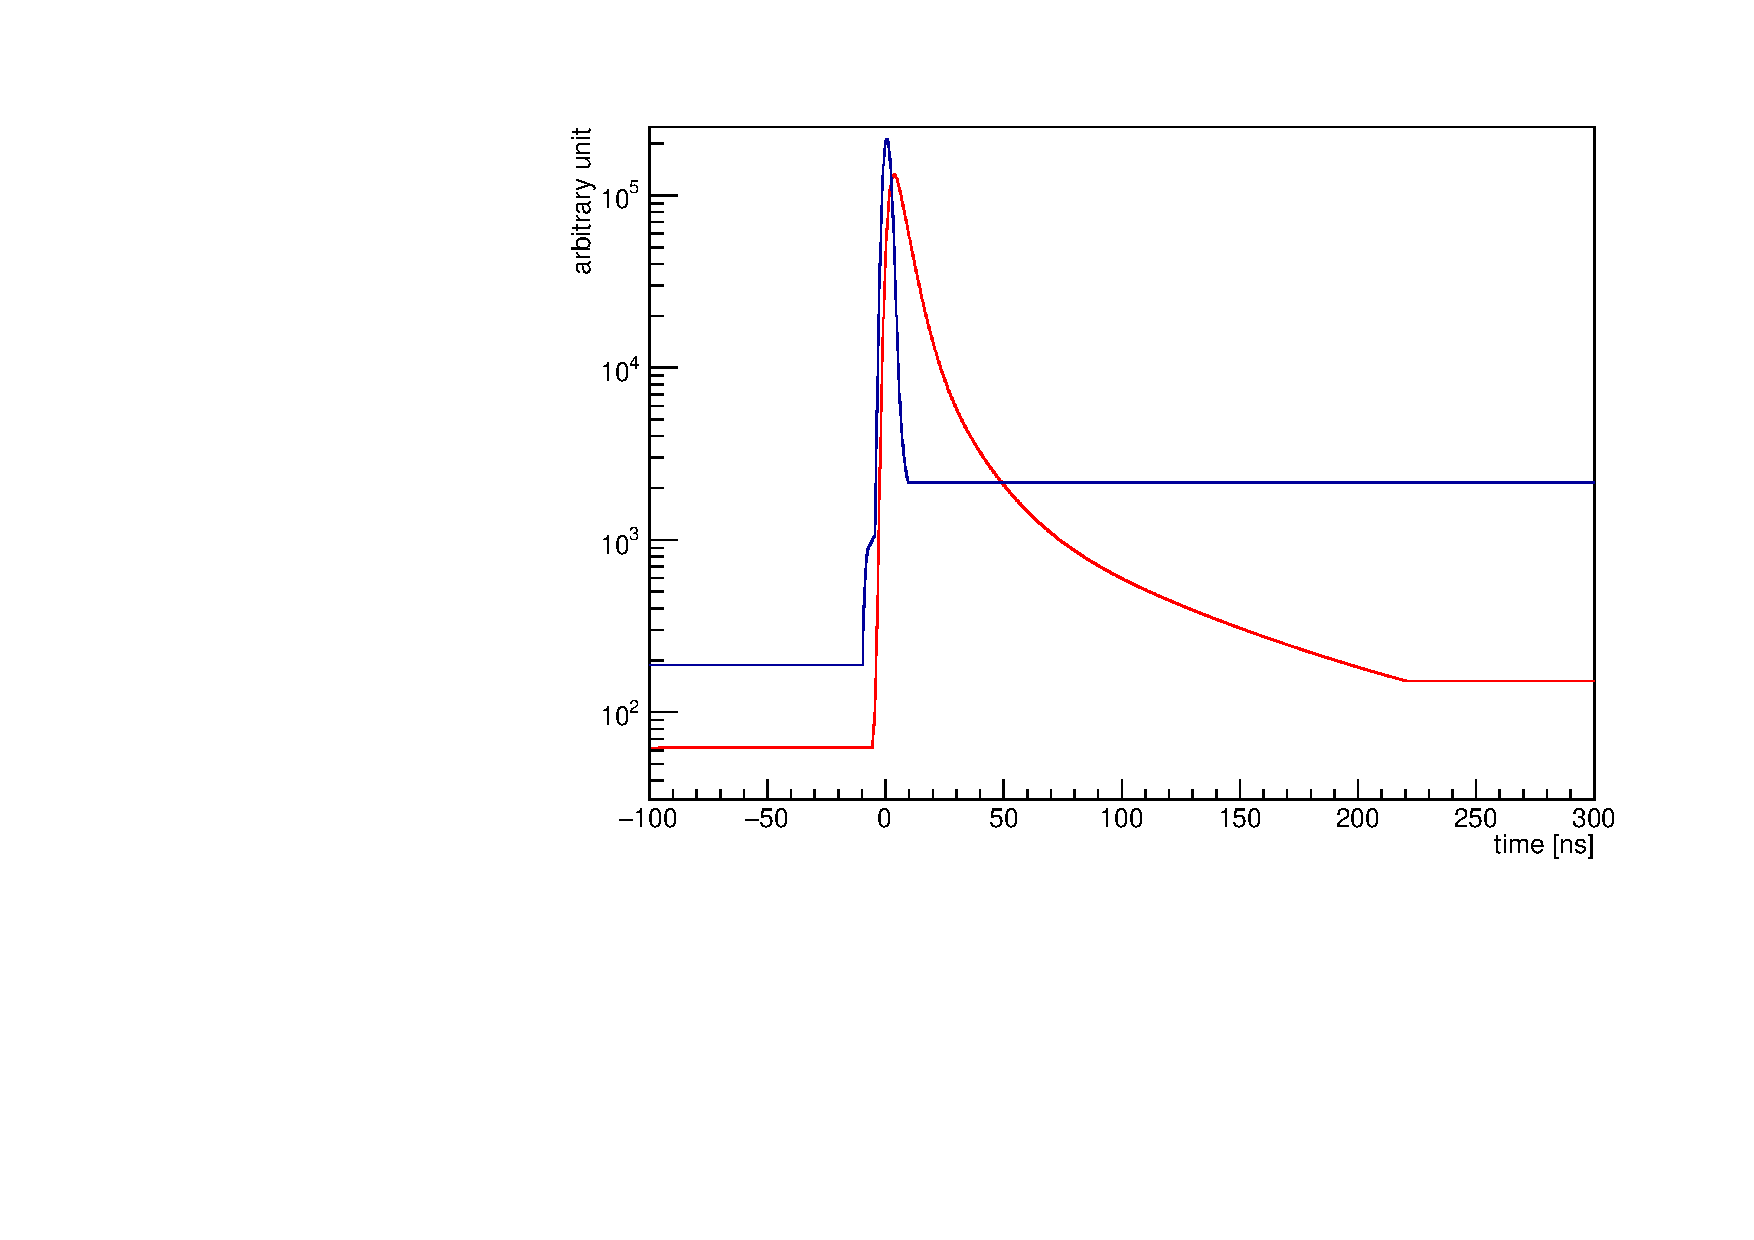
\includegraphics[width=7cm]{scintpdf.pdf}
	\caption[The timing $PDF$s used by the \texttt{MP partial fitter}.]{The timing $PDF$s used by the \texttt{MP partial fitter}. Blue: the timing $PDF$ used by the \texttt{MP water fitter}; red: the scintillator timing $PDF$.}
	\label{partialpdf}
\end{figure}

The next section will discuss the timing $PDF$s used by the fitter.

\subsection{Making Timing $PDF$s}

\subsubsection{Different PPO Concentrations during the Filling}
During the partial-fill phase, the water level and the concentration of the PPO were changing. The PPO was gradually added into and mixed with the LAB, and for the relative stable partial-fill stages which were used for taking and analyzing data, the PPO concentrations dissolved in the LAB were 0.25 g/L (earlier stage from 2019 to 2020) or 0.5 g/L (later stage from 2020 to 2021). The planned concentration of the PPO in the scintillator phase is 2 g/L.

An understanding of the characteristic photon emission response is crucial for building the timing $PDF$ for the reconstruction. The Oxford group from the SNO+ collaboration did several bench-top measurements to obtain the time constants and relative light yields of the LAB sample dissolved with the following PPO concentrations: 0.25, 0.5, 1.0, 2.0 and 6.0 g/L\cite{oxfordMeasurement0,oxfordMeasurement}.

The emission time profile model used by the Oxford group is\cite{oxfordMeasurement}: 
\begin{equation}
f_{optics}(t)=\sum_{i=1}^3 (A_i\frac{e^{-\frac{t}{\tau_i}}-e^{-\frac{t}{\tau_{rise}}}}{\tau_i-\tau_{rise}})+A'\frac{e^{-\frac{t}{\tau_{rise}}}}{\tau_{rise}},
\end{equation}
where $A_i$ is the fraction of scintillation light emitted in the $i^{th}$ component, $\tau_i$ is the decay constant in the $i^{th}$ component, $\tau_{rise}$ is the rise time of scintillator.

The measured parameters are listed in Table.~\ref{tab:measureAmplitude} and Table.~\ref{tab:measureLightYield}.
\begin{table}[ht]
	\centering\label{tab:measureAmplitude}
	\caption{\label{oxfordMeasure} Time constants and amplitudes measured by Ref.~\cite{oxfordMeasurement}. Here the relative light yield is with respect to the LAB+2 g/L PPO case (11900 photons/MeV).}	
	{\centering
		\begin{tabular*}{160mm}{c@{\extracolsep{\fill}}ccccccccc}
			\toprule 
			PPO [g/L] & $\tau_{rise}$ [ns] & $\tau_1$ [ns] & $\tau_2$ [ns] & $\tau_3$ [ns] & $A_1$ [\%]  & $A_2$ [\%]   & $A_3$ [\%]  & $A'$ [\%] \\
			\midrule
			0.25 & 1.25 & 8.1 & 25.0 & 68.2 & 29.2 & 53.1 & 13.9 & 3.8\\
			0.5  & 1.12 & 7.2 & 18.7 & 49.1 & 43.5 & 40.4 & 12.6 & 3.5 \\
			1.0 & 1.18 & 5.5 & 13.3 & 40.9 & 45.6 & 37.5 & 13.3 & 3.6 \\
			2.0 & 1.06 & 4.2 & 11.7 & 48.9 & 57.9 & 27.8 & 8.9 & 5.4	\\
			6.0 & 0.94 & 2.5 & 9.3  & 46.0 & 63.7 & 17.0 & 8.6 & 10.7\\
			\bottomrule	
		\end{tabular*}
	}
\end{table}
\begin{table}[ht]
	\centering\label{tab:measureLightYield}
	\caption{\label{oxfordMeasure2}Relative light yield (RLY) measured by Ref.~\cite{oxfordMeasurement}.}	
	{\centering
		\begin{tabular*}{60mm}{c@{\extracolsep{\fill}}cc}
			\toprule 
			PPO [g/L] & RLY \\
			\midrule
			0.25 & 0.57\\
			0.5 & 0.65\\
			1.0 & 0.9\\
			2.0 & 1.0\\
			6.0 & 0.93\\
			\bottomrule	
		\end{tabular*}
	}
\end{table}
These Oxford-measured  time profiles were convolved with the PMT time response profile mentioned in Sect.~\ref{sect:waterVertex}, Fig.~\ref{fig:MPW_timingPDF}, to make the timing $PDF$ for the partial-fill vertex reconstruction. 
\begin{equation}\label{eq:OxfordTimingPDF}
f(t)_{PDF} = f_{optics}(t)\otimes f_{PMT~response}(t-t'),
\end{equation}

I wrote a python tool to create the timing $PDF$s to re-coordinate the partial fitter for the different PPO concentration cases\cite{partialFitterPDF}, as shown in Fig.~\ref{fig:oxfordPdf}.
\begin{figure}[!htb]
	\centering
	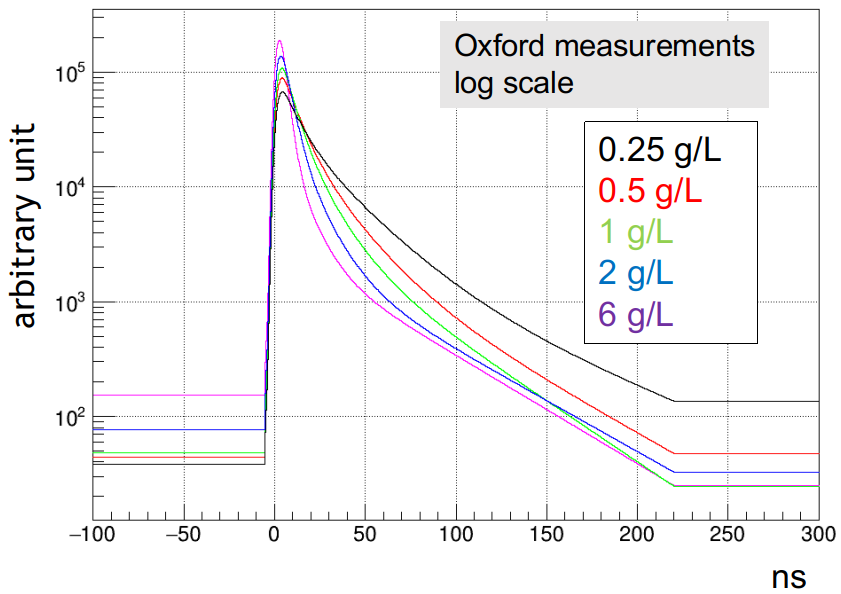
\includegraphics[width=10cm]{oxfordPdf_log.png}
	\caption{Timing $PDF$s built for various PPO concentrations based on the Oxford bench-top measurements.}
	\label{fig:oxfordPdf}
\end{figure}

% 2 g/L case: \ref{transfer_efficiency}\cite{collaboration2020development}. 
%Based on these measured parameters, $PDF$s were built. 

$PDF$s for all timing Sect.~\ref{sect:LS_SNO+}.

Following the same method of tuning the $v_{gr,eff}$ in Sect.~\ref{sect:tuneGroupVelocity}, the effective group velocity in the scintillator ($v_{gr,scint}$) is obtained based on the simulations of 500 3-MeV $e^-$ generated uniformly and with isotropic directions in the full scintillator geometry. The \texttt{MP scint fitter}, which will be discussed in Sect.~\ref{sect:scintFitter}, was used to reconstruct the same simulation data with different values of $v_{gr}$. Once the $v_{gr,scint}$ was obtained, it was fixed in the \texttt{MP partial fitter}. Then the $v_{gr,water}$ was tuned by simulating 500 3-MeV $e^-$ in the water region of the partial-fill geometry with the water level set at z = 3000 mm in the AV coordination. Fig.~\ref{fig:scint_groupVelocity} shows the $v_{gr,scint}$ (a) and the $v_{gr,water}$ (b) obtained from the linear interpolation in the LAB+0.5 g/L PPO scintillator case. Table.~\ref{partial_groupV} lists the effective group velocities and $n_{eff}$ values for the liquid scintillator with different PPO concentrations. 
		
\begin{figure}[htbp]
		\caption[Tuning the effective group velocities in the scintillator and water.]{Tuning the effective group velocities in the scintillator (a) and water (b).\label{fig:scint_groupVelocity}}
	\subfigure[Tuning the $v_{gr,scint}$.]{
		\begin{minipage}[t]{0.4\textwidth}
		\centering
			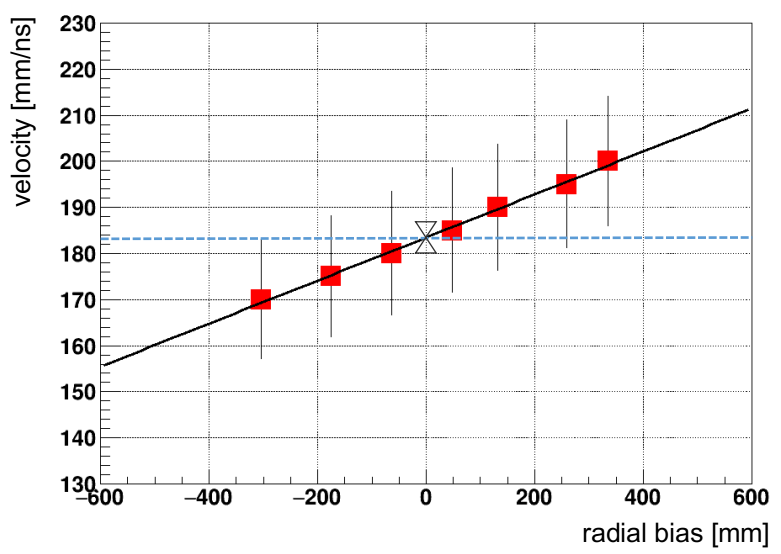
\includegraphics[width=6.5cm]{tune_groupVelocity_scint.png}
		\end{minipage}
	}   
	\subfigure[Tuning the $v_{gr,water}$.]{ 
		\begin{minipage}[t]{0.4\textwidth}
			\centering
			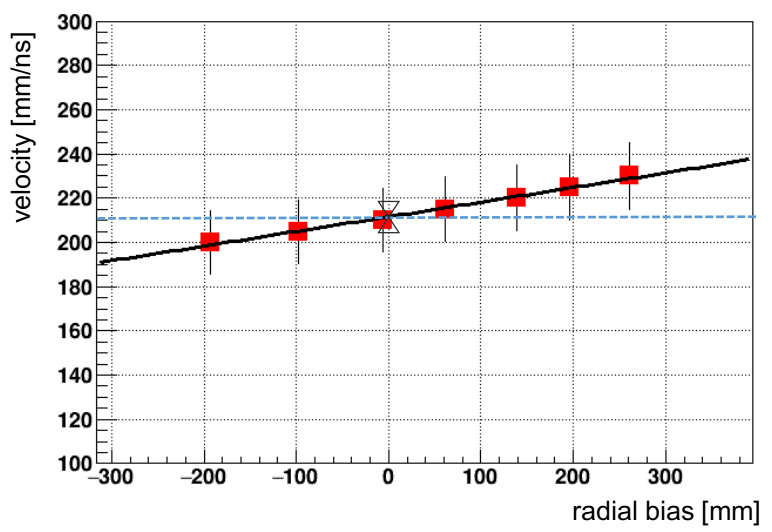
\includegraphics[width=6.5cm]{tune_groupVelocity_water.png}
		\end{minipage}
	}
\end{figure}

\begin{table}[ht]
	\centering
	\caption{\label{partial_groupV}Tuned effective group velocities for different PPO concentrations.}	
	{\centering
		\begin{tabular*}{140mm}{c@{\extracolsep{\fill}}ccccc}
			\toprule 
			PPO [g/L] & $V_{gr,scint}$ [mm/ns]& $n_{eff,scint}$ & $V_{gr,water}$ [mm/ns]& $n_{eff,water}$\\
			\midrule
			0.25 & 184.068$\pm$5.153 & 1.629 & 211.871$\pm$5.731 & 1.415\\
			0.5  & 183.467$\pm$5.159 &1.634& 211.587$\pm$-5.773 & 1.417 \\
			1.0 & 182.93$\pm$5.193 &1.639& 211.393$\pm$5.805& 1.418 \\
			2.0 & 183.045$\pm$5.184& 1.638& 211.629$\pm$5.767 & 1.417	\\
			6.0 & 184.218$\pm$5.135& 1.627& 211.173$\pm$5.843 &1.420\\
			\bottomrule	
		\end{tabular*}
	}
\end{table}

\subsection{Partial Fitter Performances}
The performance of the \texttt{MP partial fitter} was studied with MC simulations. During the partial-fill phase, the filling and mixing of the liquid scintillator was stable at several water levels for data taking and data analysis. A typical water level is at 3 m in the AV coordination and a typical PPO concentration is 0.5 g/L. With these two settings in the partial-fill geometry, 5000 3-MeV $e^-$ were simulated inside the scintillator region and the water region respectively to test the partial fitter performances.

The average fit speed of the vertex reconstruction of the events in the scintillator region is 0.2 second/event, which is acceptable for the data processing during the partial-fill phase. For the events in the water region, the average fit speed is 0.05 s/event, which is similar to the \texttt{MPW fitter}. Fig.~\ref{fig:partial_inScint} and Fig.~\ref{fig:partial_inWater} show the results of the \texttt{MP partial fitter} reconstructed positions in the scintillator and water regions respectively. The subfigure (a) is the reconstructed positions projected on $\rho=\sqrt{x^2+y^2}$ and $z$ while the subfigures (b), (c) and (d) are the position biases between the reconstruction and MC. The distributions of position biases are fit with Gaussian functions and the values of Gaussian mean ($\mu_{x,y,z}$) and sigma ($\sigma_{x,y,z}$) to quantify the fit biases and resolutions. 

\begin{figure}%[htbp]
	\centering
	\subfigure[$\rho=\sqrt{x_{fit}^2+y_{fit}^2}$ vs. $z_{fit}$.]
	{ 
		\begin{minipage}[b]{0.38\textwidth}
			\centering
			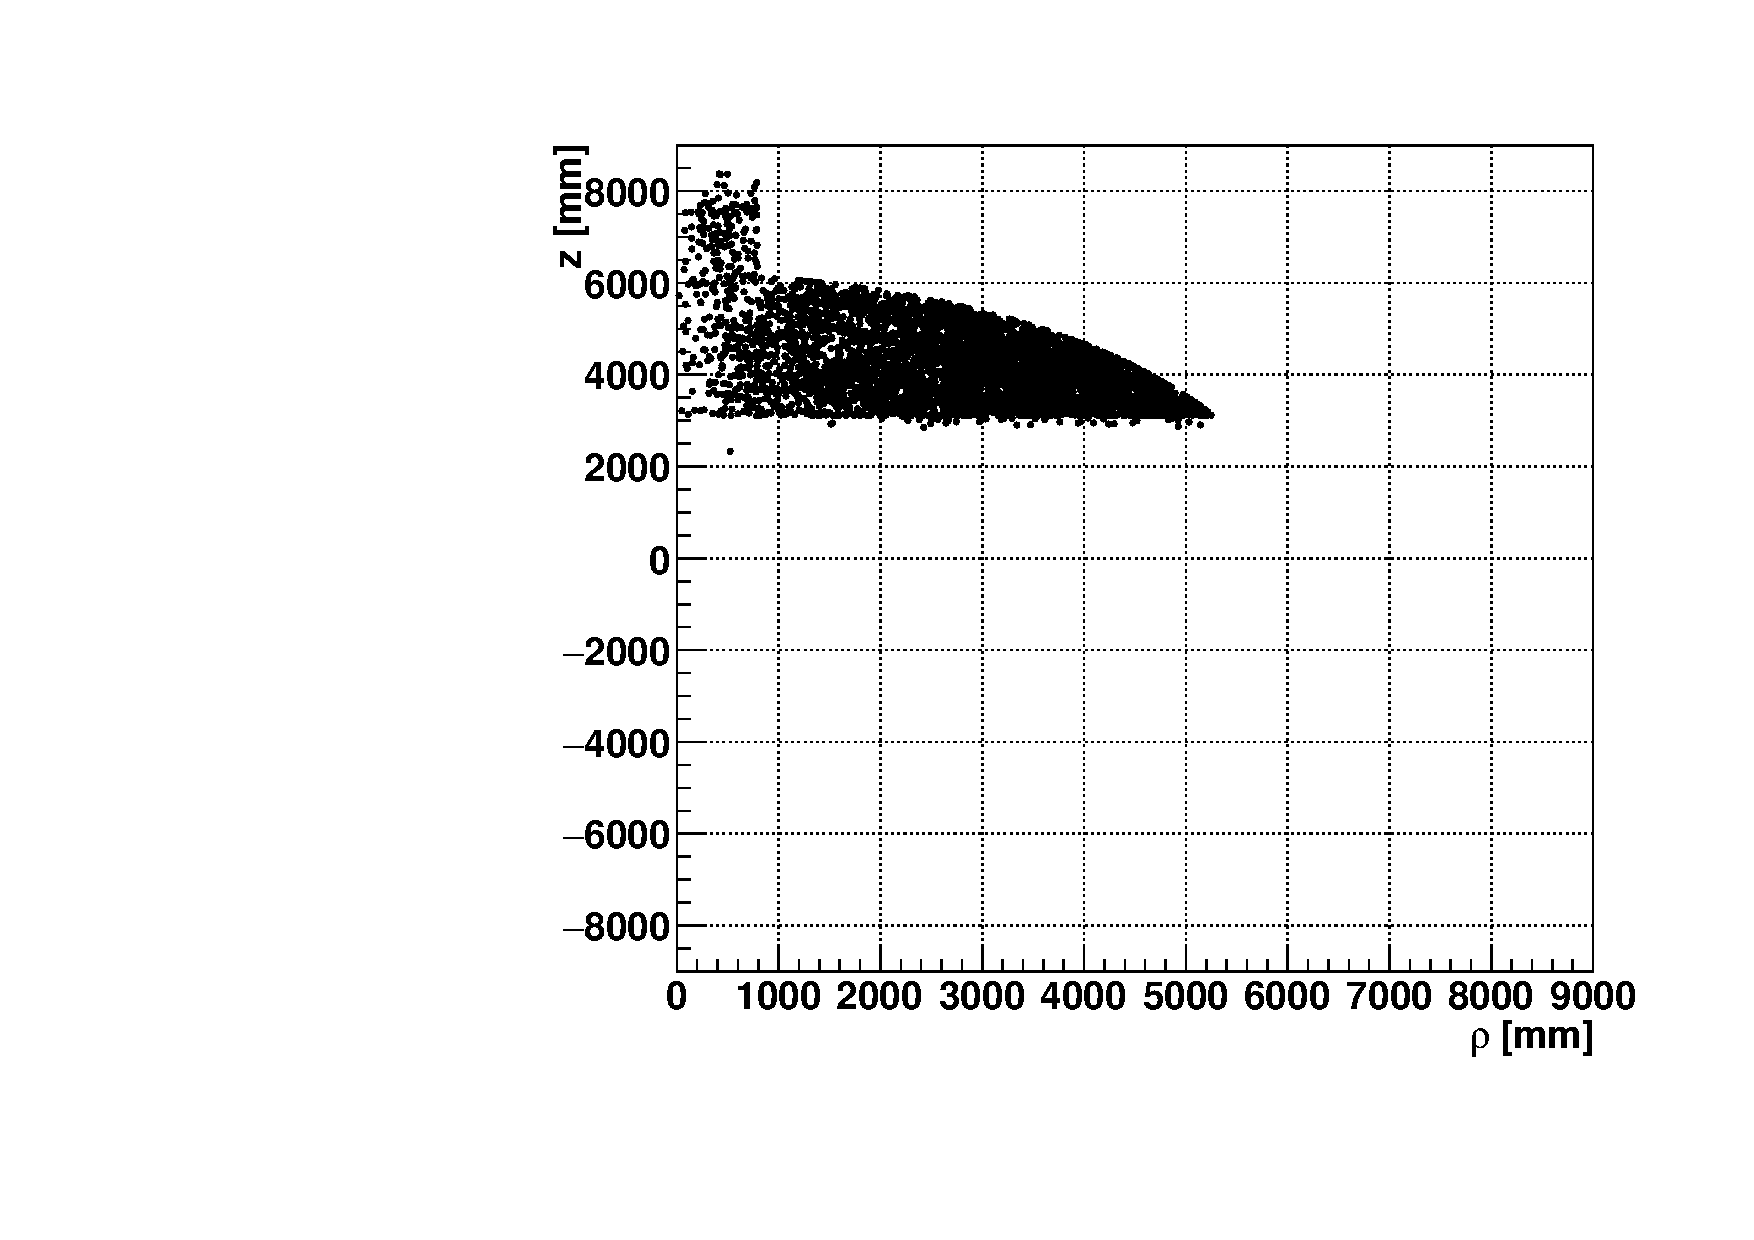
\includegraphics[width=6.5cm]{partial_top_3MeV_rhoVsZ.pdf}
		\end{minipage}
	}
	\subfigure[$x_{fit}-x_{mc}$.]{
		\begin{minipage}[t]{0.38\textwidth}
			\centering
			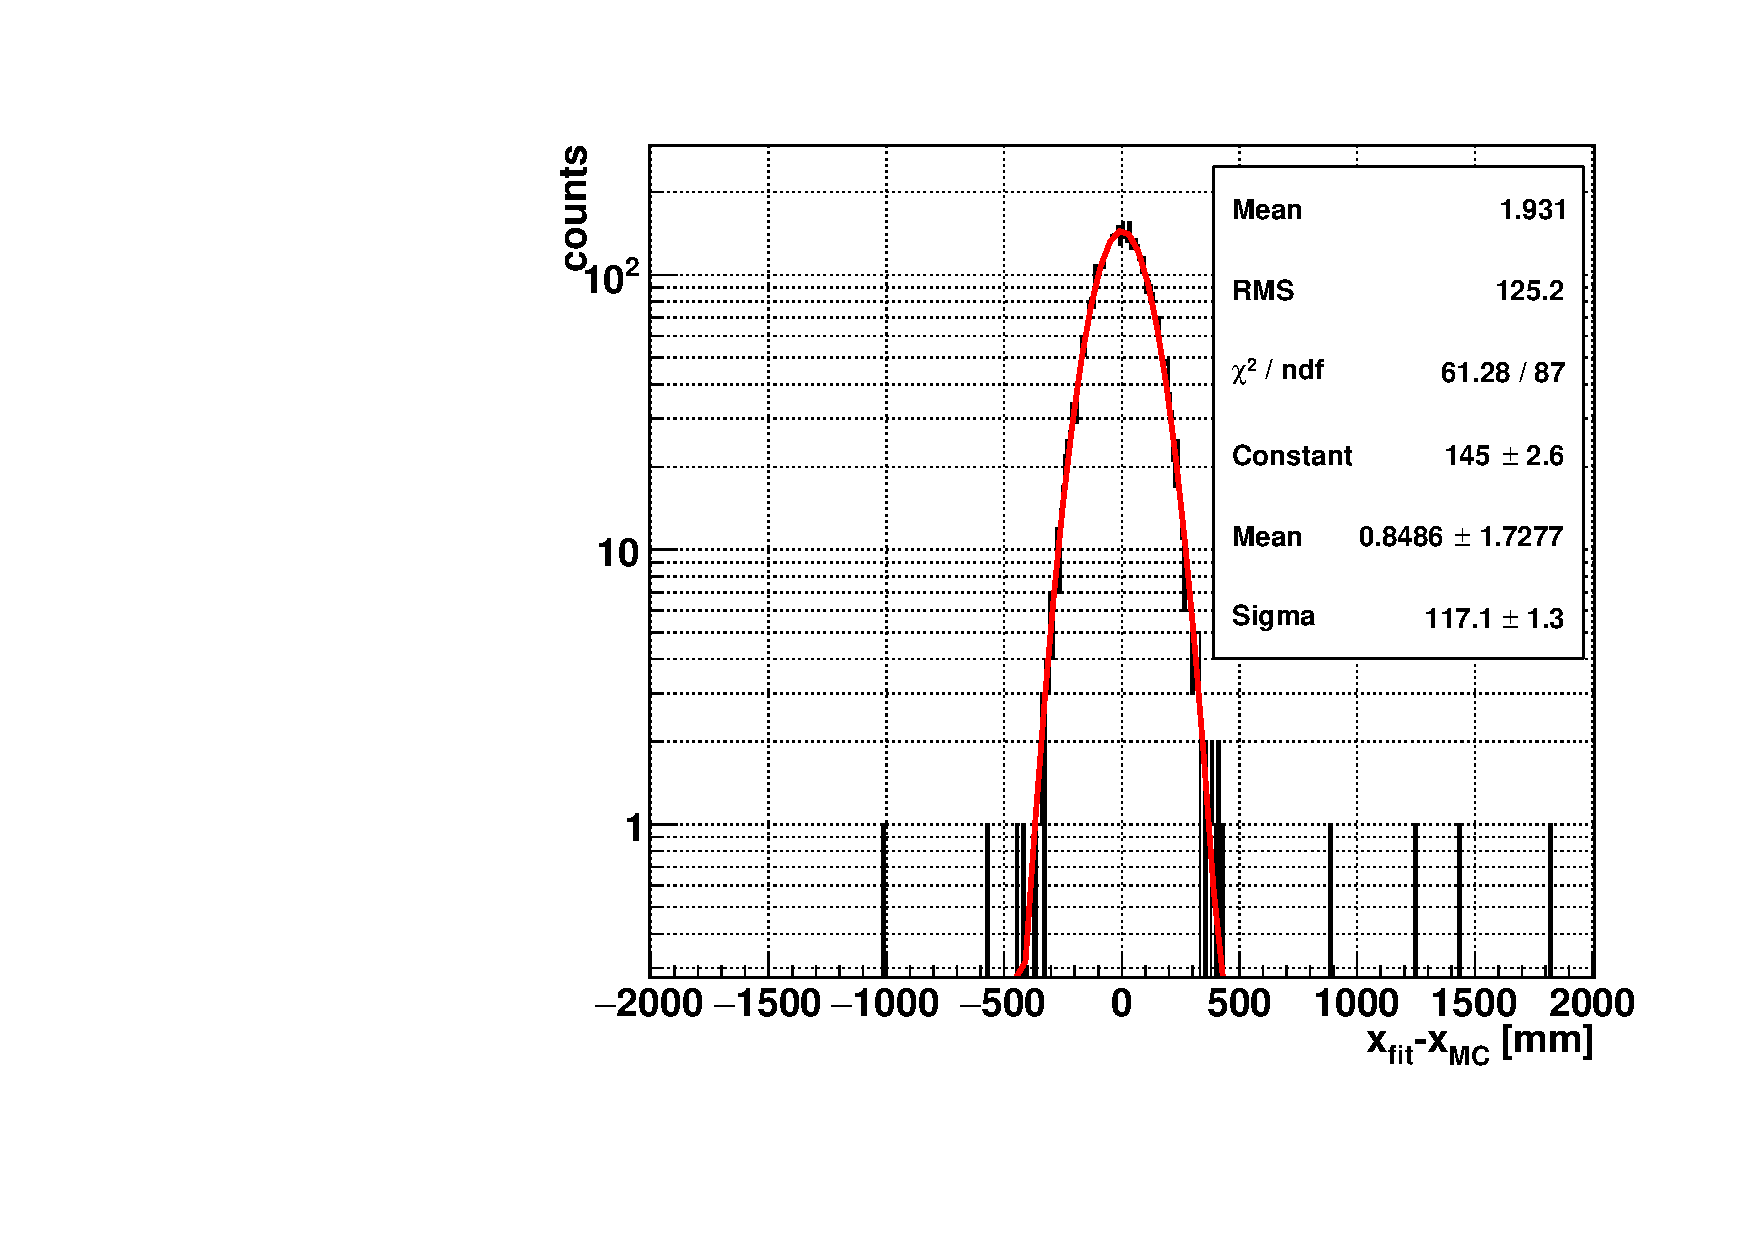
\includegraphics[width=6.5cm]{partial_top_3MeV_xbias.pdf}
		\end{minipage}
	}   
	\subfigure[$y_{fit}-y_{mc}$.]{
		\begin{minipage}[t]{0.38\textwidth}
			\centering
			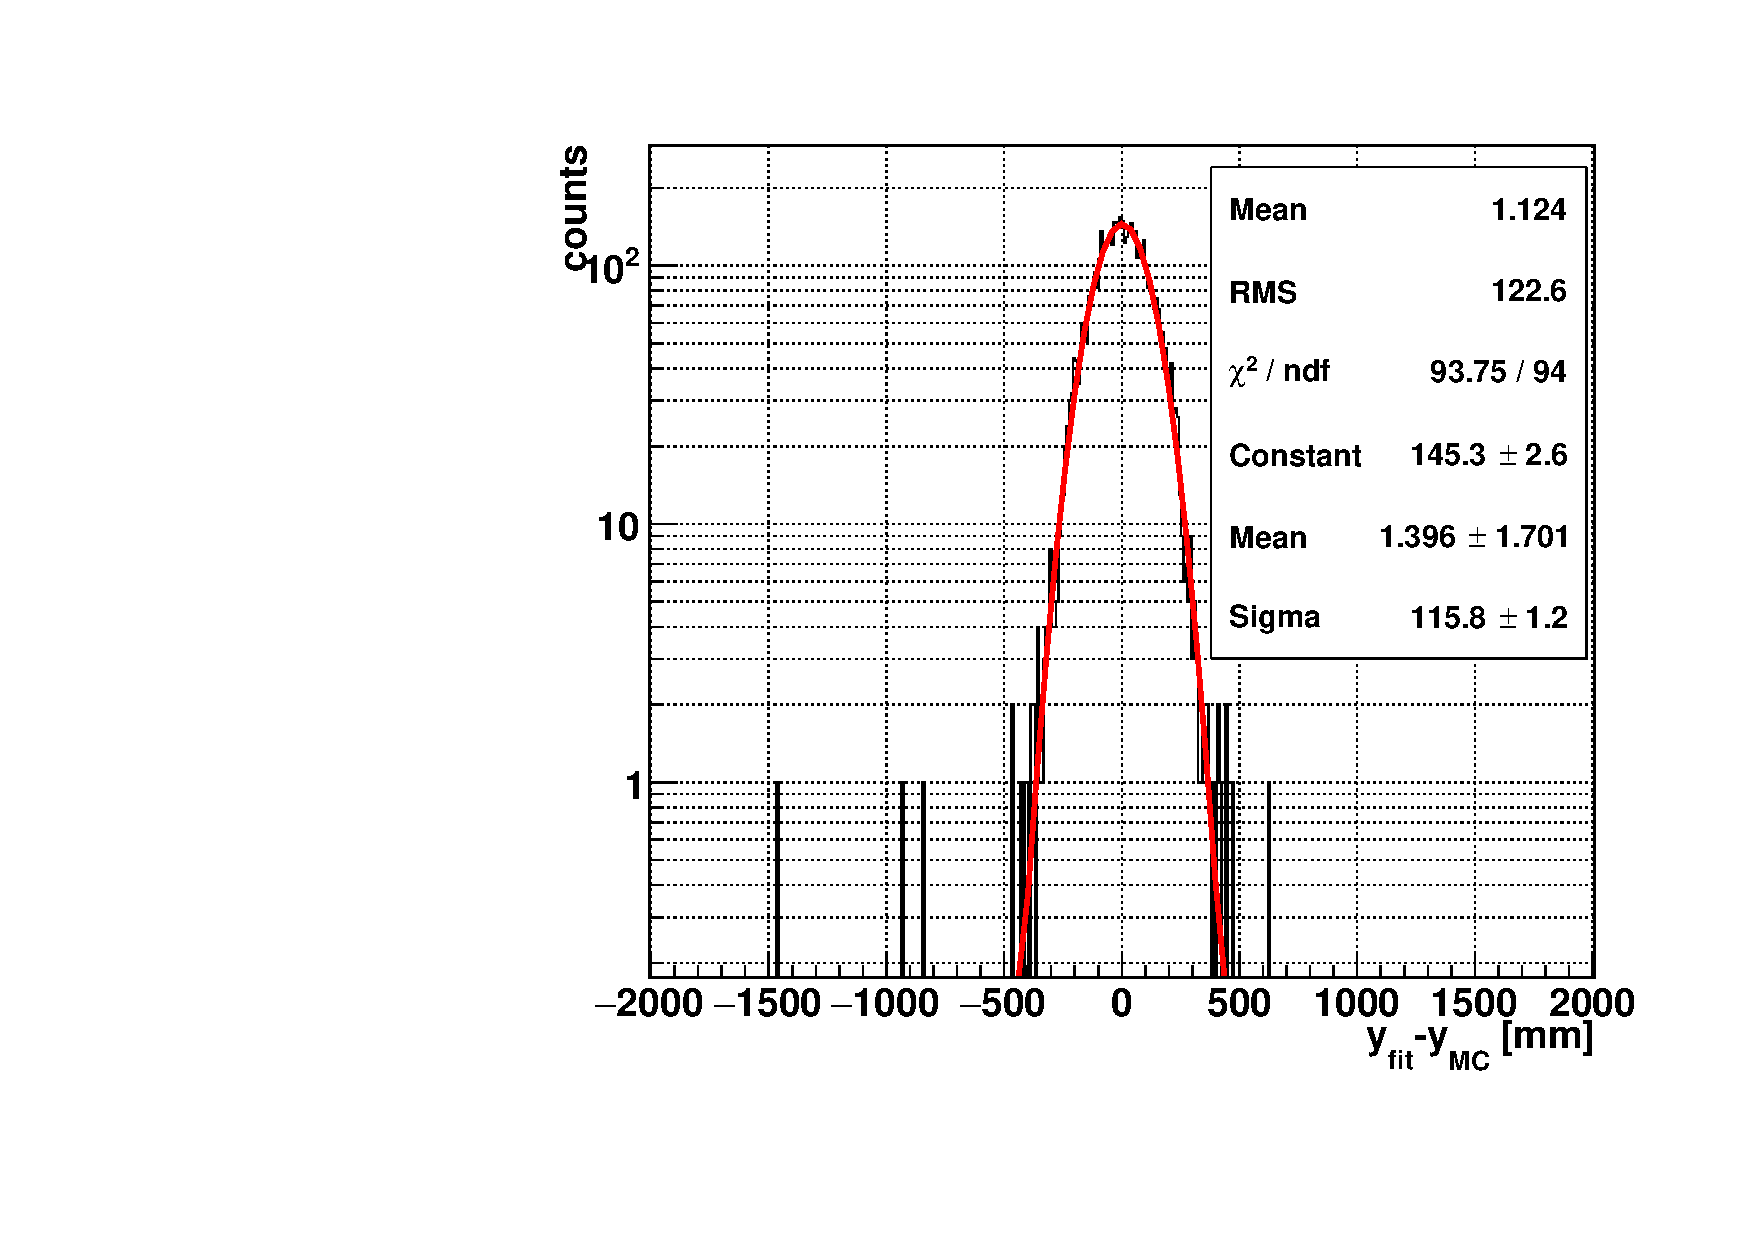
\includegraphics[width=6.5cm]{partial_top_3MeV_ybias.pdf}
		\end{minipage}
	}
	\subfigure[$z_{fit}-z_{mc}$.]{
		\begin{minipage}[b]{0.38\textwidth}
			\centering
			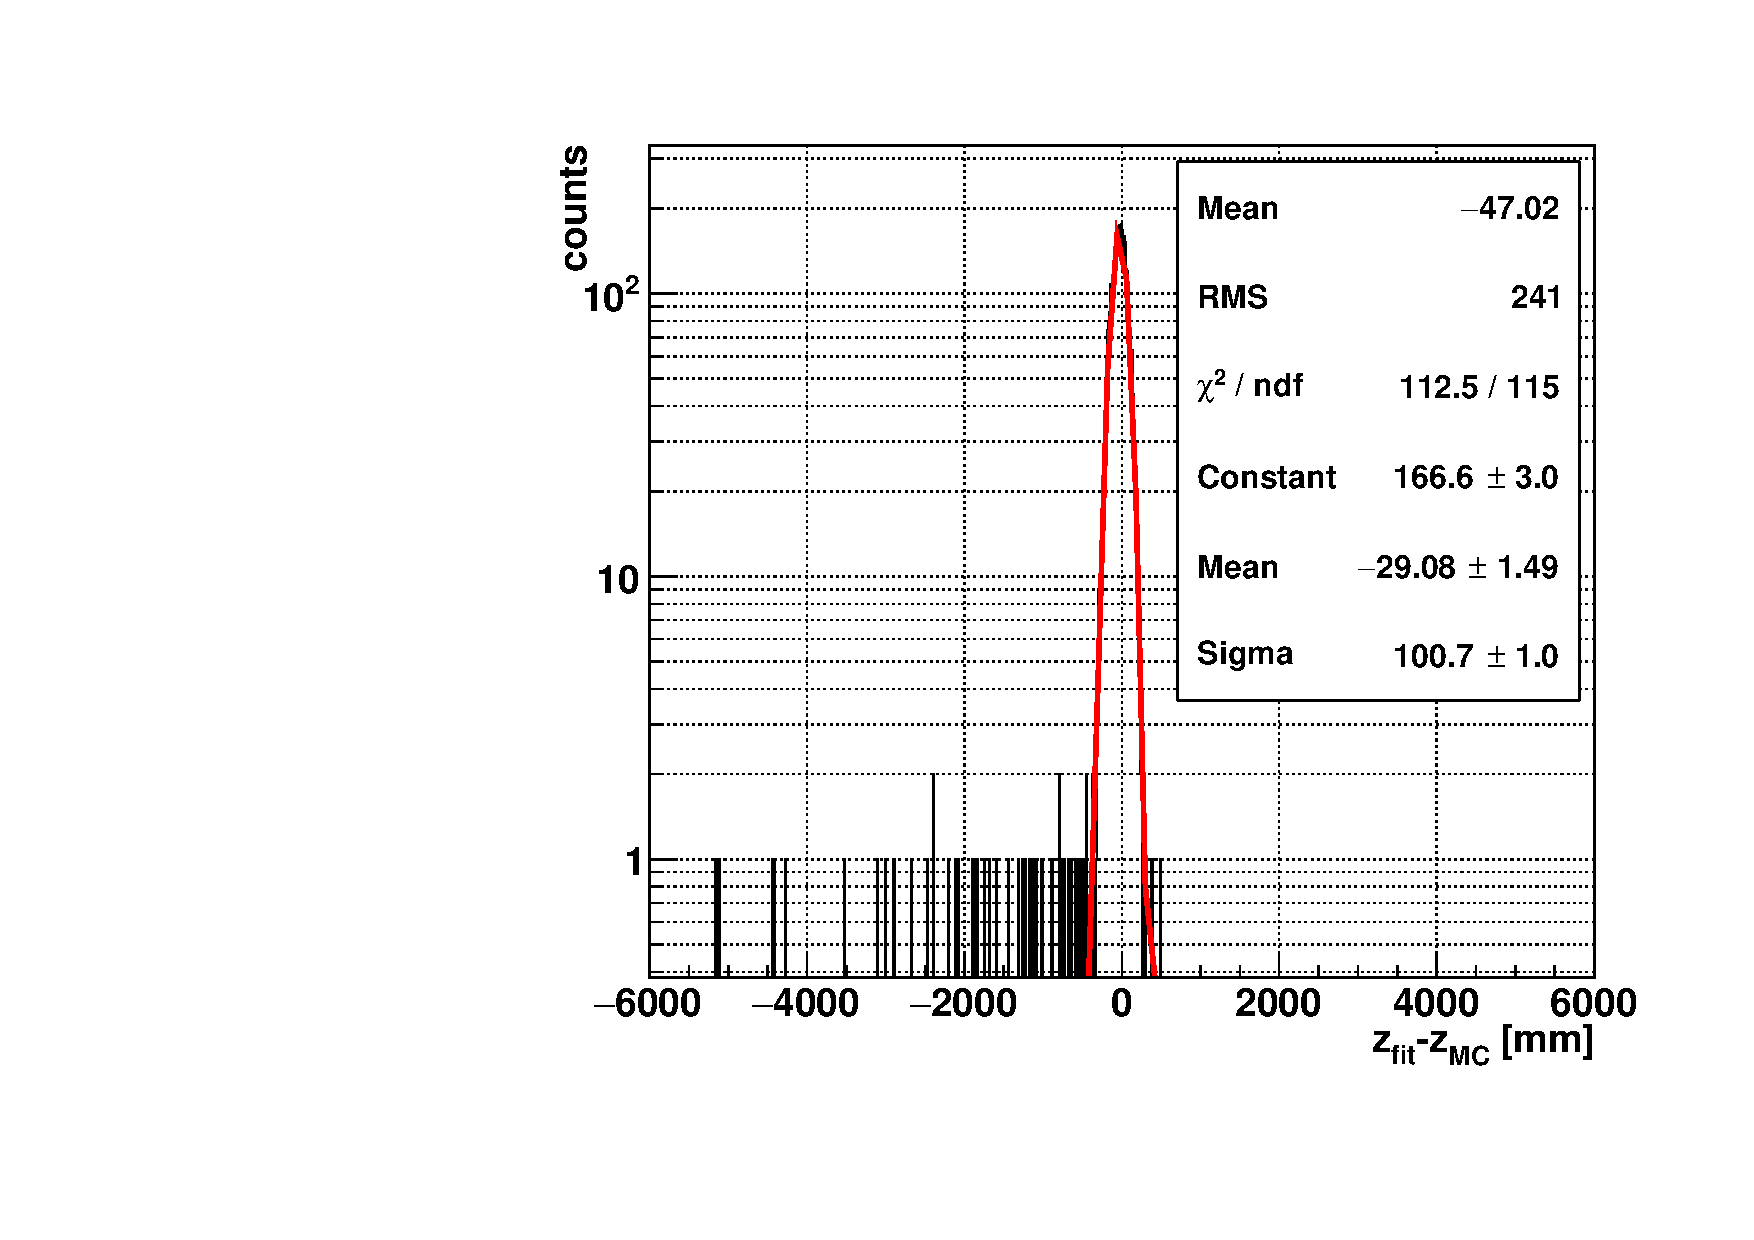
\includegraphics[width=6.5cm]{partial_top_3MeV_zbias.pdf}
		\end{minipage}
	}
	\caption{Reconstructed positions and fit biases of the 3-MeV $e^-$ events in the scintillator region.\label{fig:partial_inScint}}
\end{figure}

\begin{figure}%[htbp]
	\centering
	\subfigure[$\rho=\sqrt{x_{fit}^2+y_{fit}^2}$ vs. $z_{fit}$.]
	{ 
		\begin{minipage}[b]{0.38\textwidth}
			\centering
			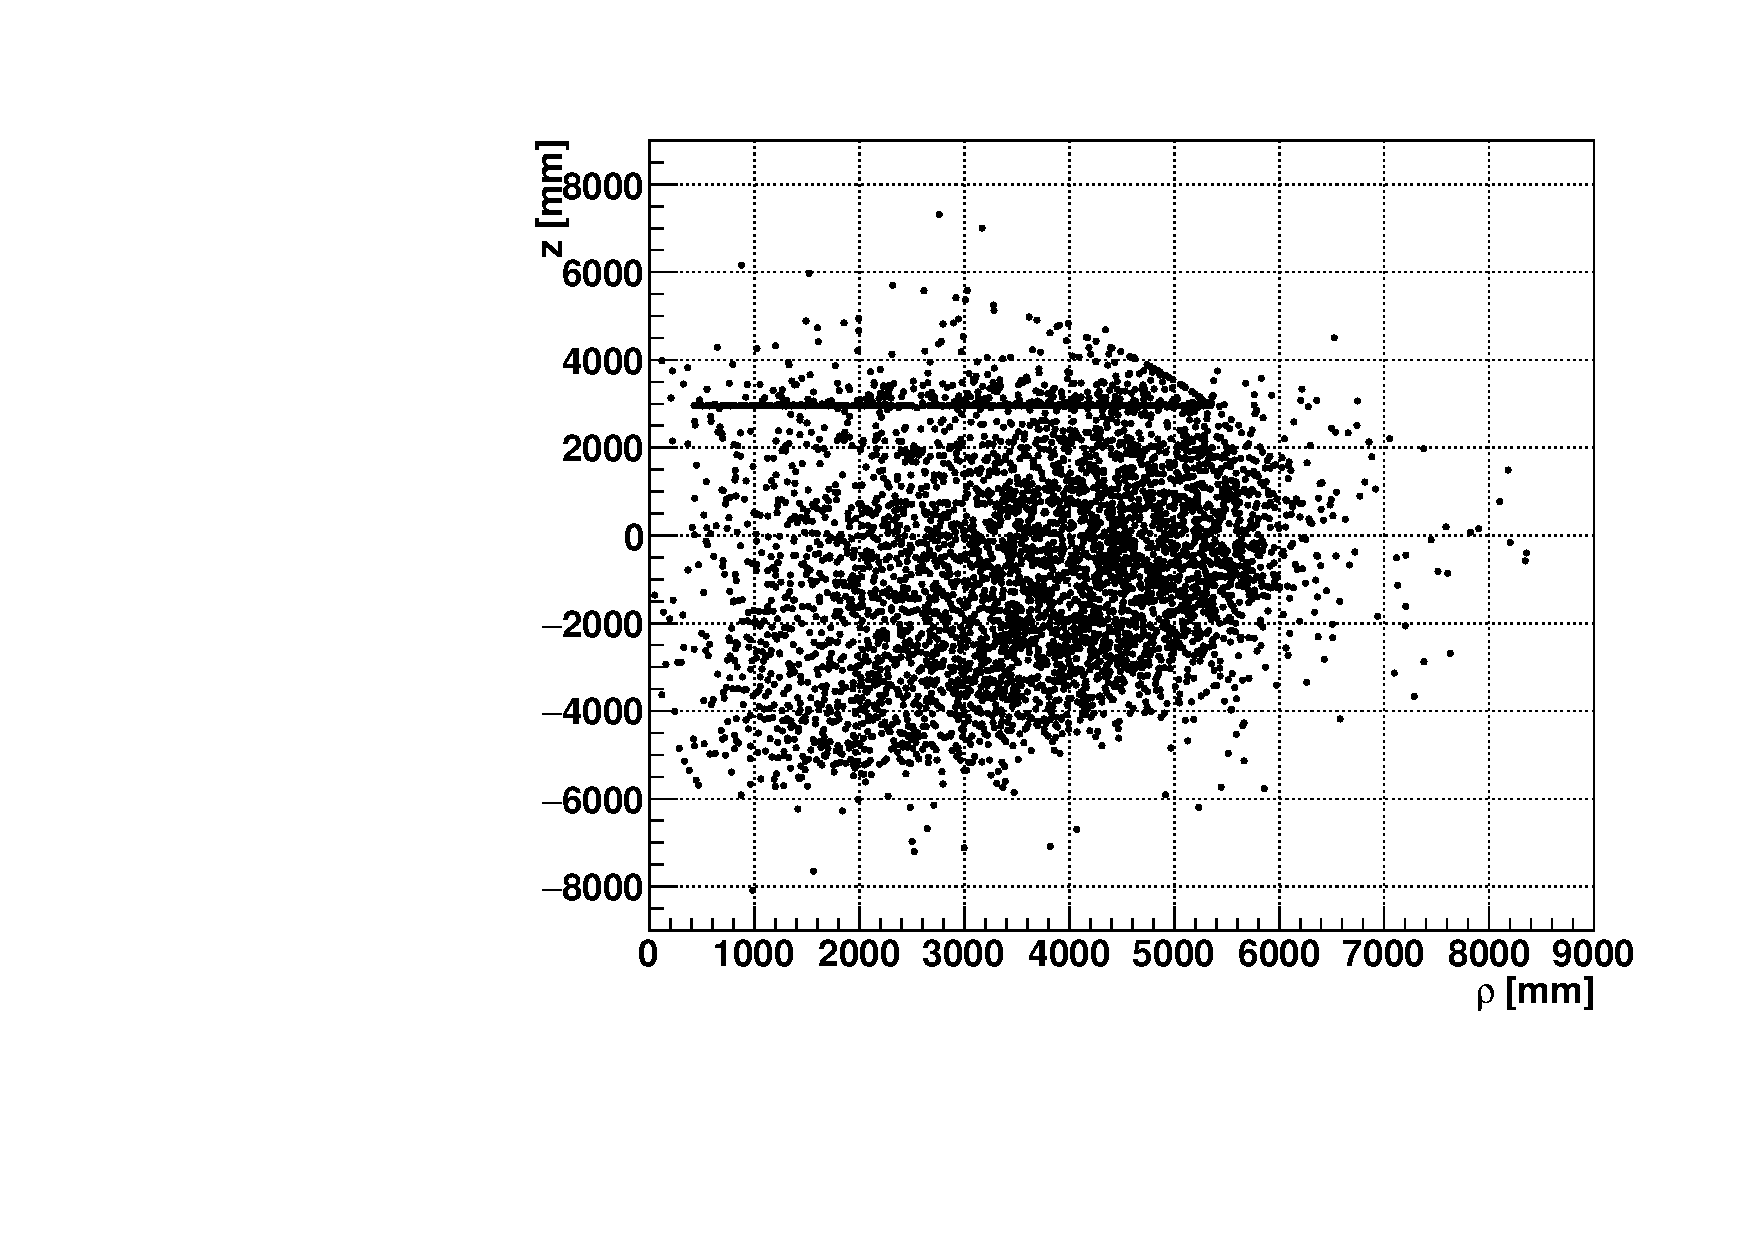
\includegraphics[width=6.5cm]{partial_bot_3MeV_rhoVsZ.pdf}
		\end{minipage}
	}
	\subfigure[$x_{fit}-x_{mc}$.]{
		\begin{minipage}[t]{0.38\textwidth}
			\centering
			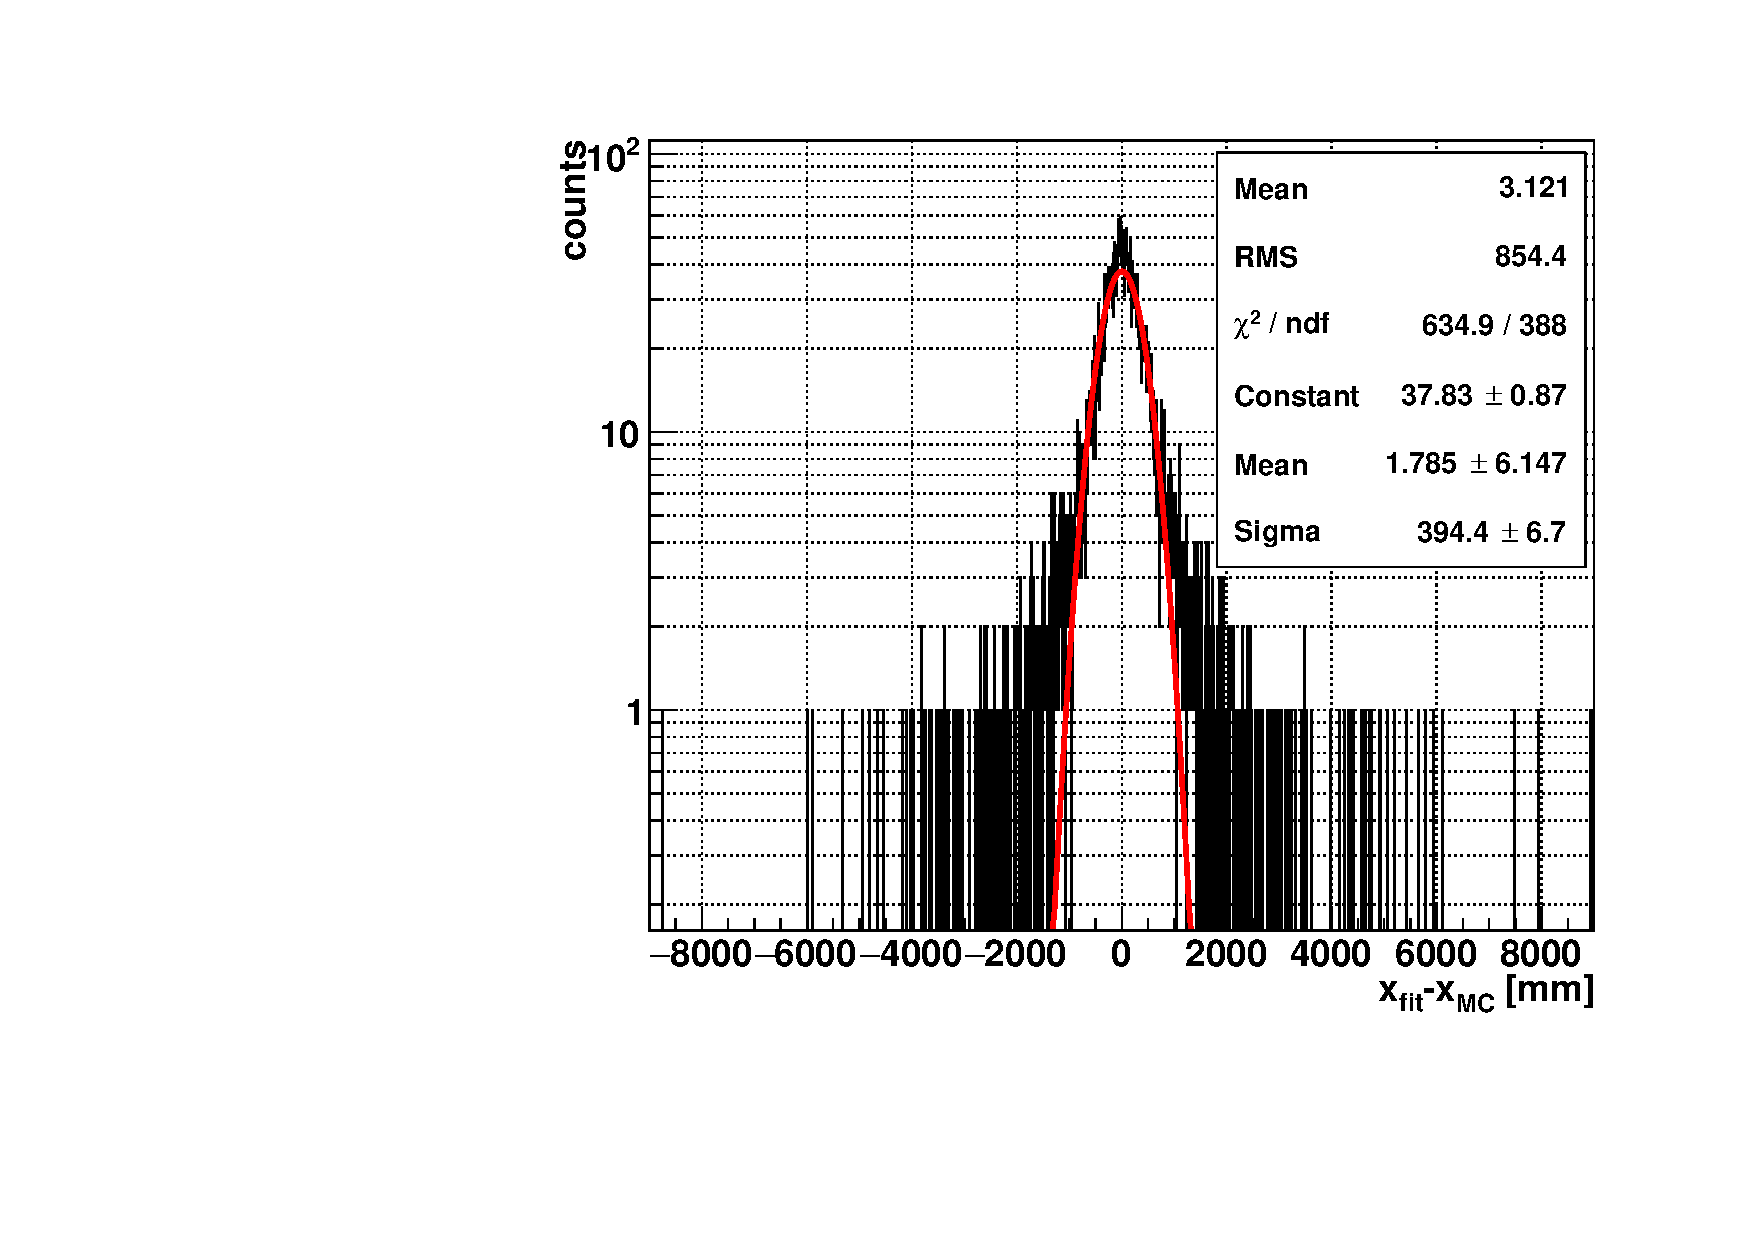
\includegraphics[width=6.5cm]{partial_bot_3MeV_xbias.pdf}
		\end{minipage}
	}   
	\subfigure[$y_{fit}-y_{mc}$.]{ 
		\begin{minipage}[t]{0.38\textwidth}
			\centering
			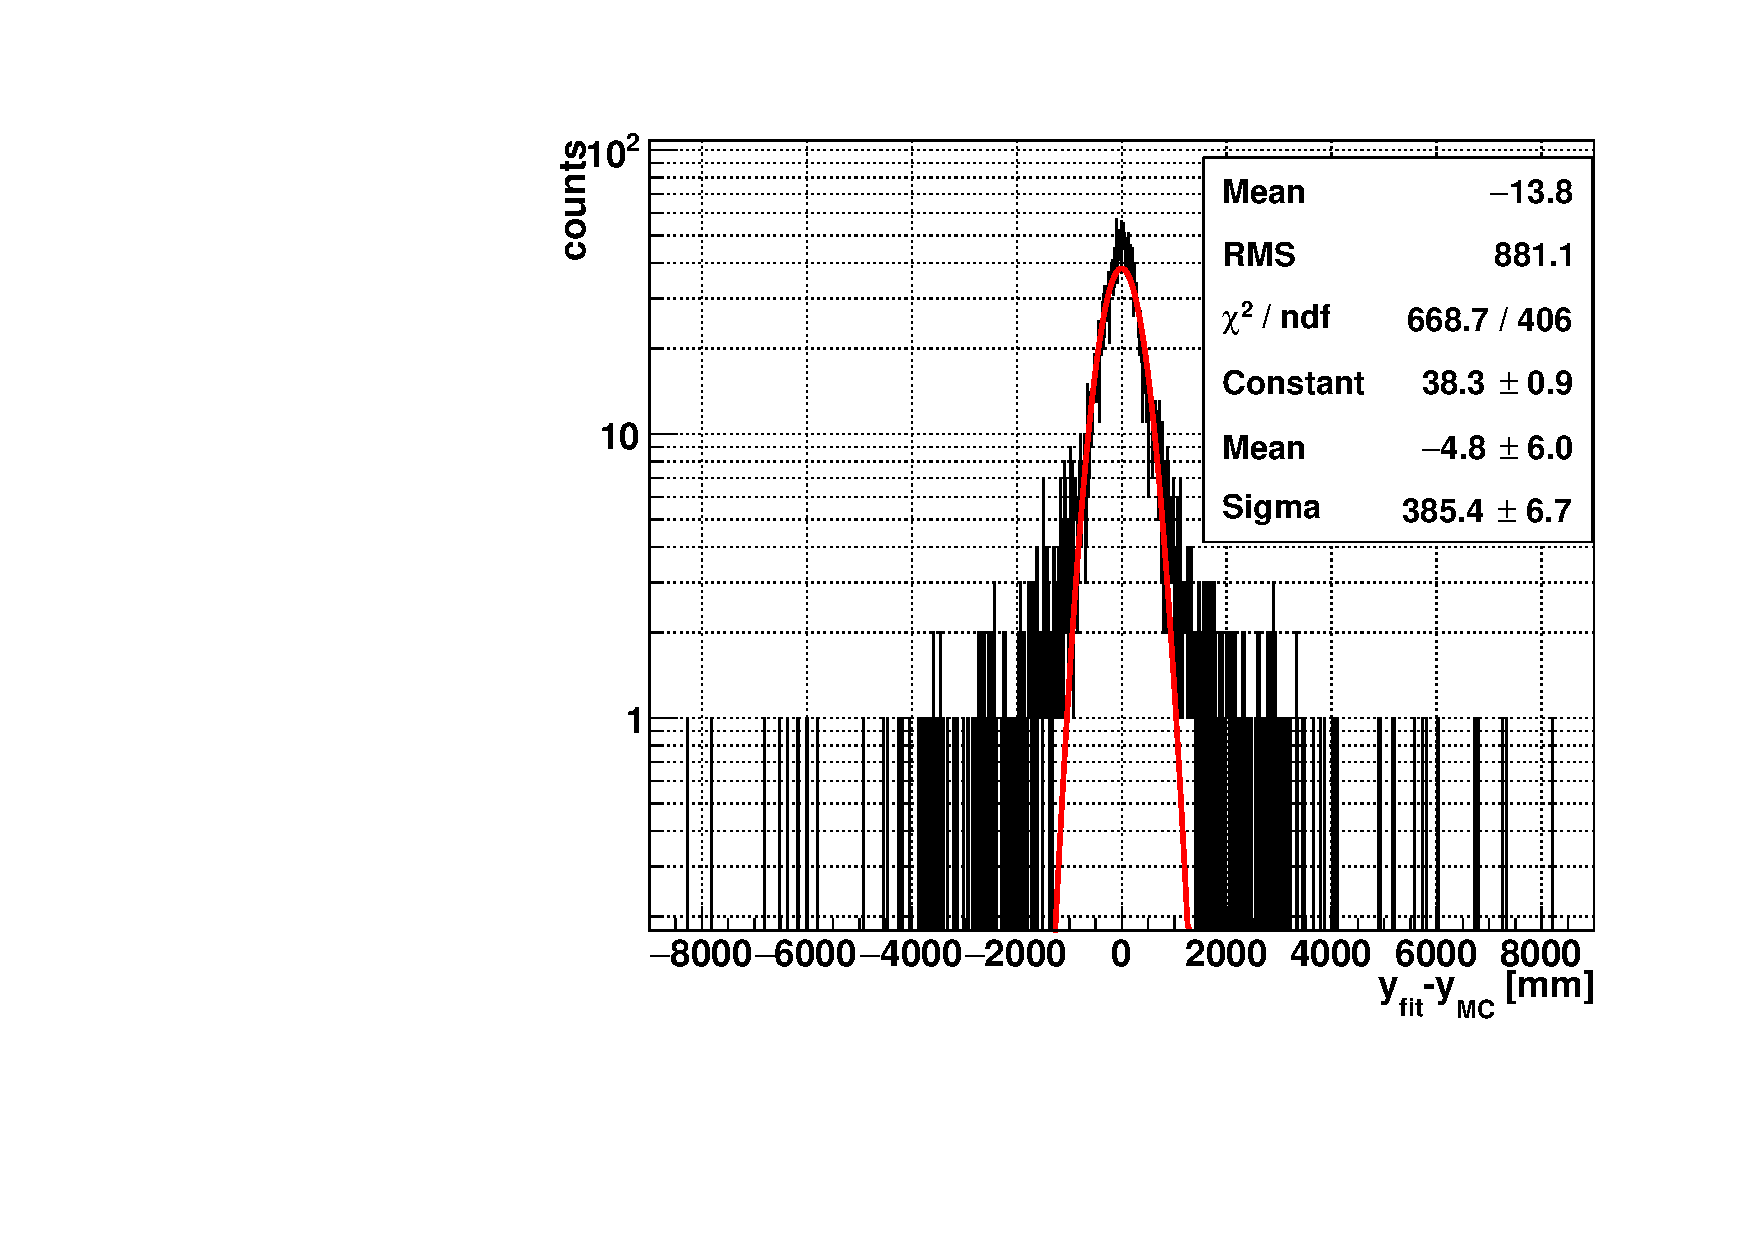
\includegraphics[width=6.5cm]{partial_bot_3MeV_ybias.pdf}
		\end{minipage}
	}
	\subfigure[$z_{fit}-z_{mc}$.]{ 
		\begin{minipage}[b]{0.38\textwidth}
			\centering
			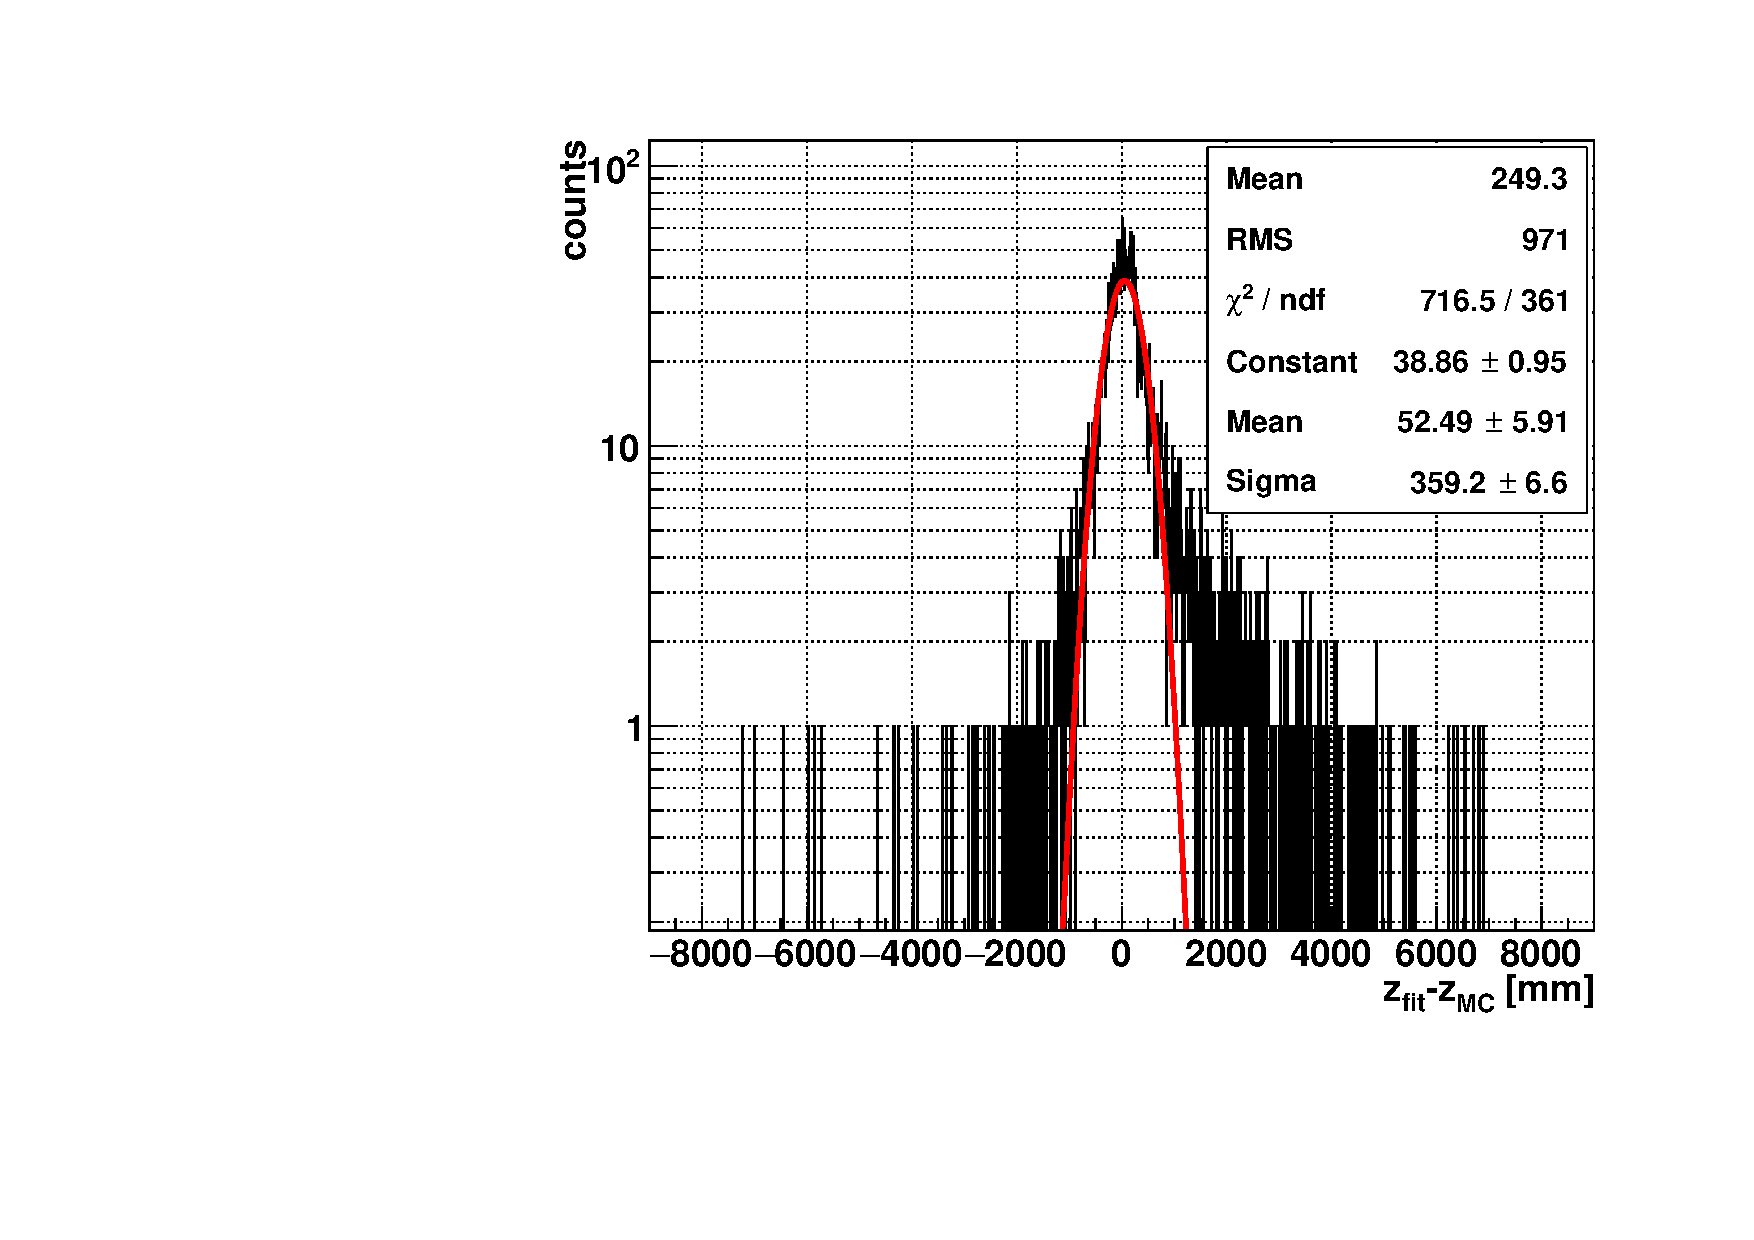
\includegraphics[width=6.5cm]{partial_bot_3MeV_zbias.pdf}
		\end{minipage}
	}
	\caption{Reconstructed positions and fit biases of the 3-MeV $e^-$ events in the water region.\label{fig:partial_inWater}}
\end{figure}


It shows that, for the events in the scintillator region, the resolutions $\mu_{x,y,z}$ reach about 150 mm and the biases are within 2 mm in the x and y axes while there are about -50 mm biases in the z axes. The offset in z 
mis-reconstruction

For the events in the water region, the fit position biases in x and y are comparable to the results of the \texttt{MPW fitter} shown in Sect.~\ref{sect:waterFitterVertex}, while the bias in z is about 50 mm worse and the resolutions are about 100 mm worse. This is due to the effects from the water-scintillator interface and boundaries, which makes to fitter to push the events to the boundaries and thus causes the mis-reconstructions of the fitter. These boundary effects can be seen in the $\rho$ vs. $z$ plot in the subfigure (d). However, the interested events for the partial-fill analysis are always the events in the scintillator and cuts on NHits are applied on the partial-fill data to remove the water events. 

For the $posFoM$ cut, applying a $scaleLogL>9.8$ cut can remove about 38\% of the mis-reconstructed events with $|\vec{X}_{fit}-\vec{X}_{MC}|>1000$ mm.
As shown in Fig.~\ref{fig:partial_scaleLogLcut} (c), this cut removes most of the outliers in $\rho-z$ plot compared to the Fig.~\ref{fig:partial_scint_a}

\begin{figure}[htbp]
	\centering
	\subfigure[$z_{fit}-z_{MC}$ vs. $scaleLogL$.]{ 
		\begin{minipage}[b]{0.38\textwidth}
			\centering
			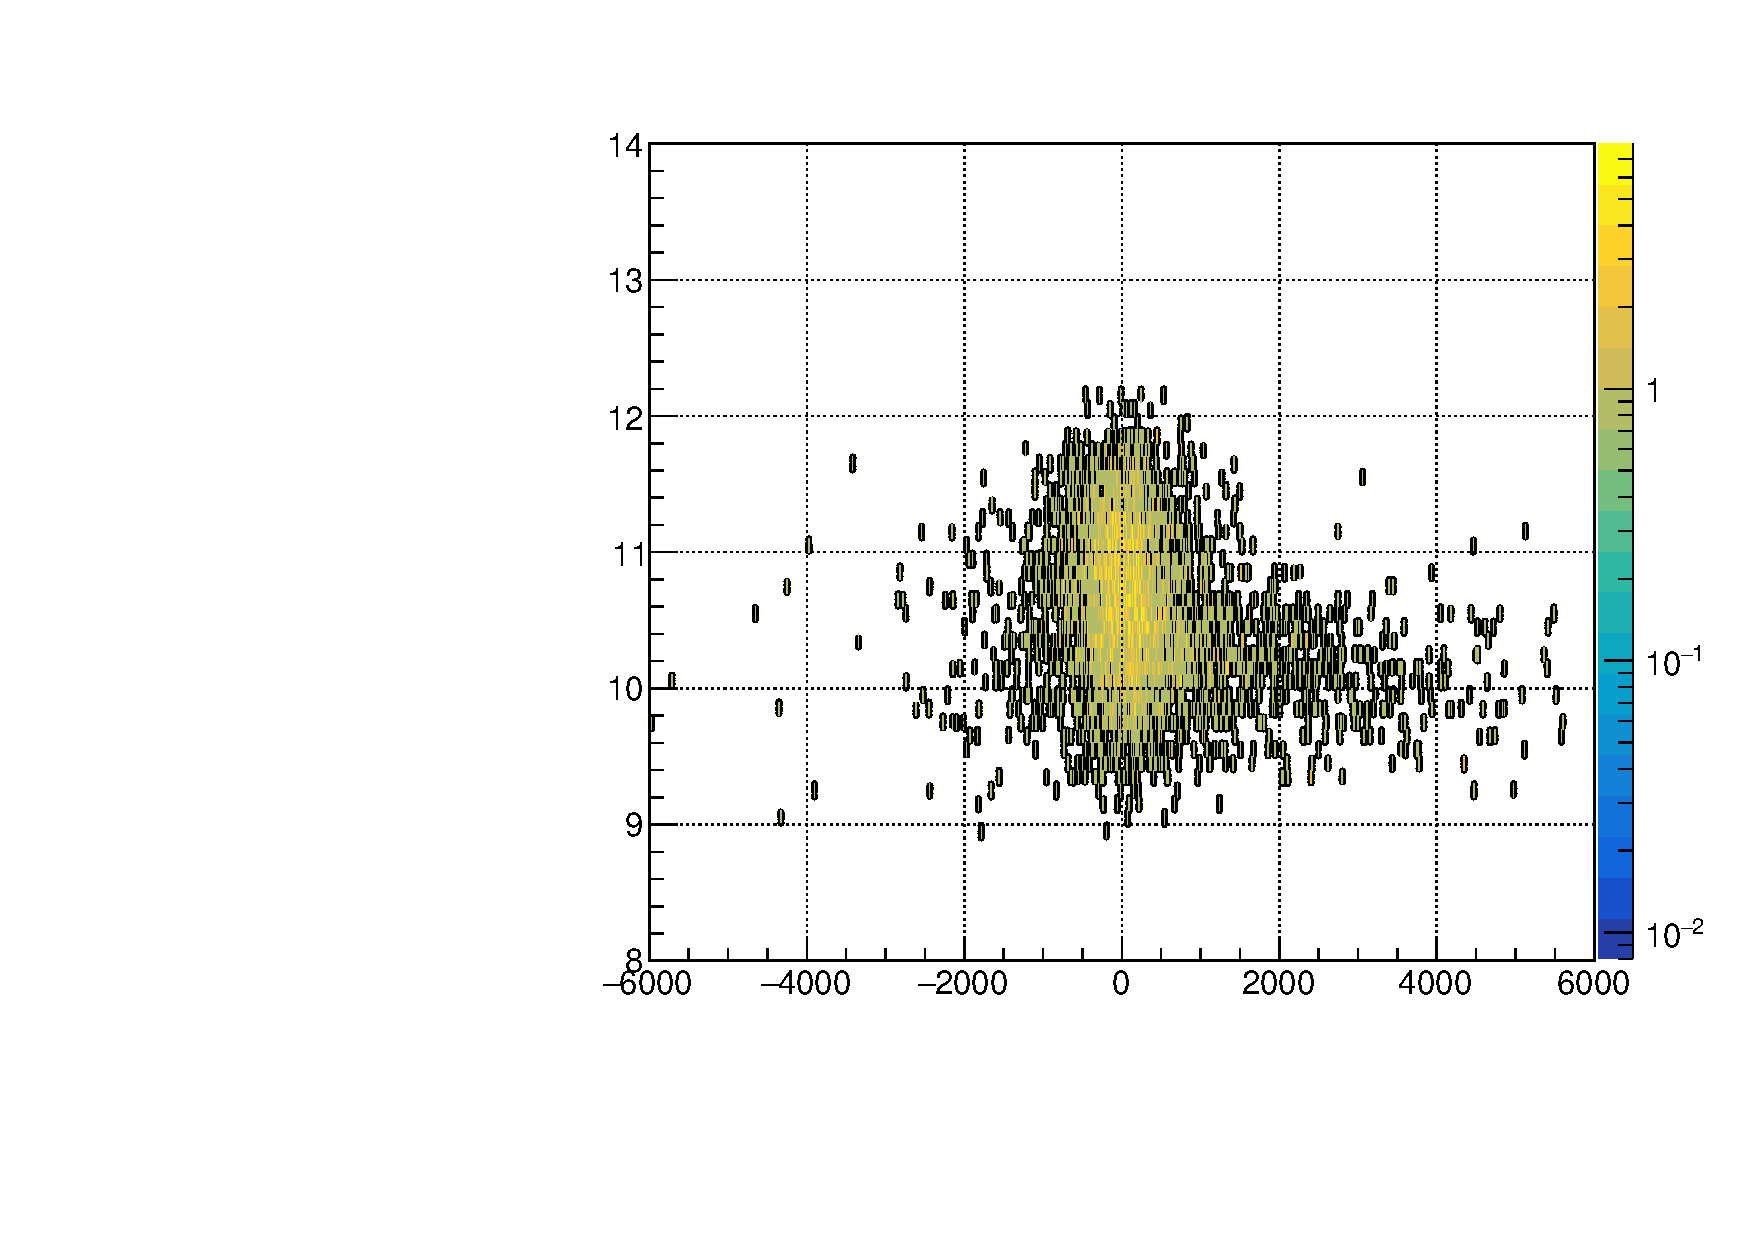
\includegraphics[width=6.5cm]{scaleLogLvsZbias_bot.pdf}
		\end{minipage}
	}
	\subfigure[$x_{fit}-x_{mc}$.]{
		\begin{minipage}[t]{0.38\textwidth}
			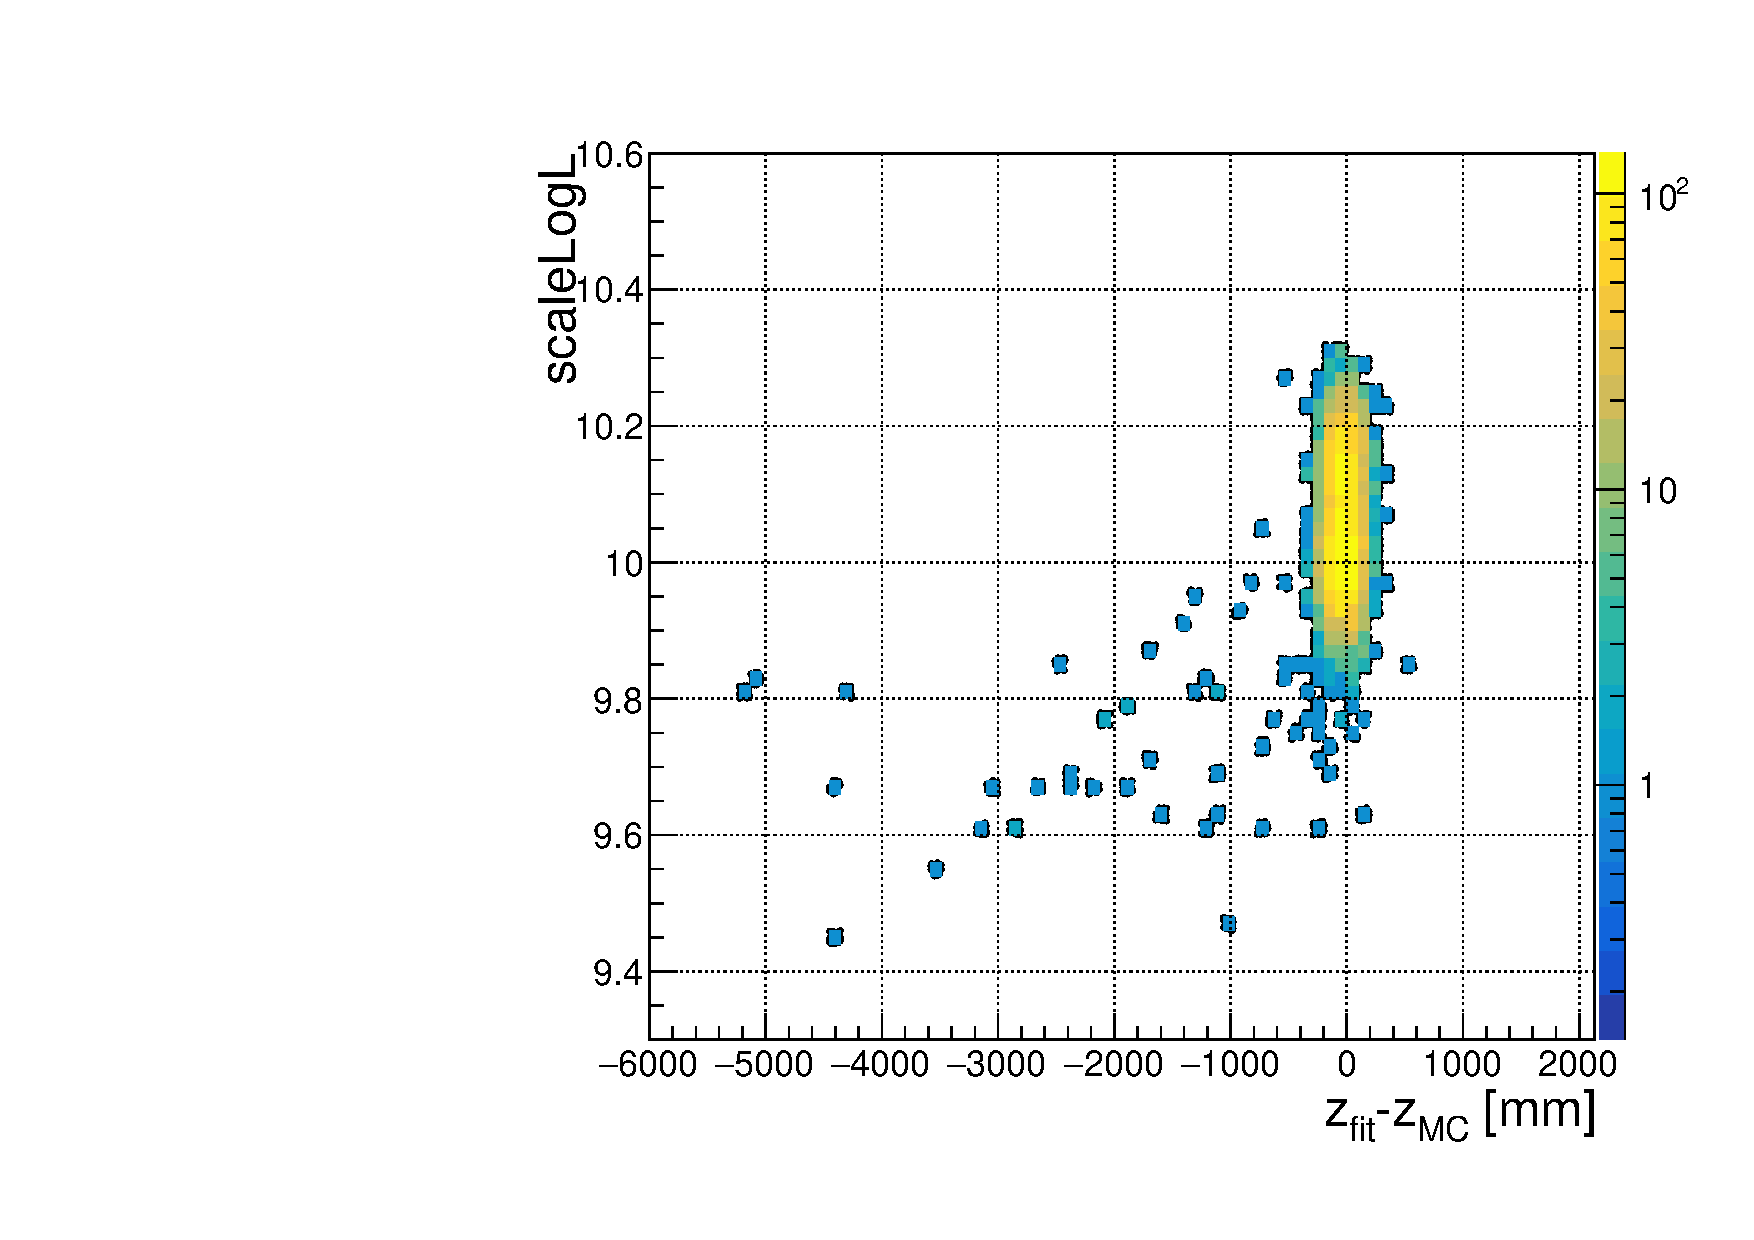
\includegraphics[width=6.5cm]{scaleLogLvsZbias_top.pdf}
		\end{minipage}
	}   
	\subfigure[$\rho_{fit}$ vs. $z_{fit}$.]{ 
		\begin{minipage}[t]{0.38\textwidth}
			\centering
			\includegraphics[width=6.5cm]{scaleLogLvsZbias_top_scaleLogL9p8.pdf}
		\end{minipage}
	}
	\caption{Reconstructed positions and fit biases after applying the posFoM cuts.\label{fig:partial_scaleLogLcut}}
\end{figure}

A discussion for improving the fitter will be shown in Sect.\ref{sect:partialFitterDiscuss}.

\subsubsection{Test on Different PPO Concentrations}
To study the effects of different PPO concentrations, in the partial-fill geometry, the water level was set at 3 m, and the PPO concentrations were set to 0.25, 0.5, 1, 2, and 6 g/L respectively. Simulations of 5000 3-MeV $e^-$ were generated in the scintillator region with uniformly distributed positions and isotropic directions. The \texttt{MP partial fitter} uses the effective velocities and $PDF$s re-coordinated to the simulation geometries with corresponding PPO concentrations. The distributions of the position biases between the reconstruction and MC in x, y, and z axes were fitted with Gaussians to obtain the fit position biases ($\mu_{x,y,z}$) and resolutions ($\sigma_{x,y,z}$).

Fig.~\ref{fig:partialBiasVsPPO} and Fig.~\ref{fig:partialResolVsPPO} show the $\mu_{x,y,z}$ and $\sigma_{x,y,z}$ against PPO concentrations. It shows that the values of $\mu_{x,y,z}$ are stable in the [-15,15] mm region, while the values of $\sigma_{x,y,z}$ decrease from about 150 mm to about 60 mm as the concentration increases. The light yield of the liquid scintillator goes up as the PPO concentration increases, which gives larger NHits and more PMT information for the fitter. However, the differences between the 2 g/L and 6 g/L cases are small, which indicates a saturation effect for the PPO concentration above 2 g/L.

\begin{figure}[!htb]
	\centering
	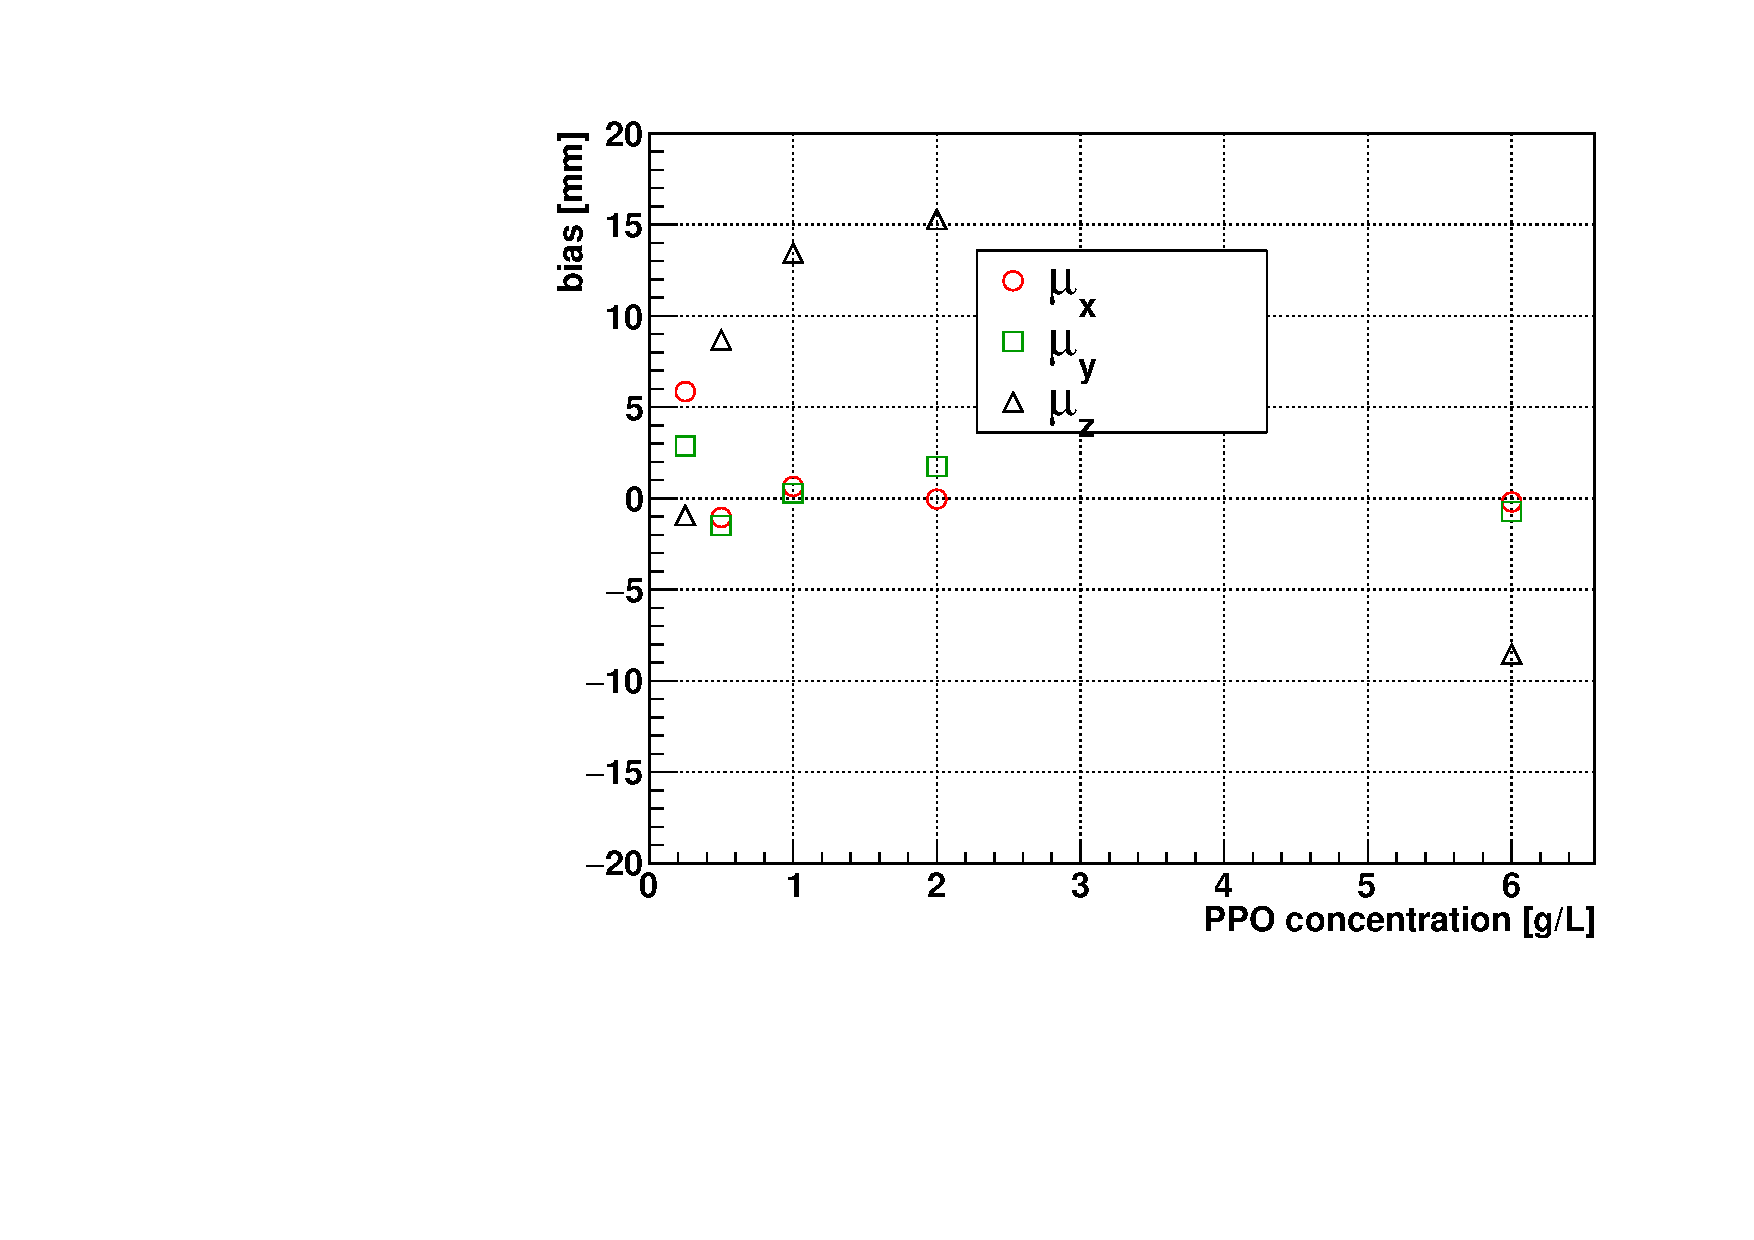
\includegraphics[width=10cm]{partialBiasVsPPO.pdf}
	\caption{Fit position biases against the PPO concentrations.}
	\label{fig:partialBiasVsPPO}
\end{figure}

\begin{figure}[!htb]
	\centering
	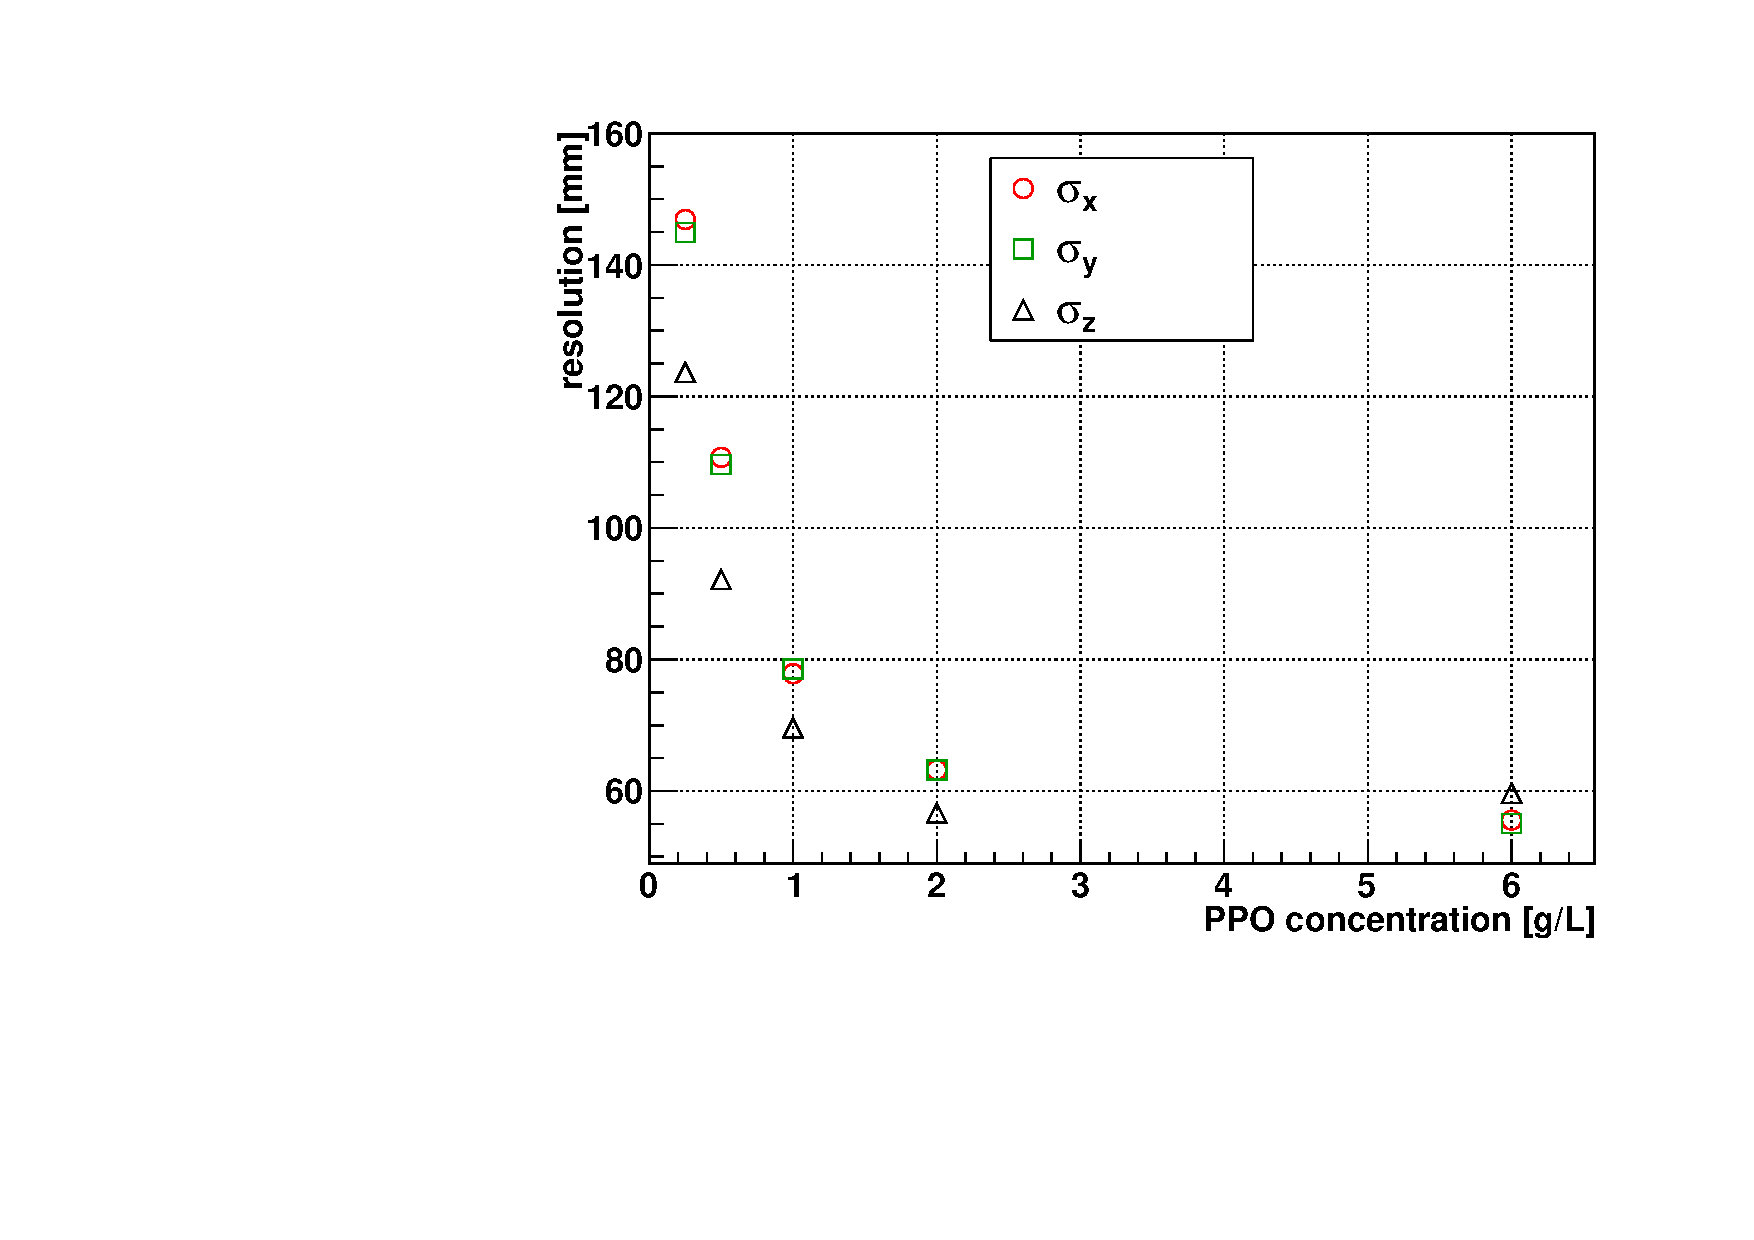
\includegraphics[width=10cm]{partialResolVsPPO.pdf}
	\caption{Fit position resolutions against the PPO concentrations.}
	\label{fig:partialResolVsPPO}
\end{figure}

If using a timing $PDF$ with the wrong PPO concentration for the reconstruction, the effect on reconstruction is small\cite{partialFitterPDFtestInvulnerable}. I simulated 3-MeV $e^-$ uniformly distributed in the LAB+0.25 g/L PPO scintillator with isotropic directions, and then reconstructed the events by using the timing $PDF$ of 0.5, 1 and 2 g/L PPO (higher concentrations) respectively. All of these reconstructions give the fitted positions closed to the correct reconstruction using the 0.25 g/L timing $PDF$, with fit biases about 5 mm in the three axes. On the other hand, I did the same simulations in the LAB+2 g/L PPO and then reconstructed by using the timing $PDF$s of 0.25, 0.5 and 1 g/L PPO  (lower concentrations) respectively. The fit biases are also about 5 mm. It shows that the \texttt{MP partial fitter} is invulnerable to the changes caused by different PPO concentrations. Therefore, if the actual PPO concentration in the detector is slightly different to the nominal value, the effect on the reconstruction is not significant.

\subsection{Test on Bi-Po Simulations}
The Bi-Po analysis was performed on simulations to check the fitter efficiency. This analysis suggests a model offset of the water level to include more fitted data. A flowchart of the algorithm for picking up the Bi-Po event pairs is shown in Appendix.~\ref{appendix:bipo}, Fig.~\ref{biPo_flowchart}.

\subsection{Discussions for the Partial Fitter}\label{sect:partialFitterDiscuss}
Suggested by the SNO+ collaboration, I attempted to use the \texttt{MP partial fitter} to fit the water level\cite{mpFitWaterLevel}. In this case, the water level ($Z_{water}$) is considered as a fit parameter and the \texttt{MP fitter} fits for 5 parameters: $(x,y,z,t,Z_{water})$. The bias between the true $Z_{water}$ and the reconstructed one is fitted with a Gaussian, which gives a bias of 40 mm and a resolution of 492 mm. The fit resolution is much larger than the event position resolution, so this method is not good enough to be applied on the analysis.

The reconstructed vertices of certain events, such as the $^{214}$Bi$^{214}$Po event pairs, can be used to calculate the time residual distribution, which is taken as the time profile caused by the $e^-$ or $\alpha$ particles in the liquid scintillator. By extracting the time constants from the time profile, the quality and optical properties of the liquid scintillator can be obtained. This analysis has been applied by the collaboration on the partial-fill data\cite{partialFillTres,partialFillBiPo214}.

To process the partial-fill data, the water level set in the \texttt{MP partial fitter} is intentionally moved down by 150 mm (a few centimeter larger than the resolution at 3-MeV) from the nominal water level. This is to include some events mis-reconstructed in the water region, and then to include more events for a conservative background estimation for the liquid scintillator. 

To improve the performance of the \texttt{MP partial fitter}, two points have been suggested by the collaboration. These implements are not applied and tested in this thesis, but they are worthwhile to be checked in the future:
\begin{itemize}
	\item The timing $PDF$s used by the \texttt{MP partial fitter} is obtained from the bench-top measurement and is always calculated numerically. However, the $PDF$s can be expanded and fitted with Chebyshev polynomials to obtain an analytic approximation function to describe the $PDF$\cite{press2007numerical}. Then the analytical function can give proper and smooth analytical derivatives, which may reduce the time cost of calculating the likelihoods using the numerical methods.	
	\item To implement the refraction and reflection calculations. To simplify the calculations, the \texttt{MP partial fitter} assumes straight light paths from the event position to the hit PMTs and neglects all the possibilities of the refraction and reflection light paths. It is more realistic to count for these light paths since the interface between the two different optical media: the water and the liquid scintillator can cause the reflection and refraction. The Fresnel equations can be used for calculating the possibilities of these light paths\cite{partialWater}, while the calculations are complicated. Also, the 5-cm thick AV was totally omitted. To take this into account, the calculations of the refraction and reflection light paths will become more complicated. A trade-off between the accuracy \& precision of the reconstruction and the CPU time complexity may be considered. This implementation can also help for the \texttt{MP scint fitter} discussed in the next section.
\end{itemize}

\section{Vertex Reconstruction for the Scintillator Phase}\label{sect:scintFitter}
As mentioned in the previous section, the vertex reconstruction for the scintillator phase is similar to the partial-fill case, while no water-scintillator interface is considered here since the AV is fully filled with liquid scintillator. Only the ray-sphere and ray-cylinder intersections are calculated and thus the major code of the \texttt{MP scint fitter} was modified directly from the \texttt{MP partial fitter} by removing the ray-plane intersection calculations.

\subsection{Performance of the Vertex Reconstruction}
Since the 2.5-MeV event is the major interested signal in the scintillator and tellurium-loading phases, a few tests were focused on this energy. Simulations of 10000 2.5-MeV $e^-$ events were generated at random positions inside the AV and with isotropic directions. Fig.~\ref{fig:scintIsoFill_2p5MeV} shows the distributions of the position biases between the reconstruction and MC. These distributions were fitted with Gaussians to obtain the mean ($\mu$) and resolution ($\sigma$). It shows that the fit position biases are within $[-2,2]$ mm region and the resolutions are less than 70 mm in x, y and z axes ($\mu_{x,y,z}\in(-2,2)$ mm and $\sigma_{x,y,z}<70$ mm).

\begin{figure}[htbp]
	\centering
	\subfigure[$x_{fit}-x_{mc}$]{
		\begin{minipage}[t]{0.38\textwidth}
			\includegraphics[width=6cm]{fullScint_2p5_xbias.png}
		\end{minipage}
	}   
	\subfigure[$y_{fit}-y_{mc}$]{ 
		\begin{minipage}[t]{0.38\textwidth}
			\centering
			\includegraphics[width=6cm]{fullScint_2p5_ybias.png}
		\end{minipage}
	}
	\subfigure[$z_{fit}-z_{mc}$]{ 
		\begin{minipage}[b]{0.38\textwidth}
			\centering
			\includegraphics[width=6cm]{fullScint_2p5_zbias.png}
		\end{minipage}
	}
	%	\subfigure[$(\vec{X}_{fit}-\vec{X}_{mc})\cdot \hat{X}_{mc}$]{ 
	%	\begin{minipage}[b]{0.38\textwidth}
	%		\centering
	%		\includegraphics[width=6cm]{fullscint_2p5MeV_radialBias.png}
	%	\end{minipage}
	%    }
	\caption[The fit position biases projected on the x, y and z axes, for 2.5-MeV $e^-$ in full scintillator simulations.]{The fit position biases projected on the x, y and z axes, for 2.5-MeV $e^-$ in full scintillator simulations. The distributions were fitted with Gaussian functions.\label{fig:scintIsoFill_2p5MeV}}
\end{figure}

A radial dependence test was performed, similar to the tests in the Sect.~\ref{sect:waterFitterVertex}.
Simulations of 2.5-MeV $e^-$ were generated in 11 thin shells. Fig.~\ref{fig:scintShellVsBias} and Fig.~\ref{fig:scintShellVsResol} show the biases ($\mu$) and resolutions ($\sigma$) as a function of radius respectively. 

\begin{figure}[!htb]
	\centering
	\includegraphics[width=10cm]{shellTestScintFitter_RvsBias.pdf}
	\caption[The Gaussian biases ($\mu$) of the \texttt{MP scint fitter} fit position biases as a function of radius, for the x, y, and z axes.]{The Gaussian biases ($\mu$) of the fit position biases as a function of radius, for the x (red circle), y (green square), and z (black triangle) axes.}
	\label{fig:scintShellVsBias}
\end{figure}

\begin{figure}[!htb]
	\centering
	\includegraphics[width=10cm]{shellTestScintFitter_RvsResol.pdf}
	\caption[The Gaussian resolutions ($\sigma$) of the \texttt{MP scint fitter} fit position biases as a function of radius, for the x, y, and z axes.]{The Gaussian resolutions ($\sigma$) of the fit position biases as a function of radius, for the x (red circle), y (green square), and z (black triangle) axes.}
	\label{fig:scintShellVsResol}
\end{figure}

For other energies (from 1 to 10 MeV), the Gaussian means and resolutions of the fit position biases were shown in Fig.~\ref{fig:scintBiasVsE} and Fig.~\ref{fig:scintResolVsE}. For the 1 MeV $e^-$ event, the $\sigma_{x,y,z}$ are below 85 mm. These resolutions are slightly better than the Borexino spatial resolution of $\sigma_{x,y,z}\sim110$ mm for the 1 MeV $e^-$ at the detector center\cite{borexino2020experimental}.

\begin{figure}[!htb]
	\centering
	\includegraphics[width=10cm]{fullScintBiasVsE.pdf}
	\caption[The Gaussian biases ($\mu$) of the \texttt{MP scint fitter} fit position biases as a function of energy, for the x, y, and z axes.]{The Gaussian resolutions ($\mu$) of the fit position biases as a function of energy, for the x (red circle), y (green square), and z (black triangle) axes.}
	\label{fig:scintBiasVsE}
\end{figure}

\begin{figure}[!htb]
	\centering
	\includegraphics[width=10cm]{fullScintResolVsE.pdf}
	\caption[The Gaussian resolutions ($\sigma$) of the \texttt{MP scint fitter} fit position biases as a function of energy, for the x, y, and z axes.]{The Gaussian resolutions ($\sigma$) of the fit position biases as a function of energy, for the x (red circle), y (green square), and z (black triangle) axes.}
	\label{fig:scintResolVsE}
\end{figure}

\section{Multi-path Fitter Structure for Multiple SNO+ Physics Phases}

The \texttt{MP fitter} has already been implemented into the \texttt{RAT} software for data processing and analyzing. Following the \texttt{RAT} event reconstruction structure, the \texttt{MP fitter} is feasible to tackle with multiple SNO+ physics phases. 

The \texttt{MP fitter} first loads the fitter database. The database contains the parameters used by the fitter, including the physics constants (e.g., speed of light), detector geometry parameters (e.g., $r_{PSUP}$, length of neck, water level), fitter setting parameters (e.g., the effective group velocity, fitter iteration number, etc.) and $PDF$s. It is included in the \texttt{RAT} database (ratdb) in a \texttt{JSON} format\cite{JSONwiki} and contains tables which are tagged by different indices to indicate specific physics phases or detection medium. For example, for the partial-fill phase with a PPO concentration of 0.5 g/L, the fitter extracts the $PDF$s and fitter setting parameters under the index of ``\texttt{labppo\_0p5\_scintillator}''. These fitter setting parameters and $PDF$s were optimized for the 0.5 g/L PPO partial-fill geometry.

Then the \texttt{MP fitter} goes through the event-by-event reconstruction. For a triggered event, it calls PMT selectors and sends the information of the selected PMTs to a \texttt{Likelihood Calculation Class}. Section \ref{sect:PMTselector} will give the details about the PMT selectors. In the \texttt{Likelihood Calculation Class}, there are mainly 4 likelihood calculation functions\footnote{The \texttt{AirWaterVertex} for the early partial water fill test in 2014 and the \texttt{WavelengthShifterVertex} for the conceptual wavelength-shifter test, as mentioned in the previous sections, were not included in the current version of \texttt{RAT} since they are not used in actual physics phases.}: the \texttt{WaterVertex} and \texttt{WaterDirection} for the event vertex and direction reconstruction in the water phase; the \texttt{ScintWaterVertex} for the vertex reconstruction in the partial-fill phase; and the \texttt{ScintVertex} for the vertex reconstruction in scintillator and tellurium-loading phases.

Reading the detector geometry settings and the assigned index of detection medium, the fitter selects proper likelihood functions to construct the likelihood functions and to calculate the likelihoods and their derivatives by evaluating fit parameters based on different light path calculations in different detector geometries. The calculated likelihoods and derivatives are sent to the MRQ method class to maximize the likelihood and find the best-fit values. The MRQ method class does not care about how the likelihood functions are constructed and how the likelihoods and derivatives are calculated. 
	
A \texttt{Dump Likelihood Class} stores the trial fit parameters with respect to their likelihoods and derivatives for events interested by designating their event GTIDs in the database. By looking at the likelihood surfaces and derivatives of the event interested, the fit performance of that event can be checked to see whether the fitter finds the global or local maximum. Sect.~\ref{appendix:likelihoodSurface} shows an example of the dumped likelihood surfaces and derivatives for an $^{16}$N event vertex reconstruction. 

Once the reconstructed results are obtained, the fitter will send them to the classifiers for further analysis calculations. 

\section{Energy Reconstruction}
The SNO+ energy fitter mainly uses a lookup table to convert the NHits of a triggered event into reconstructed energy. It uses the fitted position and direction of an event as inputs and then calculates an effective 

The optical response of each PMT, including the PMT detection efficiency, transmission probability, attenuation, and etc. 

detailed detector effects are also taken into account, such as the asymmetric geometry of the detector, including the neck cylinder on the top of the AV sphere; the actual number of online PMTs in a realistic physics run.

For the energy reconstruction in the water phase,  

energy response processor, or the \texttt{energy RSP fitter} (\texttt{energyRSP}), is derived from SNO \cite{boulay2004direct,moffat2001optical}.

$5~MeV$

estimated $N_\gamma$,

energy look up\cite{energyRSP}.
(\texttt{energyRSP})

%     A lookup table is used to
%	// map from estimated Cerenkov photons to energy. 
%	
%	the PMT efficiency, and the position and angular dependence of the $NHits$ is also taken into account. 
%	
%	// This method calculates the optical response of each PMT (taking into
%	// account PMT efficiency, solid angle, Cerenkov angular distribution,
%	// etc.) to estimate the number
%	// of Cerenkov photons from the prompt hits. This fitter is only
%	// for a detector geometry with light water in the inner av.

In the next chapter, the resolutions and scales of the energy fitter in the water phase were derived from the $^{16}$N calibration scans at certain detector points.

Energy lookup table built from the simulation data set.

\subsection{Energy Figure of Merit}\label{sect:energy_fom}
The SNO+ Antineutrino working group developed three figure of merit (FoM) quantities for the energy fitter to identify the poor reconstructed results which have significant biases to the truth energy values, especially for the low energy regions around 2.2 MeV, which helps the analysis of neutron capture\cite{waterFoM,waterunidoc}. The following energy FoMs were applied to the energy reconstruction results during the water phase, discussed in the next chapter.

\begin{itemize}
	
	\item[$\bullet$]$U$-test ($U_{test}$):
	A Mann-Whitney quantity uses the channel hit probabilities by EneryRSP which are ordered and ranked. The rank of the channels with hits are summed.%cite logan docDB 6190	
		\begin{equation}
		U_{test}\equiv \frac{S-N(N+1)/2}{N(N_{active}-N)},
		\end{equation}
	where $S\equiv \sum_{i}^N \mathrm{rank}_i$. 
	
	\item[$\bullet$] $G$-test ($G_{test}$):
	A quantity uses the hit probabilities by EnergyRSP ($E_i$), which are normalized to the number of observed hits ($N$) %cite logan docDB 6190	
	
	\begin{equation}
	G_{test}\equiv \frac{1}{N}\sum_{i=1}^N \log(\frac{1}{E_i}),
	\end{equation}
	
	\item[$\bullet$] $Z$-factor ($Z_{factor}$):
	A quantity uses the medians and median absolute deviations
of hit probabilities by EnergyRSP
	
	\begin{equation}
     Z'\equiv 1-\frac{3(\sigma_p+\sigma_n)}{\mu_p-\mu_n},
    \end{equation}
\end{itemize}

\subsection{Energy Reconstruction in Partial-fill Phase}
Up till this thesis writing, there is no proper energy fitter for the partial-fill phase works. I attempted two methods for energy reconstruction in the partial-fill phase: the NHit scale method and the NHit ratio method. Both of them are based on simulations. These two methods need more effects to be improved.
\subsubsection{NHit Scale}
In the partial-fill phase ,  In \cite{partialEnergy}, 
to scale $\mathrm{NHits}$ based on several sets of simulations.

\subsubsection{NHit Ratio}

The fitter follows the idea of the charge-ratio fitter for the partial energy reconstruction\cite{partialEnergyYang}.

\begin{equation}
E = p_0+p_1\cdot NHit+p_2\cdot NHit^2
\end{equation}

NHits ratio table based on position.

\section{Deep Learning}
Nowadays, the vast amount of data available to particle experiments make it feasible to implement machine learning and deep learning methods for data analysis. At the time of this writing, a deep learning framework is being developed\cite{markMachineLearning,markNeuralTalk,markNeuralNetwork}. This method investigates the relation between the hit PMT distributions and the event reconstruction, currently for the position and direction. It trains neural networks based on the MC simulation datasets (with $\mathcal{O}(10^6)$ events) as well as the calibration datasets to predict the event position and direction\cite{markNeuralTalk}. A few physics-based loss functions, such as the loss function checking the $t_{res}$, can be further included to improve the reconstruction performance\cite{markNeuralTalk}. 

Once the neural networks are trained, the reconstruction speed is expected to be 100 to 1000 times quicker than the traditional likelihood-fit method running on the CPU (Central Processing Unit). Since the deep learning method can also utilize the computing power of the GPU (Graphics Processing Unit), it is expected to be $10^4$ times quicker\cite{markNeuralTalk,markNeuralNetwork}. Such a fast speed reconstruction will be promising to be applied in the scintillator phase, where it is time-consuming for reconstructing the higher $\mathrm{NHits}$ events. The deep learning framework is also expected to aid the data analysis.

\section{Conclusion}
The Multi-path Fitter framework of event vertex reconstruction was developed for multiple SNO+ physics phases. Under this framework, the \texttt{Multi-path Water Fitter} works as an alternative fitter to provide additional reconstruction information for the water data, and it gives proper position and direction resolutions for the water analysis. The \texttt{Multi-path Scint-Water Fitter} works as the prime fitter for the SNO+ partial-fill phase.